\documentclass[a4paper,12pt,twoside]{article}
\usepackage[chorded]{songs}
\usepackage{graphicx}
\usepackage{lmodern} % Modern font
\usepackage[utf8]{inputenc}
\usepackage{multicol}

% Cut markings
\usepackage[
	% set width and height to a5 width and height + 6mm
	width=154truemm, height=216truemm,
	% use any combination of these options to add different cut markings
	cam, axes, frame, cross,
	% set the type of TeX renderer you use
	pdftex,
	% center the contents
	center
]{crop}

% Page dimensions
\usepackage{geometry}
\geometry{
	paper=a5paper,
	left=12mm,
	top=10mm,
	right=10mm,
	bottom=10mm
}

\renewcommand{\familydefault}{\sfdefault}

% We use the multicol package instead of the songs package's
\songcolumns{0}
\newcommand{\nbcols}{2}

\noversenumbers
% \setlength{\songnumwidth}{0.5cm}
\renewcommand{\lyricfont}{\sffamily\small}
\renewcommand{\chorusfont}{\sffamily\small}
% \renewcommand{\snumbgcolor}{red}
\renewcommand{\printchord}[1]{{\fontsize{9}{11}\selectfont\textbf{\textsl{#1}}}}

\setlength{\cbarwidth}{1pt}
\setlength{\sbarheight}{0pt}
\setlength{\parindent}{0pt}

\setlength{\versesep}{2ex} % Increase as needed (default is usually 1ex)

% \renewcommand\printchord[1]{%
% \vbox{%
% \vskip 3pt% Add 3pt space above the chord
% \hbox{\fontsize{9}{11}\selectfont\textbf{\textsl{#1}}}%
% \vskip 0pt% Ensure proper baseline
% }%
% }

\baselineadj=-10pt plus 1pt minus 0pt
%\renewcommand{\clineparams}{
%	\baselineskip=15pt
%	\lineskiplimit=5pt
%	\lineskip=1pt
%}

% Reduce penalties to allow breaking paragraphs / songs into multiple pages
\interlinepenalty=0
% \vvpenalty=0
% \ccpenalty=0
\vcpenalty=0
\cvpenalty=0
% \brkpenalty=0

% Don't number pages
\pagenumbering{gobble}

% General text formatting
\usepackage{parskip}
\setlength{\parskip}{0.5em}

\usepackage{graphicx}
\usepackage{float}
\usepackage{eso-pic}
\graphicspath{{illustrations/}}

% Make middle-dot display without space around
\usepackage{newunicodechar}
\newunicodechar{·}{\ensuremath{{\cdot}}}

\newindex{mainindex}{idxfile}
\begin{document}
\newgeometry{
	left=0mm,
	top=0mm,
	right=0mm,
	bottom=0mm}

\AddToShipoutPictureBG*{%
	\AtPageLowerLeft{\put(-3mm,-3mm){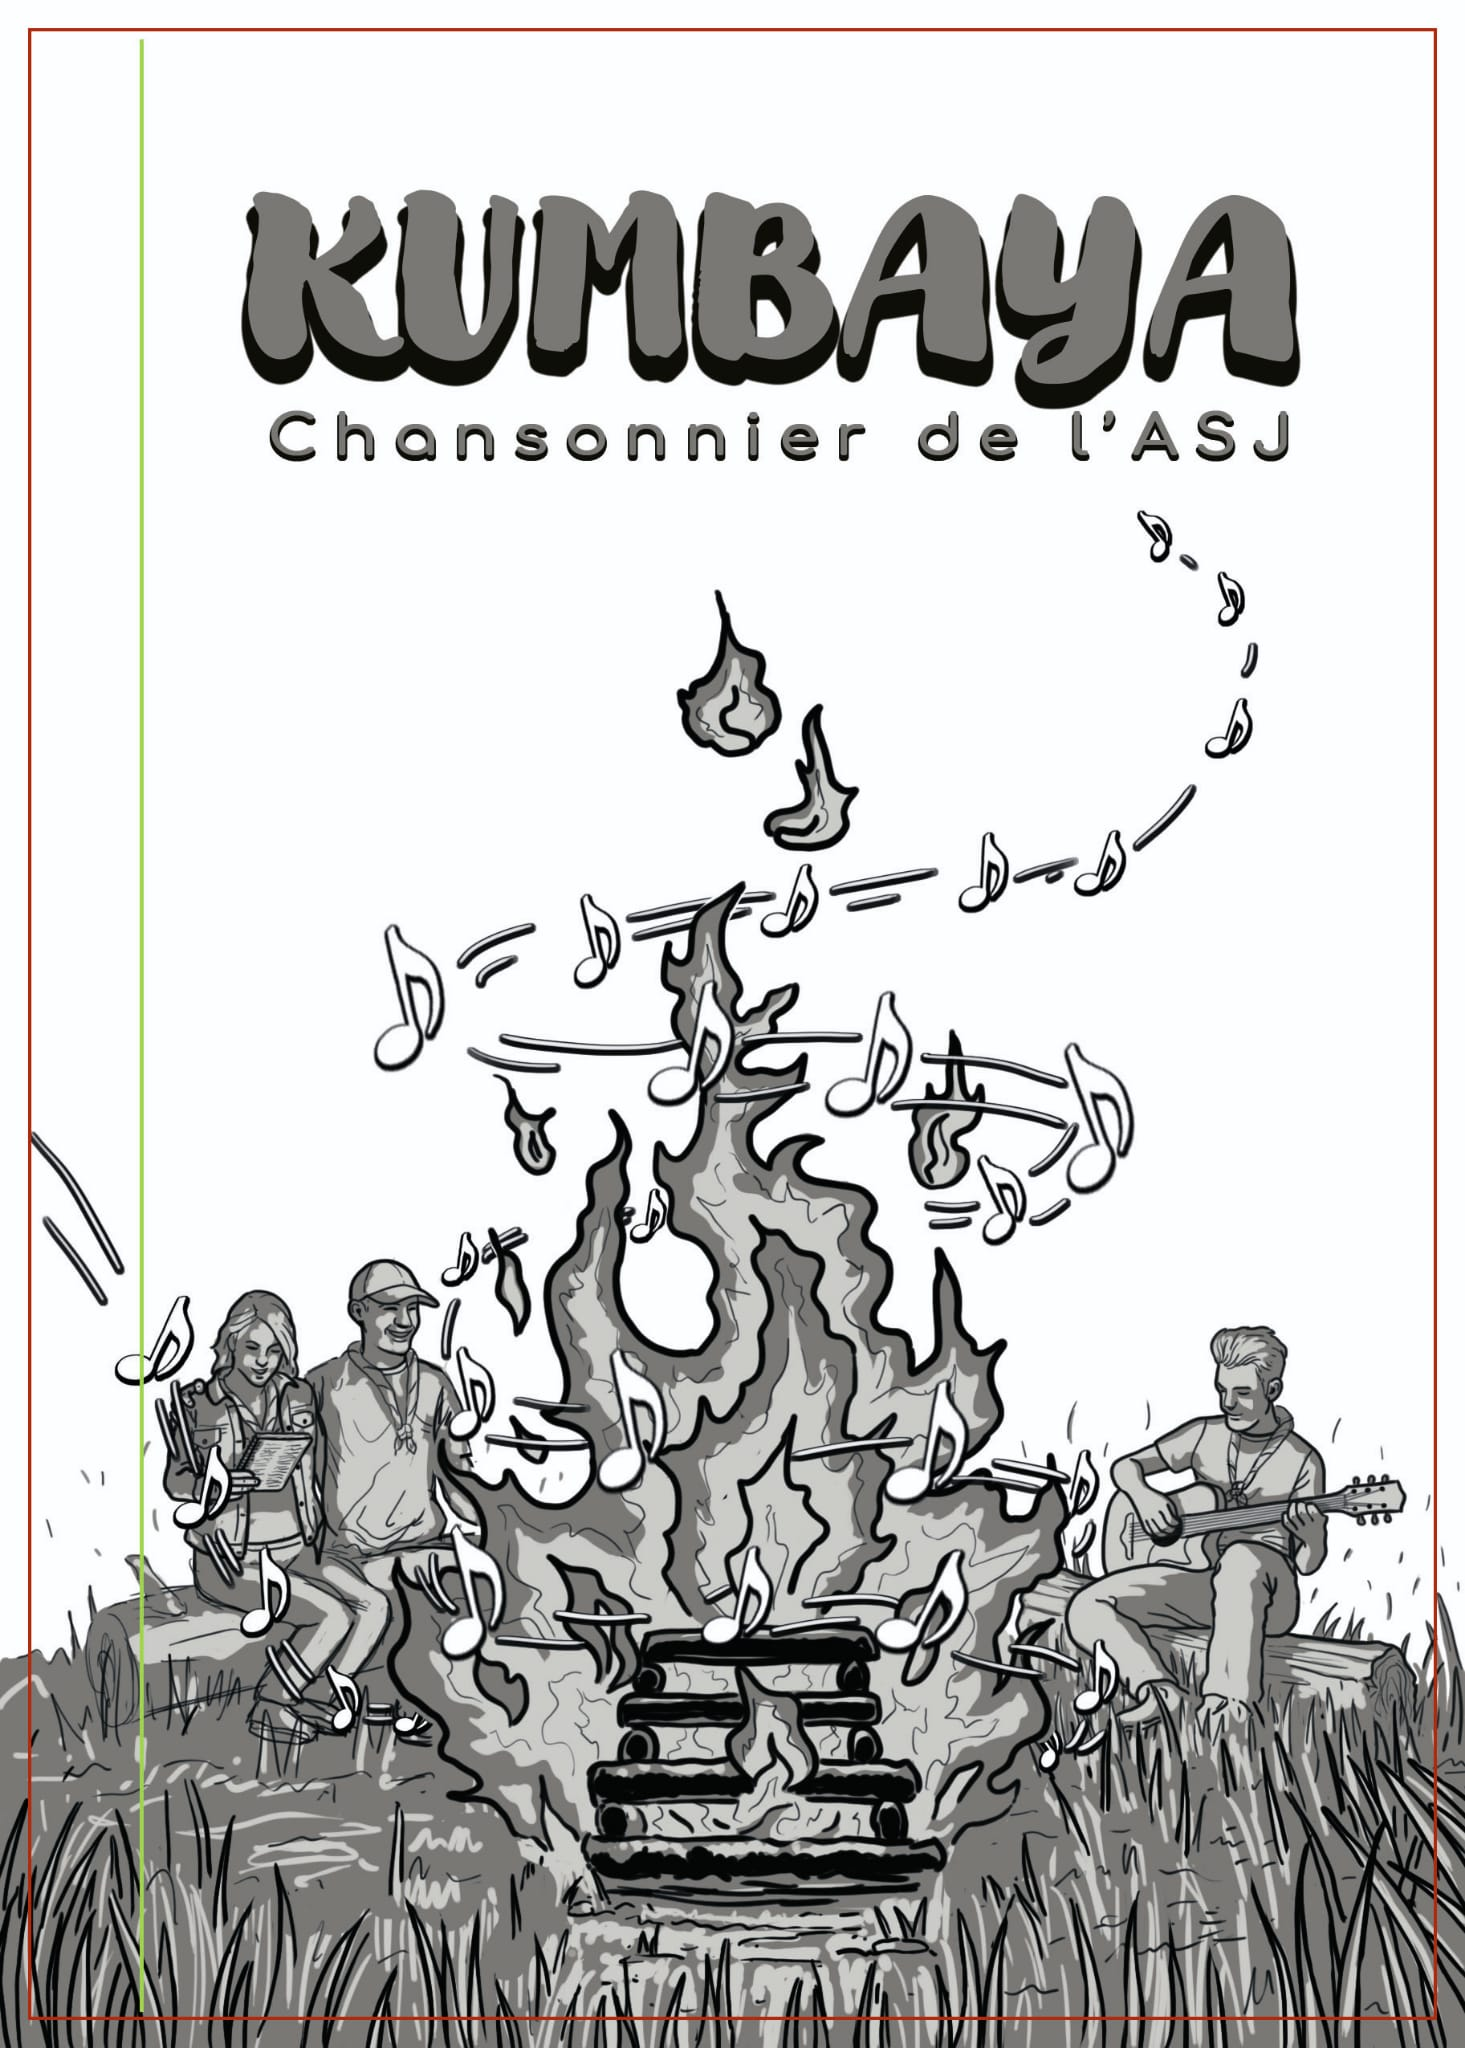
\includegraphics[width=154truemm,height=216truemm]{couverture.jpeg}}}%
}
\newpage
\
\newpage
\clearpage
\restoregeometry

% \showindex[2]{Index alphabétique}{mainindex}
\section*{Avant-propos}
\small Tu tiens entre tes mains la toute nouvelle édition du Kumbaya : le chansonnier de l'Association du Scoutisme Jurassien ! Pensé pour toutes celles et ceux qui aiment pousser la chansonnette autour d'un feu de camp, guitare en bandoulière, ou encore micro à la main pour chanter en mode karaoké grâce à notre playlist Spotify “Kumbaya”. Ce recueil t'accompagnera dans tes moments musicaux et festifs.

Au cœur de sa conception, plusieurs objectifs ont guidé notre équipe. D'abord, nous avons souhaité rafraîchir le répertoire musical, en gardant nos classiques tout en faisant la part belle aux années 1990-2020 et à la découverte de nouvelles et nouveaux artistes. Plusieurs reprises contemporaines sont ainsi mentionnées aux côtés des artistes d'origine.

Ensuite, nous avons souhaité offrir un chansonnier accessible pour encourager la pratique musicale, en particulier à la guitare. Les accords figurent dans ce recueil accompagnés d'une méthodologie pratique pour que les grands rêveurs ainsi que les débutant·e·s osent enfin se lancer à la gratte !
Par ailleurs, notre chansonnier vise à intégrer davantage les branches Louveteaux et Route dans son répertoire. Des chansons pour les plus petit·e·s et autres bans figurent ainsi dans notre table des matières. D'autre part, plusieurs chansons adressées à un public plus majeur dont les paroles portent sur la consommation de substances addictives ainsi que des idées potentiellement violentes, politiques ou morales subjectives de leurs artistes sont marquées du signe *. Notre équipe souhaite laisser à chaque adulte la réflexion du choix des chansons et le soin d'une prévention ou d'une remise en contexte adaptée.

Née d'une idée lancée à l'automne 2022 au large de la mer Égée, cette édition du Kumbaya est le fruit d'un travail collectif, nourri par les propositions des douze groupes de l'ASJ, de longues discussions entre passionné·e·s de chant, et d'un élan enthousiaste printanier pour le faire aboutir à temps pour le camp JUBACA. Son contenu trouve ses origines dans le Kumbaya de l'ASJ (1997), la première édition du Petit Romand (1998), le Faramaz du Groupe Perceval (2013) et la nouvelle édition du P'tit Romand du scoutisme genevois (2023).

Alors que s'élève la première note de la farandole, que crépitent les braises ou que la sono s'allume… nous te souhaitons de belles veillées sous les étoiles!

L'équipe Kumbaya de l'Association du Scoutisme Jurassien (ASJ)

Juillet 2025

\newpage
\begin{multicols}{\nbcols}
	\begin{songs}{}
		\beginsong{1987}[by={Calogero (2017)}]

\beginverse
Tu t'sou\MultiwordChords\[Ré]viens
Les couleurs sur les bas\MultiwordChords\[Sim]kets
Les crayons dans les cas\MultiwordChords\[La]settes
Je rembobine
Tu t'sou\MultiwordChords\[Ré]viens
Tous ces rêves plein nos disq\MultiwordChords\[Sim]uettes
À Paris c'était les S\MultiwordChords\[La]tates
198\MultiwordChords\[Mim]7 \MultiwordChords\[La]
\endverse

\beginchorus
Il \MultiwordChords\[Ré]y a certains jours où \MultiwordChords\MultiwordChords\[La]je reprends mon skate
Et j\MultiwordChords\[Si7]e vais faire un tour en 19\MultiwordChords\[Fa#m]87 \MultiwordChords\[Sol] \MultiwordChords\[Mim] \MultiwordChords\[La]
Il \MultiwordChords\[Ré]y a certains jours dans \MultiwordChords\[La]lesquels je me jette
Et \MultiwordChords\MultiwordChords\[Sim7]je suis de retour en 19\MultiwordChords\[Fa#m]87 \MultiwordChords\[Sol] \MultiwordChords\[Mim] \MultiwordChords\[La]
Tu \MultiwordChords\[Ré]sais de tous ces jours y'a \MultiwordChords\[La]rien que je regrette
Mais \[Sim7]parfois je retourne en \MultiwordChords\[Fa#m]mille neuf cent quatre-vingt-\MultiwordChords\[Sol]sept, en 87
\endchorus

\beginverse
Tu t'souviens
Les survêts et les houppettes
Sabrina et 7 sur 7
Dans la cuisine c'était rien
Que 12 mois sur la planète
L'URSS, INXS
On chantait I want your sex
\endverse

\beginchorus
Refrain
\endchorus

\beginverse
Tu verras bien qu'un jour une chanson dans la tête
Tu l'auras à ton tour ton 1987
Tu verras bien qu'un jour une chanson dans la tête
Tu l'auras à ton tour ton 1987
C'est tout ce que je te souhaite
Tu l'auras à ton tour ton 1987
C'est tout ce que je te souhaite
Tu l'auras à ton tour ton 1987
C'est tout ce que je te souhaite
Tu l'auras à ton tour ton 1987
Tu t'souviens
\endverse
\endsong

\beginsong{99 Luftballons}[by={Nena (1983)}]

\beginverse
\MultiwordChords\[Ré]Hast du etwas \MultiwordChords\[Mim]Zeit für mich ?
Dann \MultiwordChords\[Sol]singe ich ein \MultiwordChords\[La]Lied für dich
Von \MultiwordChords\[Ré]99 \MultiwordChords\[Mim]Luftballons
Auf \MultiwordChords\[Sol]ihrem Weg zum \MultiwordChords\[La]Horizont
\MultiwordChords\[Ré]Denkst du vielleicht \MultiwordChords\[Mim]g'rade an mich
Dann \MultiwordChords\[Sol]singe ich ein \MultiwordChords\[La]Lied für dich
Von \MultiwordChords\[Ré]99 \MultiwordChords\[Mim]Luftballons
Und \MultiwordChords\[Sol]das sowas von \MultiwordChords\[La]sowas kommt
\endverse

\beginverse
99 Luftballons
Auf ihrem Weg zum Horizont
Hielt man für UFOs aus dem All
Darum schickte ein General
Eine Fliegerstaffel hinterher
Alarm zu geben, wenn es so wäre
Dabei waren da am Horizont
Nur 99 Luftballons
\endverse

\beginverse
99 Düsenflieger
Jeder war ein großer Krieger
Hielten sich für Captain Kirk
Das gab ein großes Feuerwerk
Die Nachbarn haben nichts gerafft
Und fühlten sich gleich angemacht
Dabei schoss man am Horizont
Auf 99 Luftballons
\endverse

\beginverse
99 Kriegsminister
Streichholz und Benzinkanister
Hielten sich für schlaue Leute
Witterten schon fette Beute
Riefen Krieg und wollten Macht
Mann, wer hätte das gedacht ?
Dass es einmal soweit kommt
Wegen 99 Luftballons
\endverse

\beginverse
99 Jahre Krieg
Ließen keinen Platz für Sieger
Kriegsminister gibt es nicht mehr
Und auch keine Düsenflieger
Heute ziehe ich meine Runden
Sehe die Welt in Trümmern liegen
Habe einen Luftballon gefunden
Denke an dich und lasse ihn fliegen
\endverse
\endsong

\beginsong{À nos souvenirs}[by={Trois cafés gourmands (2018)},sr={Capo IV}]

\beginverse
Comment puis-je oubl\MultiwordChords\[Lam]ier
Ce coin de para\MultiwordChords\[Fa]dis ?
Ce petit bout de \MultiwordChords\[Do]terre
Où vit encore mon \MultiwordChords\[Sol]père
\endverse

\beginverse
Comment pourrais-je \MultiwordChords\[Lam]faire
Pour me séparer \MultiwordChords\[Fa]d'elle ?
Oublier qu'on est \MultiwordChords\[Do]frères
Belle Corrèze char\MultiwordChords\[Sol]nelle
Oublier ce ma\MultiwordChords\[Lam]tin que tu es Par\MultiwordChords\[Fa]isien
Que t'as de l'eau dans le \MultiwordChords\[Do]vin
Que tu es parti \MultiwordChords\[Sol]loin
\endverse

\beginverse
Ce n'était pas ma faute
On joue des fausses notes
On se trompe de chemin
Et on a du chagrin
On se joue tout un drame
On a des vagues à l'âme
Tu as du mal au cœur
Tu as peur du bonheur
\endverse

\beginverse
Acheter des tableaux
Et des vaches en photo
C'est tout ce que t'as trouvé
Pour te la rappeler
Vous me trouvez un peu con
N'aimez pas ma chanson
\endverse

\beginverse
Vous me croyez bizarre
Un peu patriotard
Le fruit de ma réflexion
Ne touchera personne
Si vos pas ne résonnent
Jamais dans ma région
\endverse

\beginverse
C'est pire qu'une religion
Au-delà d'une confession
Je l'aime à en mourir
Pour le meilleur et pour le pire
Et si je monte au ciel
Il y aura peut-être Joël
\endverse

\beginverse
Guillaume et Jeremy
Et mon cousin Piedri
Yoan sera en voyage
Dans un autre pays
Allez fais tes bagages
Viens rejoindre tes amis
\endverse

\beginverse
On veut du Clody Musette
À en perdre la tête
On veut un dernier Chabrol
Un petit coup de gnôle
Les yeux de nos grands-mères
La voix de nos grands-pères
L'odeur de cette terre
Vue sur les Monédières
\endverse

\beginverse
C'est pire qu'un testament
Au-delà d'une confidence
On est des petits-enfants
De ce joli coin de France
Enterrez-nous vivants
Bâillonnés s'il le faut
Mais prenez soin avant
De remplir notre jabot
\endverse

\beginverse
La relève est pour toi
Notre petit Lucas
On t'laisse en héritage la piste
Nous, on dégage
Le temps nous a gâtés
On en a bien profité
On a des souvenirs en tête
Ce soir, faisons la fête
\endverse

\beginchorus
Acceptez ma rengaine
Elle veut juste dire je t'aime
Soyez sûr, j'en suis fier
J'ai la Corrèze en cathéter
D'être avec vous ce soir
J'ai le cœur qui pétille
Mimi, sers-nous à boire
On a les yeux qui brillent
\endchorus

\beginverse
\bis{Papayapapa, papayapapa, papayapapa
    Paya, papayapapa}{4}
\endverse

\beginchorus
Refrain
\endchorus
\endsong

\beginsong{L'agriculteur}[by={Ridan (2003)}]

\beginverse
J'allume mon p\MultiwordChords\[Lam]oste de tél\MultiwordChords\[Do]é
Pour admir\MultiwordChords\[Sol]er ce qu'il s'y p\MultiwordChords\[Lam]asse
Un milliard\MultiwordChords\[Fa]aire s'envoie en l\MultiwordChords\[Rém]'air
Toute l'at\MultiwordChords\[Mim]mosphère pour voir l'esp\MultiwordChords\[Lam]ace
J'troque son bol d\MultiwordChords\[Lam]'air et sa cuil\MultiwordChords\[Do]lère
Contre un p'tit v\MultiwordChords\[Sol]erre sur ma ter\MultiwordChords\[Lam]rasse
J'en ai ras-le-b\MultiwordChords\[Fa]ol de tout ce bét\MultiwordChords\[Rém]on
J'ai la fol\MultiwordChords\[Mim]ie des grands esp\MultiwordChords\[Lam]aces
\[Lam] \[Do] \[Sol] \[Lam] \brk J'en ai ras-le-b\MultiwordChords\[Fa]ol de tout ce bét\MultiwordChords\[Rém]on
J'ai la fol\MultiwordChords\[Mim]ie des grands esp\MultiwordChords\[Lam]aces
Mais qu'est-ce qui s\MultiwordChords\[Lam]e passe dans nos p'tites t\MultiwordChords\[Do]êtes ?
On s'entasse t\MultiwordChords\[Sol]ous comme des sard\MultiwordChords\[Lam]ines
Dans les grosses b\MultiwordChords\[Fa]oîtes que l'on cons\MultiwordChords\[Rém]erve
Le p'tit pois\MultiwordChords\[Mim]son doit suivre sa l\MultiwordChords\[Lam]igne
\[Lam] \[Do] \[Sol] \[Lam] \brk Dans les grosses b\MultiwordChords\[Fa]oîtes que l'on cons\MultiwordChords\[Rém]erve
Le p'tit pois\MultiwordChords\[Mim]son doit suivre sa l\MultiwordChords\[Lam]igne
\endverse

\beginchorus
Et puis m\MultiwordChords\[Lam]erde! J'ai décid\MultiwordChords\[Do]é de vivre l\MultiwordChords\[Sol]oin sur la col\MultiwordChords\[Lam]line
Vivre s\MultiwordChords\[Fa]eul dans une mais\MultiwordChords\[Rém]on avec la v\MultiwordChords\[Mim]ue sur ma rais\MultiwordChords\[Lam]on
J'préfère vivre p\MultiwordChords\[Lam]auvre avec mon â\MultiwordChords\[Do]me, que vivre r\MultiwordChords\[Sol]iche avec la l\MultiwordChords\[Lam]eur
Et si le b\MultiwordChords\[Fa]lé m'file du bonh\MultiwordChords\[Rém]eur, j'me ferais p\MultiwordChords\[Mim]'têt' agricult\MultiwordChords\[Lam]eur
\MultiwordChords\[Lam] \MultiwordChords\[Do] \MultiwordChords\[Sol] \MultiwordChords\[Lam] \brk Et si le b\MultiwordChords\[Fa]lé m'file du bonh\MultiwordChords\[Rém]eur, j'me ferais p\MultiwordChords\[Mim]'têt' agricult\MultiwordChords\[Lam]eur
\endchorus

\beginverse
Y a trop d'feux rouges dans les grandes villes
J'ai préféré me mettre au vert
J'ai plus d'bonheur à vivre en paix
Que d'm'admirer au fond d'un verre
J'boirai l'eau saine de mon ruisseau
Plutôt qu'l'eau sale du fond de la Seine
Chargée en plomb et en histoire
Que la surface ne laisse plus voir
Chargée en plomb et en histoire
Que la surface ne laisse plus voir
J'ferai des bornes pour m'éloigner
Pour m'retrouver face au miroir
Juste une seconde de vérité
Pour qu'mon passé coule sous les ponts
J'ferai des bornes pour m'éclipser
Pour m'retrouver face à que dalle
Juste une seconde de vérité
Pour contempler ce qu'on est tous
\endverse

\beginchorus
Refrain
\endchorus

\beginverse
Ça fait longtemps que j'n'ai plus vu
Ce coin d'soleil à l'horizon
Ça fait longtemps que j'l'attendais
La petite lueur de la raison
Une petite chanson au clair de lune
Pour réchauffer le cœur de pierre
Le grand retour à l'essentiel
Le feu de bois éclaire le ciel
Le grand retour à l'essentiel
Le feu de bois éclaire le ciel
La mélodie de la nature
Reprend ses droits sur la folie
C'est toute la vie qui nous observe
Que l'on oublie au fil du temps
La mélodie, celle de la vie
Que l'on consume à chaque instant
Tous nos acquis s'écrasent au sol
Et j'ai choisi la clé des champs
Tous nos acquis s'écrasent au sol
Et j'ai choisi la clef des champs
\endverse

\beginchorus
\bis{Refrain}{2}
\endchorus
\endsong

\beginsong{Ah les crocodiles !}[by={Jacques Offenbach (1856), Julien Doré (2024)}]

\beginverse
\MultiwordChords\[Ré]Un crocodile s'en allant à la \MultiwordChords\[La]guerre
\MultiwordChords\[Mi]Disait au revoir \MultiwordChords\[Mi7]à ses petits-\MultiwordChords\[La]enfants
\MultiwordChords\[Ré]Traînant ses pieds, ses pieds dans la pouss\MultiwordChords\[La]ière
\MultiwordChords\[Mi]Il s'en allait combattre les élé\MultiwordChords\[La7]phants
\endverse

\beginchorus
\bis{\MultiwordChords\[Ré]Ah' les crocrocros, les crocrocros, les croco\MultiwordChords\[La7]diles
    Sur les bords du Nil, ils sont partis, n'en parlons \MultiwordChords\[Ré]plus}{2}
\endchorus

\beginverse
Il fredonnait une marche militaire
Dont il mâchait les mots à grosses dents
Quand il ouvrait la gueule tout entière
On croyait voir ses ennemis dedans
\endverse

\beginverse
Il agitait sa grande queue à l'arrière
Comme s'il était d'avance triomphant
Les animaux devant sa mine altière
Dans les forêts s'enfuyaient tout tremblants
\endverse

\beginverse
Un éléphant parut et sur la terre
Se prépara ce combat de géants
Mais près de là courait une rivière
Le crocodile s'y jeta subitement
\endverse

\beginverse
Et tout rempli d'une crainte salutaire
Il s'en retourna vers ses petits-enfants
Notre éléphant, d'une trompe plus fière
Voulut alors accompagner ce chant
\endverse
\endsong

\beginsong{Aïcha}[by={Khaled (1996)},sr={Capo III}]

\beginverse
\MultiwordChords\[Mim] Comme \MultiwordChords\[Do]si je n'ex\MultiwordChords\[Sol]istais \MultiwordChords\[Ré]pas
\MultiwordChords\[Mim] Elle e\MultiwordChords\[Do]st passée à côt\MultiwordChords\[Sol]é de \MultiwordChords\[Ré]moi
\MultiwordChords\[Mim] Sans un \MultiwordChords\[Do]regard, \MultiwordChords\[Sol]reine de \MultiwordChords\[Ré]Saba
\MultiwordChords\[Mim] J'ai \MultiwordChords\[Do]dit “Aïcha, prends, tout \MultiwordChords\[Sol]est pour t\MultiwordChords\[Ré]oi”
\endverse

\beginverse
Voici les perles, les bijoux
Aussi l'or autour de ton cou
Les fruits bien mûrs au goût de miel
Ma vie, Aïcha, si tu m'aimes
J'irai où ton souffle nous mène
Dans les pays d'ivoire et d'ébène
J'effacerai tes larmes, tes peines
Rien n'est trop beau pour une si belle, oh!
\endverse

\beginchorus
\MultiwordChords\[Mim] Aïc\MultiwordChords\[Do]ha, Aïcha, \MultiwordChords\[Sol]écoute-m\MultiwordChords\[Ré]oi
\MultiwordChords\[Mim] Aïc\MultiwordChords\[Do]ha, Aïcha, \MultiwordChords\[Sol]t'en va p\MultiwordChords\[Ré]as
\MultiwordChords\[Mim] Aïc\MultiwordChords\[Do]ha, Aïcha, r\MultiwordChords\[Sol]egarde-m\MultiwordChords\[Ré]oi
\MultiwordChords\[Mim] Aïc\MultiwordChords\[Do]ha, Aïcha, r\MultiwordChords\[Sol]éponds-m\MultiwordChords\[Ré]oi
\endchorus

\beginverse
Je dirai les mots, les poèmes
Je jouerai les musiques du ciel
Je prendrai les rayons du soleil
Pour éclairer tes yeux de reine, oh!
\endverse

\beginchorus
Refrain
\endchorus

\beginverse
\MultiwordChords\[Misus4] \MultiwordChords\[Lam]Elle a dit, Garde tes t\MultiwordChords\[Fa]résors
\MultiwordChords\[Lam]Moi, je vaux mieux que tout ç\MultiwordChords\[Fa]a
\MultiwordChords\[Rém] Des barreaux sont des barreaux, même \MultiwordChords\[Sol]en or
Je veux les \MultiwordChords\[Misus4]mêmes dr\MultiwordChords\[Mi]oits que t\MultiwordChords\[Lam]oi
\MultiwordChords\[Fa] Et du respect pour chaque j\MultiwordChords\[Rém]our
\MultiwordChords\[Rém]Moi, je ne veux que de l'\MultiwordChords\[Misus4]amour \MultiwordChords\[Mi]
\endverse

\beginverse
\MultiwordChords\[Mim] Comme \MultiwordChords\[Do]si je n'ex\MultiwordChords\[Sol]istais \MultiwordChords\[Ré]pas
Elle est passée à côté de moi
Sans un regard, reine de Saba
J'ai dit Aïcha, prends, tout est pour toi
\endverse
\endsong

\beginsong{L'aigle noir}[by={Barbara (1970)}]

\beginverse
\MultiwordChords\[Ré]Un beau jour ou peut-être \MultiwordChords\[La]une nuit
\MultiwordChords\[Mim]Près d'un lac je m'étais endormie
Quand soudain semblant crever le ciel
Et venant de nulle part
Surgit un aigle noir
\endverse

\beginverse
Lentement les ailes déployées
Lentement je le vis tournoyer
Près de moi dans un bruissement d'ailes
Comme tombé du ciel
L'oiseau vint se poser
\endverse

\beginverse
Il avait les yeux couleur rubis
Et les plumes couleur de la nuit
A son front, brillant de mille feux
L'oiseau roi couronné
Portait un diamant bleu
\endverse

\beginverse
De son bec il a touché ma joue
Dans ma main il a glissé son cou
C'est alors que je l'ai reconnu
Surgissant du passé
Il m'était revenu
\endverse

\beginverse
Dis, l'oiseau, oh dis, emmène-moi
Retournons au pays d'autrefois
Comme avant dans mes rêves d'enfant
Pour cueillir en tremblant
Des étoiles, des étoiles
\endverse

\beginverse
Comme avant dans mes rêves d'enfant
Comme avant sur un nuage blanc
Comme avant, allumer le soleil
Etre faiseur de pluie
Et faire des merveilles
\endverse

\beginverse
L'aigle noir dans un bruissement d'ailes
Prit son vol pour regagner le ciel
\endverse

\beginverse
Un beau jour ou peut-être une nuit
Près d'un lac je m'étais endormie
Quand soudain semblant crever le ciel
Et venant de nulle part
Surgit un aigle noir
\endverse
\endsong

\beginsong{Allô le monde}[by={Pauline (2007)},sr={Capo I}]

\beginverse
Il pa\MultiwordChords\[Lam]raît que les nouv\MultiwordChords\[Fa]elles ne \MultiwordChords\[Do]sont pas si b\MultiwordChords\[Sol]onnes
Que le mora\MultiwordChords\[La]l des\MultiwordChords\[Fa]cend
Et que l\MultiwordChords\[Do]es forces t'aband\MultiwordChords\[Sol]onnent
J'en\MultiwordChords\[Lam]tends
Tous les \MultiwordChords\[Fa]gens
Par\MultiwordChords\[Do]ler de tes his\MultiwordChords\[Sol]toires
Que l'ave\MultiwordChords\[Lam]nir qui t'at\MultiwordChords\[Fa]tend
Se joue sur le \MultiwordChords\[Do]fil du ra\MultiwordChords\[Sol]soir
Qu'en est-\MultiwordChords\[Fa]il de l'a\MultiwordChords\[Sol]mour ?
Des \MultiwordChords\[Fa]larmes et de la \MultiwordChords\[Sol]peine ?
De la \MultiwordChords\[Fa]vie de tous les \MultiwordChords\[Sol]jours ?
Et d\MultiwordChords\[Fa]e la paix \MultiwordChords\[Sol]sereine ?
\endverse

\beginchorus
Allô le \MultiwordChords\[Lam]monde \MultiwordChords\[Fa]
\[Lam]Est-ce que tout va b\MultiwordChords\[Sol]ien ?
Allô le mon\MultiwordChords\[Lam]de \MultiwordChords\[Fa]
Je \MultiwordChords\[Lam]n'y comprends plus \MultiwordChords\[Sol]rien
Allô le mon\MultiwordChords\[Lam]de \MultiwordChords\[Fa]
\MultiwordChords\[Lam]Prends soin de \MultiwordChords\[Sol]toi
Allô le mon\MultiwordChords\[Lam]de \MultiwordChords\[Fa]
Ne te laisse \MultiwordChords\[Lam]pas aller \MultiwordChords\[Sol]
Comme \MultiwordChords\[Lam]ç\MultiwordChords\[Fa]a\MultiwordChords\[Lam] \MultiwordChords\[Sol]
\MultiwordChords\[Sol]Comme \MultiwordChords\[Lam]ç\MultiwordChords\[Fa]a\MultiwordChords\[Lam] \MultiwordChords\[Sol]
\endchorus

\beginverse
Quel est le nom du mal dont tu subis la fièvre
Les étranges idéaux, les hystéries funèbres ?
Dis-moi ce que je peux faire de ma petite place
Quels sont les actes et les mots qui peuvent t'aider à faire face ?
Pousser à la révolte
Pour faire le premier pas
Semer pour qu'on récolte
Pour crier mon effroi
\endverse

\beginverse
\[Lam]Allô le \[Rém]monde
\[Fa] Allô le \[Sol]monde
\[Lam]Allô le \[Rém]mond\[Fa]e \[Sol]
Allô le monde
Allô le monde
\endverse

\beginverse
Allô le monde
Est-ce que tout va bien ?
Allô le monde
Allô le monde
Prends soin de toi
Allô le monde
Le monde, le monde, le monde, le monde
Le monde, le monde, le monde, le monde
Allô le monde
Allô le monde, le monde
\endverse
\endsong

\beginsong{L'alphabet scout}[by={Traditionnel}]

\beginverse
Un j\MultiwordChords\[Do]our la troupe campa, A \MultiwordChords\[Sol]A A
La pluie se mit à tomber, \MultiwordChords\[Sol7]B B \MultiwordChords\[Do]B
L'orage a tout cassé, C C \MultiwordChords\[Sol]C
Faillit nous inon\MultiwordChords\[Do]der, A \MultiwordChords\[Sol]B C \MultiwordChords\[Do]D
\endverse

\beginverse
Le chef s'est écrié, E E E
A son adjoint Joseph, F F F
Fais-nous vite à manger, G G G
Les scouts sont sous la bâche E F G H
\endverse

\beginverse
Les pinsons dans leur nid, I l I
Les cerfs dans leur logis, J J J
Chahutent, quel fracas, K K K
Avec les hirondelles, I J K L
\endverse

\beginverse
Joseph nous fit d'la crème, M M M
Et du lapin d'Garenne, N N N
Et même du cacao, O O O
Mes amis quel souper, M N O P
\endverse

\beginverse
Soyez bien convaincus, QQ Q
Que la vie au grand air, R R R
Fortifie la jeunesse, S S S
Et lui rend la santé, Q R S T
\endverse

\beginverse
Maint'nant qu'il ne pleut plus, U U U
Les scouts peuvent se sauver, V V V
Le temps est au beau fixe, X X X
Plus besoin qu'on les aide, U V XZ
\endverse
\endsong

\beginsong{L'amour brille sous les étoiles}[by={Elton John, Tim Rice \- Le Roi Lion (1994)}]

\beginverse
\MultiwordChords\[Sol] C'est terrible c'est aff\MultiwordChords\[Ré]reux \- Quoi ?
Et \MultiwordChords\[Sol]ils se moquent de \MultiwordChords\[Ré]tout \- Qui ?
L'a\MultiwordChords\[Sol]mour s'amène et \MultiwordChords\[Sim]nous pauvres pouilleux
Ils \MultiwordChords\[Mim]nous jettent tous les \MultiwordChords\[La]deux \- Oh !
Sous \MultiwordChords\[Sol]les diamants des \MultiwordChords\[Ré]étoiles
Quel \MultiwordChords\[Sol]magique uni\MultiwordChords\[Ré]vers
Mais\MultiwordChords\[Sol] dans cette ro\MultiwordChords\[Sim]mantique atmosp\MultiwordChords\[Sol]hère
Ça \MultiwordChords\[Fa]sent mauvais dans \MultiwordChords\[Ré]l'air
\endverse

\beginverse
\MultiwordChords\[Sol] L'amour b\MultiwordChords\[Ré]rille sous \MultiwordChords\[Mim]les étoi\MultiwordChords\[Do]les
\MultiwordChords\[Sol] D'une étran\MultiwordChords\[Do]ge lumiè\MultiwordChords\[Ré]re
\MultiwordChords\[Do] La Terre en\MultiwordChords\[Sol]tière
En \MultiwordChords\[Mim]parfaite h\MultiwordChords\[Do]armonie
Vit \MultiwordChords\[Lam]un mo\MultiwordChords\[Fa]ment ro\MultiwordChords\[Ré]yal
\endverse

\beginverse
Je voudrais lui dire je t'aime
Mais comment lui avouer
Mon secret mes problèmes
Impossible
Elle serait trop blessée
\endverse

\beginverse
Quel lourd secret cache-t-il
Derrière tant de rancœur
Moi je sais qu'il est ce roi en exil
Qui règne dans mon coeur
\endverse

\beginverse
L'amour brille sous les étoiles
D'une étrange lumière
La Terre entière
En parfaite harmonie
Vit sa plus belle histoire
\endverse

\beginverse
L'amour brille sous les étoiles
Illuminant leurs coeurs
Sa lumière éclaire à l'infini
Un sublime espoir
\endverse

\beginverse
S'ils s'enfuient vers
Leur rêve ce soir
Dans leur folle ronde
Si notre ami nous dit au revoir
Nous serons seuls au monde
\endverse
\endsong

\beginsong{Amour censure*}[by={Hoshi (2020)}]

\beginverse
\MultiwordChords\[Do] Au pla\MultiwordChords\[Sol]card mes senti\MultiwordChords\[Ré]ments
Surtout ne rien d\MultiwordChords\[Mim]ire, et faire semb\MultiwordChords\[Do]lant
Être à \MultiwordChords\[Sol]part, un peu penc\MultiwordChords\[Ré]hant
Au bout du nav\MultiwordChords\[Mim]ire, je coule doucement
\endverse

\beginverse
\MultiwordChords\[Do] Maman désolée, j'vais pas te mentir
\MultiwordChords\[Sol] C'est dur d'effacer tout ce qui m'attire
\MultiwordChords\[Ré] Un peu dépassée par tous mes dé\MultiwordChords\[Mim]sirs
\MultiwordChords\[Do] Papa c'est vrai, j'ai poussé de travers
\MultiwordChords\[Sol] J'suis une fleur qui se bat entre deux pierres
\MultiwordChords\[Ré] J'ai un cœur niqué par les bonnes maniè\MultiwordChords\[Mim]res
\endverse

\beginchorus
\MultiwordChords\[Do] Est-ce qu'on va un jour en finir
\MultiwordChords\[Sol] Avec la haine et les injures
\MultiwordChords\[Ré] Est-ce que quelqu'un viendra leur dire
\MultiwordChords\[Mim] Qu'on s'aime et que c'est pas impur
\MultiwordChords\[Do] Pour pas que j'pense à en finir
\MultiwordChords\[Sol] Vos coups m'ont donné de l'allure
\MultiwordChords\[Ré] Pour le meilleur et pour le pire
\MultiwordChords\[Mim] J'prendrai sa main un jour c'est sûr
\endchorus

\beginverse
\MultiwordChords\[Sol] Il n'y a pas d'amour cen\MultiwordChords\[Ré]sure
\MultiwordChords\[Mim] Il n'y a que d'l'amour sin\MultiwordChords\[Do]cère
\MultiwordChords\[Sol] Il n'y a pas d'amour cen\MultiwordChords\[Ré]sure
\MultiwordChords\[Mim] Il n'y a que d'l'amour sin\MultiwordChords\[Do]cère
\endverse

\beginverse
Travestir qui je suis vraiment
Faire taire la rumeur
Les mots sont tranchants
Se mentir à s'arracher les dents
Ils cherchent un docteur
On souffre sans être souffrants
\endverse

\beginverse
Maman désolée, j'ai pris tes calmants
C'est pas que j'voulais partir, mais c'est violent
J'voulais juste dormir un peu plus longtemps
Papa t'inquiète j'ai appris à courir
Moi aussi j'veux une famille à nourrir
On s'en fout près de qui j'vais m'endormir
\endverse

\beginchorus
\bis{Refrain}{2}
\endchorus

\beginverse
Il n'y a pas d'amour censure
Il n'y a que d'l'amour sincère
Il n'y a pas d'amour censure
Il n'y a que d'l'amour sincère
\endverse
\endsong

\beginsong{Amsterdam*}[by={Jacques Brel (1964)}]

\beginverse
Dans le p\MultiwordChords\[Lam]ort d'Amsterdam, y a des m\MultiwordChords\[Mim]arins qui chantent
Les rê\MultiwordChords\[Fa]ves qui les hantent, au lar\MultiwordChords\[Mim7]ge d'Amsterdam
Dans le p\MultiwordChords\[Lam]ort d'Amsterdam, y a des ma\MultiwordChords\[Mim]rins qui dorment
Comme d\MultiwordChords\[Fa]es ori\MultiwordChords\[Mi7]flammes le long d\MultiwordChords\[Lam]es berges mornes
Dans le p\MultiwordChords\[Do]ort d'Amsterdam, y a des ma\MultiwordChords\[Sol7]rins qui meurent
Pleins de bi\MultiwordChords\[Lam]ère et de drames aux pre\MultiwordChords\[Mi7]mières lueurs
Mais dans le p\MultiwordChords\[Fa]ort d'Amsterdam, y a des ma\MultiwordChords\[Mim]rins qui naissent
Dans la c\MultiwordChords\[Fa]haleur ép\MultiwordChords\[Mi7]aisse des lang\MultiwordChords\[Lam]ueurs océanes
\endverse

\beginverse
Dans le port d'Amsterdam, y a des marins qui mangent
Sur des nappes trop blanches des poissons ruisselants
Ils vous montrent des dents à croquer la fortune
A décroisser la Lune, à bouffer des haubans
Et ça sent la morue jusque dans le cœur des frites
Que leurs grosses mains invitent à revenir en plus
Puis se lèvent en riant, dans un bruit de tempête
Referment leur braguette et sortent en rotant
\endverse

\beginverse
Dans le port d'Amsterdam, y a des marins qui dansent
En se frottant la panse sur la panse des femmes
Et ils tournent et ils dansent comme des soleils crachés
Dans le son déchiré d'un accordéon rance
Ils se tordent le cou pour mieux s'entendre rire
Jusqu'à ce que tout à coup l'accordéon expire
Alors, le geste grave, alors le regard fier
Ils ramènent leur Batave jusqu'en pleine lumière
\endverse

\beginverse
Dans le port d'Amsterdam, y a des marins qui boivent
Et qui boivent et reboivent, et qui reboivent encore
Ils boivent à la santé des putains d'Amsterdam
De Hambourg ou d'ailleurs, enfin ils boivent aux dames
Qui leur donnent leur joli corps, qui leur donnent leur vertu
Pour une pièce en or, et quand ils ont bien bu
Se plantent le nez au ciel, se mouchent dans les étoiles
Et ils pissent comme je pleure sur les femmes infidèles
Dans le p\MultiwordChords\[Lam]ort d'Amsterdam, dans le p\MultiwordChords\[Mi7]ort d'Amsterdam\MultiwordChords\[Fa-Mi7-Lam]
\endverse
\endsong

\beginsong{Andalouse}[by={Kendji Girac (2014)},sr={Capo I}]

\beginverse
\MultiwordChords\[Mim] Tu viens le s\MultiwordChords\[Sim]oir
\MultiwordChords\[Lam] Danser sur \MultiwordChords\[Sim]des airs de guit\MultiwordChords\[Mim]are
Et puis tu b\MultiwordChords\[Sim]ouges
\MultiwordChords\[Lam] Tes cheveux n\MultiwordChords\[Sim]oirs, tes lèvres r\MultiwordChords\[Mim]ouges
Tu te bal\MultiwordChords\[Sim]ances
\MultiwordChords\[Lam] Le reste n'\MultiwordChords\[Sim]a pas d'import\MultiwordChords\[Mim]ance
Comme un sol\MultiwordChords\[Sim]eil
\MultiwordChords\[Lam] Tu me brûles \MultiwordChords\[Sim]et me réveilles
\MultiwordChords\[Mim]Tu as \MultiwordChords\[Sim]dans les yeux, l\MultiwordChords\[Lam]e Sud et le f\MultiwordChords\[Sim]eu
\MultiwordChords\[Mim]Je t'ai d\MultiwordChords\[Sim]ans la peau
\MultiwordChords\[Lam]Baila, baila, \MultiwordChords\[Sim]oh
\endverse

\beginchorus
\MultiwordChords\[Mim]Toi, toi, \MultiwordChords\[Sim]ma belle Andal\MultiwordChords\[Lam]ouse
Aussi \MultiwordChords\[Sim]belle que jal\MultiwordChords\[Mim]ouse
Quand tu \MultiwordChords\[Sim]danses, le temps s'arr\MultiwordChords\[Lam]ête
Je perds le \MultiwordChords\[Sim]nord, je perds la t\MultiwordChords\[Mim]ête
Toi, \MultiwordChords\[Sim]ma belle Espag\MultiwordChords\[Lam]nole
Quand tu \MultiwordChords\[Sim]bouges tes é\MultiwordChords\[Mim]paules
Je n'vois \MultiwordChords\[Sim]plus le monde aut\MultiwordChords\[Lam]our
C'est peut-\MultiwordChords\[Sim]être ça, l'amour
\endchorus

\beginverse
Des airs d'Orient
Le sourire et le cœur brûlant
Regard ébène
J'aime te voir bouger comme une reine
Ton corps ondule
Déjà mes pensées se bousculent
Comme la lumière
Il n'y a que toi qui m'éclaire
Tu as dans la voix
Le chaud et le froid
Je t'ai dans la peau
Baila, baila, oh
\endverse

\beginchorus
Refrain
\endchorus

\beginverse
Oh-yé-yé-yé, oh-oh, oh-oh
Oh-yé-yé-yé, oh-oh
Oh-yé-yé-yé, oh-oh, oh-oh
Oh-yé-yé-yé, oh-oh
\endverse

\beginchorus
\bis{Refrain}{2}
\endchorus
\endsong

\beginsong{L'arc-en-ciel}[by={Pellisier-Moulin}]

\beginchorus
\MultiwordChords\[Do]Viens mélanger tes cou\MultiwordChords\[Sol]leurs avec \MultiwordChords\[lam]moi
Réveiller le bon\MultiwordChords\[Fa]heur qui \MultiwordChords\[Sol]dort au fond de \MultiwordChords\[Do]toi
Faire jaillir la lu\MultiwordChords\[Sol]mière de nos \MultiwordChords\[Lam]vies
Improviser la \MultiwordChords\[Fa]fête au \MultiwordChords\[Sol]plein cœur de la \MultiwordChords\[Do]nuit
\endchorus

\beginverse
\MultiwordChords\[Fa]Tu connais la mi\MultiwordChords\[Sol]sère \MultiwordChords\[Do]qui condamne au si\MultiwordChords\[Lam]lence :
\MultiwordChords\[Fa]Prends la main de tes \MultiwordChords\[Sol]frères, i\MultiwordChords\[Do]nvente un pas \MultiwordChords\[Fa]dans\MultiwordChords\[Sol]e !
\endverse

\beginverse
Tu refoules tes larmes dans ta gorge nouée :
Oublie le bruit des armes, réapprends à chanter !
\endverse

\beginverse
Tu t'opposeras à la force qui tue la liberté :
Entrouvre ton écorce au soleil de l'été !
\endverse

\beginverse
Tu rêves d'innocence au lieu d'hypocrisie :
Retrouve ton enfance, recommence ta vie !
\endverse

\beginverse
Tu pardonnes sa haine au frère qui t'a blessé :
Laisse tomber ta gêne, donne-lui un baiser !
\endverse
\endsong

\beginsong{Aux arbres citoyens}[by={Yannick Noah (2006)},sr={Capo I}]

\beginverse
Le \MultiwordChords\[Mim]ciment dans les plaines coule jusqu'aux montagnes
Poi\MultiwordChords\[Ré]son dans les fontaines, dans nos \MultiwordChords\[Do]campagnes
De c\MultiwordChords\[Mim]yclones en rafales, notre histoire prend l'eau
Res\MultiwordChords\[Ré]te notre idéal, fa\MultiwordChords\[Do]ire les beaux
\endverse

\beginverse
S'acheter de l'air en barre, remplir la balance
Quelques pétrodollars, contre l'existence
De l'Équateur aux pôles, ce poids sur nos épaules
De squatteurs éphémères, maintenant, c'est plus drôle
\endverse
\beginchorus
\MultiwordChords\[Mim]Puisqu'il faut changer les choses
A\MultiwordChords\[Ré]ux arbres cito\MultiwordChords\[Do]yens
\MultiwordChords\[Mim]Il est grand temps qu'on propose
\MultiwordChords\[Ré]Un monde \MultiwordChords\[Do]pour demain
\endchorus

\beginverse
Aux arbres citoyens, quelques baffes à prendre
La veille est pour demain, des baffes à rendre
Faire tenir debout une armée de roseaux
Plus personne à genoux, fais passer le mot
\endverse

\beginverse
C'est vrai la Terre est ronde, mais qui viendra nous dire
Qu'elle l'est pour tout le monde et les autres à venir
\endverse

\beginverse
\bis{Refrain}{2}
\endverse
\beginverse
\MultiwordChords\[Ré] Plus le temps de savoir à qui \MultiwordChords\[Mim]la faute
\MultiwordChords\[Ré] De compter sur la chance ou \MultiwordChords\[Do]les autres
\MultiwordChords\[Lam7] Maintenant, on se \MultiwordChords\[Mim]bat
A\MultiwordChords\[Do]vec toi, moi, j'y croi\MultiwordChords\[Mim]s
\endverse

\beginchorus
Refrain
\endchorus
\endsong

\beginsong{L'aventurier}[by={Indochine (1982)}]

\beginverse
\MultiwordChords\[Mim]Égaré dans la \MultiwordChords\[Do]vallée infernale
Le \MultiwordChords\[Sol]héros s'appelle \MultiwordChords\[Lam]Bob Morane
\MultiwordChords\[Mim]À la recherche de l'\MultiwordChords\[Do]Ombre Jaune
Le \MultiwordChords\[Sol]bandit s'appelle Mister \MultiwordChords\[Lam]Kali Jones
\MultiwordChords\[Mim]Avec l'ami Bill \MultiwordChords\[Do]Ballantine
\MultiwordChords\[Sol]Sauvé de justesse des \MultiwordChords\[Lam]crocodiles
\MultiwordChords\[Mim]Stop au trafic des \MultiwordChords\[Do]Caraïbes
\MultiwordChords\[Sol]Escale dans l'opération \MultiwordChords\[Lam]Nadawieb
\endverse

\beginverse
\bis{\MultiwordChords\[Mim]La lalalaaa la l\MultiwordChords\[Do]alalaa, \MultiwordChords\[Sol]La lalala la \MultiwordChords\[Lam]lala-lalaa}{2}
\endverse

\beginverse
Le cœur tendre dans le lit de Miss Clark
Prisonnière du Sultan de Jarawak
En pleine terreur à Manicouagan
Isolé dans la jungle birmane
Emprisonnant les flibustiers
L'ennemi est démasqué
On a volé le collier de Civa
Le Maharadjah en répondra
\endverse

\beginverse
\bis{La lalalaaa la lalalaa, La lalala la lala-lalaa}{2}
\endverse
\beginchorus
\MultiwordChords\[Lam]Et soudain surgit \MultiwordChords\[Mim]face au vent
Le \MultiwordChords\[Sol]vrai héros de \MultiwordChords\[Ré]tous les temps
\MultiwordChords\[Lam]Bob Morane contre \MultiwordChords\[Mim]tout chacal
L'a\MultiwordChords\[Sol]venturier contre \MultiwordChords\[Ré]tout guerrier
\MultiwordChords\[Lam]Bob Morane contre \MultiwordChords\[Mim]tout chacal
L'a\MultiwordChords\[Sol]venturier contre \MultiwordChords\[Ré]tout guerrier
\endchorus

\beginverse
Dérivant à bord du Sampang
L'aventure au parfum d'Ylalang
Son surnom, Samouraï du Soleil
En démantelant le gang de l'Archipel
L'otage des guerriers du Doc Xhatan
Il s'en sortira toujours à temps
Tel l'aventurier solitaire
Bob Morane est le roi de la Terre
\endverse

\beginverse
\bis{La lalalaaa la lalalaa, La lalala la lala-lalaa}{2}
\endverse

\beginchorus
Refrain
\endchorus
\endsong

\beginsong{Balade jurassienne*}[by={Christophe Meyer (2003)}]

\beginverse
\MultiwordChords\[Do] Il pleut \MultiwordChords\[Fa]toujours à Pleu\MultiwordChords\[Do]jouse
Quand le temps s\MultiwordChords\[Sol]'éclaire à Réc\MultiwordChords\[Do]lère
J'ai cou\MultiwordChords\[Fa]ru à Courro\MultiwordChords\[Do]ux
M'émerveil\MultiwordChords\[Sol]ler à Merv\MultiwordChords\[Do]elier
\MultiwordChords\[Fa] Si j'ai failli manquer F\MultiwordChords\[Do]ahy
\MultiwordChords\[Fa] Je ne vais pas rater Les Ge\MultiwordChords\[Do]nevez
\MultiwordChords\[Lam] J'fais aussi un saut à Saul\MultiwordChords\[Sol]cy
Pour cette balade jura\MultiwordChords\[Do]ssienne
\endverse

\beginverse
\MultiwordChords\[Rém]La \MultiwordChords\[Sol]la \MultiwordChords\[Do]la la la \MultiwordChords\[Fa]la
\MultiwordChords\[Rém]la la la \MultiwordChords\[Sol]la la la \MultiwordChords\[Do]la
\endverse

\beginverse
J'ai visité mes amies d'Alle
Vic à Vicques puis celle de Lucelle
Assez près d'elle à Séprais
Elle m'a dit vers ma ferme à Vermes
Qu'elle était soûle à Soulce
Elle voulait que je la plaigne à Pleigne
Les cheveux dans l'vent à Damvant
C'est une balade jurassienne
\endverse

\beginverse
Chatouilleux à Châtillon
J'ai lu le Coran à Corban
Perdu mon savon à Courchavon
C'était dans une rose maison – j'ai vu
Le bon et la folle de Bonfol
Les soldats s'aligner à Lugnez
Se faire couper les courtes mèches
Dans cette balade jurassienne
\endverse

\beginverse
Quand vous montiez à Montignez
J'ai embrassé la joue du r'gard
À Charmoille sur un char de paille
Mis ma ceinture à St-Ursanne
Je recours à Rocourt
Car c'est aux Bois qu'on boit
Le taux d'alcool à Montenol
Dans cette balade jurassienne
\endverse

\beginverse
J'avais l'air affreux à Damphreux
Au court de la beuverie d'Ocourt
Même pas eu l'temps d'cuver à Coeuve
Pour s'bourrer l'gnon à Bourrignon
Quand les copains burent à Bure
Beurré au Raisin d'Beurnevésin
C'était soit hier à Soyhières ou peut-être avant-hier
dans cette balade jurassienne, je sais plus
\endverse

\beginverse
Un peu maraud à Muriaux
J'ai volé des pommes aux Pommerats
Mangé mon melon à Montmelon
Qu'avait un goût moite à Goumois
J'ai soupé à Soubey
Sans faire de bruit à Buix
J'm'endors sur la roche de Roche-d'Or
Pour cette balade jurassienne
\endverse
\endsong

\beginsong{La ballade des gens heureux}[by={Gérard Lenorman (1975)},sr={Capo V}]

\beginverse
Notre \MultiwordChords\[Do]vieille Terre est une étoile
Où toi aussi tu \MultiwordChords\[Rém]brilles un \MultiwordChords\[Sol]peu
\bis{Je viens te \MultiwordChords\[Rém]chanter \MultiwordChords\[Sol7]la bal\MultiwordChords\[Do]lade
    La ball\MultiwordChords\[Rém]ade des \MultiwordChords\[Sol7]gens heu\MultiwordChords\[Do]reux}{2}
\endverse

\beginverse
Tu n'as pas de titre ni de grade
Mais tu dis tu quand tu parles à Dieu
\bis{Je viens te chanter la ballade
    La ballade des gens heureux}{2}
\endverse

\beginverse
Journaliste pour ta première page
Tu peux écrire tout ce que tu veux
\bis{Je t'offre un titre formidable
    La ballade des gens heureux}{2}
\endverse

\beginverse
Toi qui a planté cet arbre
Dans ton petit jardin de banlieue
\bis{Je viens te chanter la ballade
    La ballade des gens heureux}{2}
\endverse

\beginverse
Il s'endort et tu le regardes
Comme un enfant, il te ressemble un peu
\bis{On vient lui chanter la ballade
    La ballade des gens heureux}{2}
\endverse

\beginverse
Toi la star du haut de ta vague
Descends vers nous tu nous verras mieux
\bis{On vient te chanter la ballade
    La ballade des gens heureux}{2}
\endverse

\beginverse
Roi de la drague et de la rigolade
Rouleur, flambeur ou gentil petit vieux
\bis{On vient te chanter la ballade
    La ballade des gens heureux}{2}
\endverse

\beginverse
Comme un choeur dans une cathédrale
Comme un oiseau qui fait ce qu'il veut
\bis{On vient te chanter la ballade
    La ballade des gens heureux}{2}
\endverse
\endsong

\beginsong{La ballade nord-irlandaise*}[by={Renaud (1991)}]

\beginverse
J'ai voulu plant\MultiwordChords\[Sol]er un \MultiwordChords\[Do]orang\MultiwordChords\[Sol]er
Là où la chan\MultiwordChords\[Mim]son n'en \MultiwordChords\[Lam]verra ja\MultiwordChords\[Ré]mais
Là où les \MultiwordChords\[Sol] arbres n'ont jamais don\MultiwordChords\[Mim]né
Que \MultiwordChords\[Do]des gre\MultiwordChords\[Sol]nades \MultiwordChords\[Do]dégoupil\MultiwordChords\[Sol]lées
\endverse

\beginverse
Jusqu'à Derry ma bien aimée
Sur mon bateau j'ai navigué
J'ai dit aux hommes qui se battaient
Je viens planter un oranger
\endverse

\beginverse
Buvons un verre, allons pêcher
Pas une guerre ne pourra durer
Lorsque la bière et l'amitié
Et la musique nous feront chanter
\endverse

\beginverse
Tuez vos dieux à tout jamais
Sous aucune croix l'amour ne se plaît
Ce sont les hommes, pas les curés
Qui font pousser les orangers
\endverse

\beginverse
Je voulais planter un oranger
Là où la chanson n'en verra jamais
Il a fleuri et il a donné
Les fruits sucrés de la liberté
\endverse
\endsong

\beginsong{La batelière}[by={Traditionnel}]

\beginverse
\MultiwordChords\[Do] Gentille batelière, \MultiwordChords\[Sol]laisse-là \MultiwordChords\[Sol7]ton ba\MultiwordChords\[Do]teau
Préfère à ta chaumière \MultiwordChords\[Sol]les honneurs \MultiwordChords\[Sol7]du châ\MultiwordChords\[Do]teau
\MultiwordChords\[Sol]J'irai cueil\MultiwordChords\[Sol7]lir \MultiwordChords\[Do]la fleur nouvelle
\MultiwordChords\[Ré]Chaque matin pour \MultiwordChords\[Sol]toi
Tu choisi\MultiwordChords\[Sol7]ras \MultiwordChords\[Do]rubis, dentelles
\MultiwordChords\[Ré]Blanche viens avec \MultiwordChords\[Sol]moi !
\endverse

\beginchorus
\MultiwordChords\[Sol] Non, non, non, non J'a\MultiwordChords\[Do]ime mieux mon p'tit bateau
Ma \MultiwordChords\[Sol]rame fle\MultiwordChords\[Sol7]xible sur l'\MultiwordChords\[Do]onde paisible
Et ma chaumière au bord de l'eau
Tra \MultiwordChords\[Sol]la la la \MultiwordChords\[Sol7]la la la \MultiwordChords\[Do]la la la la
La \MultiwordChords\[Sol]la la la \MultiwordChords\[Sol7]la, la \MultiwordChords\[Do]la la la la, la \MultiwordChords\[Fa]la la la \MultiwordChords\[Sol]la la \MultiwordChords\[Do]la la la la
La \MultiwordChords\[Sol]la la la \MultiwordChords\[Sol7]la, la \MultiwordChords\[Do]la la la la, la \MultiwordChords\[Fa]la la la \MultiwordChords\[Sol]la la \MultiwordChords\[Do]la
\endchorus

\beginverse
Belle enfant qu'au rivage on entend chaque soir
Malgré les vents, l'orage, dire des chants d'espoir !
Tu reverras dans la vallée
Tes chalets et tes bois
Tu ne seras plus isolée
Blanche viens avec moi !
\endverse

\beginverse
Rien ne trouble ton âme, rien ne trouble ton cœur
Tu doutes de ma flamme, tu ris de ma douleur
Que te faut-il enfant cruelle Pour vaincre ton dédain
Te faire oublier ta nacelle ?
Veux-tu mon cœur, ma main ?
\endverse

\beginverse
Ah ! Ah ! Cette fois, mon seigneur
Tra la la la
Je veux bien vous donner mon cœur
Tra la la la
\endverse
\endsong

\beginsong{Le beau tambour}[by={Henri Dès (1986)}]

\beginverse
\bis{J'ai re\MultiwordChords\[Mi]çu, plan, plan
    J'ai reçu, plan, plan
    J'ai reçu un b\MultiwordChords\[Si7]eau tamb\MultiwordChords\[Mi]our
    Et je joue, plan, plan
    Et je joue, plan, plan
    Et je joue quand \MultiwordChords\[Si7]il fait j\MultiwordChords\[Mi]our
    Et quand \MultiwordChords\[La]il fait n\MultiwordChords\[Mi]uit, et le m\MultiwordChords\[La]ercre\MultiwordChords\[Mi]di
    Et quand p\MultiwordChords\[La]apa d\MultiwordChords\[Mi]ort enc\MultiwordChords\[Si7]ore
    Et pour l\MultiwordChords\[Mi]es vois\MultiwordChords\[Si7]ins, le dima\MultiwordChords\[Mi]nche mat\MultiwordChords\[Si7]in
    Je vais d\MultiwordChords\[Mi]ans le co\MultiwordChords\[Si7]rrid\MultiwordChords\[Mi]or
}{6}
\endverse
\endsong

\beginsong{Bella ciao*}[by={Auteur anonyme (1944)},sr={Capo V}]

\beginverse
Una mat\MultiwordChords\[Lam]tina mi son sveg\MultiwordChords\[Lam]liato
O bella \MultiwordChords\[Lam]ciao, bella ciao, bella \MultiwordChords\[Mi7]ciao ciao ciao
Una mat\MultiwordChords\[Rém]tina mi son sveg\MultiwordChords\[Lam]liato
Eo ho tro\MultiwordChords\[Mi7]vato l'inva\MultiwordChords\[Lam]sor
\endverse

\beginverse
O partigiano portami via
O bella ciao, bella ciao, bella ciao ciao ciao
O partigiano portami via
Che mi sento di morir
\endverse

\beginverse
E se io muoio da partigiano
O bella ciao, bella ciao, bella ciao ciao ciao
E se io muoio da partigiano
Tu mi devi seppellir
\endverse

\beginverse
Mi seppellire lassù in montagna
O bella ciao, bella ciao, bella ciao ciao ciao
Mi seppellire lassù in montagna
Sotto l'ombra di un bel fiore
\endverse

\beginverse
E le gente che passeranno
O bella ciao, bella ciao, bella ciao ciao ciao
E le genti che passeranno
Mi diranno: Che bel fior
\endverse

\beginverse
È questo il fiore del partigiano
O bella ciao, bella ciao, bella ciao ciao ciao
È questo il fiore del partigiano
Morto per la libertà
\endverse
\endsong

\beginsong{Berceuse tchèque}[by={Traditionnel}]

\beginverse
\MultiwordChords\[Do]Ecoute la prière
Qui du camp monte vers T\MultiwordChords\[Sol7]oi
\bis{Vers la grande lumiè\MultiwordChords\[Do]re
    \MultiwordChords\[Rém]Vers la pa\MultiwordChords\[Sol7]ix et vers la j\MultiwordChords\[Do]oie
}{2}
\endverse

\beginverse
Illumine la route
Où le monde nous attend
\bis{Que suivant la loi scoute
    Nous aidions les pauvres gens}{2}
\endverse

\beginverse
Donne à notre patrie
Divisée en ses frontières
\bis{La paix qui fut promise
    A ceux qui s'aiment en frères}{2}
\endverse
\endsong

\beginsong{Les bêtises}[by={Henri Dès (1991)}]

\beginchorus
\MultiwordChords\[Mi] Zoum zoum zoum-zoum-zoum
Zoum zouzoum \MultiwordChords\[Si7]zoum-\MultiwordChords\[Mi]zoum
\MultiwordChords\[Mi] C'est à l'école, tagadaga\MultiwordChords\[Si7]da
\MultiwordChords\[Mi] Qu'on apprend les bêti\MultiwordChords\[Si7]ses
\MultiwordChords\[Mi] C'est à l'école, tagadaga\MultiwordChords\[Si7]da
\MultiwordChords\[Mi] Qu'on apprend les bêti\MultiwordChords\[Si7]ses
\endchorus

\beginverse
Le grand Dédé — poil poil au nez
Devant toute la c\MultiwordChords\[Mi]lasse
\MultiwordChords\[Si7]Monte au tableau — poil poil au dos
Pour faire des gri\MultiwordChords\[Mi]maces
\endverse

\beginchorus
Refrain
\endchorus

\beginverse
Quand le Julien — poil poil aux mains
Raconte ses histoires
Elles sont si bêtes — poil aux chaussettes
Qu'on pleure dans nos mouchoirs
\endverse

\beginchorus
Refrain
\endchorus

\beginverse
Et la maîtresse — poil poil aux tresses
Qui pousse des soupirs
Quand Marion — poil au menton
Attrape le fou rire
\endverse

\beginchorus
Refrain
\endchorus

\beginverse
Et puis y'a moi — poil poil au doigt
Qui marche à quatre pattes
Pour chatouiller — poil au mollet
Ma voisine de droite
\endverse

\beginchorus
Refrain
\endchorus

\beginverse
Y'a la Thérèse — poil à la chaise
C'est la plus rigolote
Quand elle s'asseye — poil aux orteils
On lui voit sa culotte
\endverse

\beginchorus
Refrain
\endchorus

\beginverse
Heureusement — poil poil aux dents
Quand vient la sonnerie
Tout le monde s'arrête — poil aux baskets
Par ici la sortie
\endverse

\beginchorus
Refrain
\endchorus

\beginverse
Zoum zoum zoum-zoum-zoum
Zoum zouzoum zoum-zoum
\endverse
\endsong

\beginsong{Le bleu lumière}[by={Cerise Calixte \- Vaïana (2016)},sr={Capo IV}]

\beginverse
Le b\MultiwordChords\[Do]leu du ciel n'est pas le bleu de la m\MultiwordChords\[Rém]er
Ce bleu que moi je pr\MultiwordChords\[Lam]éfère
Sans vraiment savoir po\MultiwordChords\[Fa]urquoi
\MultiwordChords\[Do]J'aimerais tant rester fidèle à m\MultiwordChords\[Rém]a terre
Oublier le vent éph\MultiwordChords\[Lam]émère
J'ai essayé tant de f\MultiwordChords\[Fa]ois
J'ai beau d\MultiwordChords\[Lam]ire je reste, je ne partirai pas
Chacun d\MultiwordChords\[Sol]e mes gestes, chacun de mes pas
Me ram\MultiwordChords\[Do]ènent sans cesse
Malgré les promesses
Vers c\MultiwordChords\[Fam]e bleu lumière
L'hori\MultiwordChords\[Do]zon où la mer touche le ciel
Et \MultiwordChords\[Sol]m'appelle
Cache un trés\MultiwordChords\[Lam]or
Que tous ig\MultiwordChords\[Fa]norent
C'est le v\MultiwordChords\[Do]ent, doucement qui se lève
Et me r\MultiwordChords\[Sol]évèle
Le bleu de l'\MultiwordChords\[Lam]eau
Si je p\MultiwordChords\[Fam]ars j'irai plus loin et toujours plus haut
\endverse

\beginverse
Il faut aimer mon île et son histoire
Pour ceux qui veulent encore y croire
Oublier le temps qui passe
Il faut aimer mon île et son histoire
Et garder encore l'espoir
Un jour je trouverai ma place
Je peux les guider
Les rendre plus grands
Les accompagner
Je prendrai le temps
Mais cette voie cachée
Pense tout autrement
Je ne comprends pas
Le soleil vient danser sur la mer éternelle
Mais tous ignorent
Ces reflets d'or
Elle m'attend sous un tapis de lumière
La mer m'appelle
Moi je veux voir
Derrière les nuages de nouveaux rivages
L'horizon où la mer touche le ciel
Et m'appelle
Cache un trésor
Que tous ignorent
C'est le vent doucement qui se lève
Et me révèle
J'ai le droit
D'aller là-bas
\endverse
\endsong

\beginsong{Blowin' in the wind}[by={Bob Dylan (1962)}]

\beginverse
\MultiwordChords\[Ré]How many \MultiwordChords\[Sol]roads must a \MultiwordChords\[La]man walk \MultiwordChords\[Ré]down
Before you \MultiwordChords\[Sol]call him a \MultiwordChords\[Ré]man ?
\MultiwordChords\[Ré]How many \MultiwordChords\[Sol]seas must a \MultiwordChords\[La]white dove \MultiwordChords\[Ré]sail
Before she \MultiwordChords\[Sol]sleeps in the \MultiwordChords\[La]sand ?
Yes, and \MultiwordChords\[Ré]how many \MultiwordChords\[Sol]times must the \MultiwordChords\[La]cannonballs \MultiwordChords\[Ré]fly
Before they're \MultiwordChords\[Sol]forever \MultiwordChords\[Ré]banned ?
\endverse

\beginchorus
\MultiwordChords\[Sol]The answer, \MultiwordChords\[La]my friend, \MultiwordChords\[Ré]is blowin' in the \MultiwordChords\[Sol]wind
The answer is \MultiwordChords\[La]blowin' in the \MultiwordChords\[Ré]wind
\endchorus

\beginverse
Yes, and how many years must a mountain exist
Before it is washed to the sea ?
Yes, and how many years can some people exist
Before they're allowed to be free ?
Yes, and how many times can a man turn his head
And pretend that he just doesn't see ?
\endverse

\beginchorus
Refrain
\endchorus

\beginverse
Yes, and how many times must a man look up
Before he can see the sky ?
Yes, and how many ears must one man have
Before he can hear people cry ?
Yes, and how many deaths will it take 'til he knows
That too many people have died ?
\endverse

\beginchorus
Refrain
\endchorus
\endsong

\beginsong{Le blues du businessman}[by={Claude Dubois, Starmania (1978)}]

\beginverse
\MultiwordChords\[Mim]J'ai du succ\MultiwordChords\[La]ès dans mes affa\MultiwordChords\[Ré]ires
J'ai du succ\MultiwordChords\[Sol]ès dans mes am\MultiwordChords\[Do]ours
Je change souvent de secrét\MultiwordChords\[Si7]aire
\MultiwordChords\[Mim]J'ai mon bur\MultiwordChords\[La]eau en haut d'une t\MultiwordChords\[Ré]our
D'où je vois \MultiwordChords\[Sol]la ville à l'en\MultiwordChords\[Do]vers
D'où je contrôle mon uni\MultiwordChords\[Si7]vers
\endverse

\beginverse
J'passe la moitié de ma vie en l'air
Entre New York et Singapour
Je voyage toujours en première
J'ai ma résidence secondaire
Dans tous les Hilton de la Terre
J'peux pas supporter la misère
\endverse

\beginverse
Au moins es-tu heureux
J'suis pas heureux mais j'en ai l'air
J'ai perdu le sens de l'humour
Depuis qu'j'ai le sens des affaires
J'ai réussi et j'en suis fier
Au fond je n'ai qu'un seul regret
J'fais pas ce que j'aurais voulu faire
\endverse

\beginverse
\MultiwordChords\[La] J'aurais voulu être un ar\MultiwordChords\[Ré]tiste
\MultiwordChords\[Sol] Pour pouvoir faire mon numér\MultiwordChords\[Fa#7]o
Quand l'avion se pose sur la \MultiwordChords\[Mim]piste
\MultiwordChords\[La] À Rotterdam ou à \MultiwordChords\[Ré]Rio

\MultiwordChords\[La] J'aurais voulu être un chan\MultiwordChords\[Ré]teur
\MultiwordChords\[Sol] Pour pouvoir crier qui je s\MultiwordChords\[Fa#7]uis
J'aurais voulu être un au\MultiwordChords\[Mim]teur
\MultiwordChords\[La] Pour pouvoir inventer ma \MultiwordChords\[Ré]vie
Pour pouvoir inventer ma v\MultiwordChords\[Fa#7]i\MultiwordChords\[La]e
\endverse

\beginverse
J'aurais voulu être un acteur
Pour tous les jours changer de peau
Et pour pouvoir me trouver beau
Sur un grand écran en couleur
Sur un grand écran en couleur
\endverse

\beginverse
J'aurais voulu être un artiste
Pour avoir le monde à refaire
Pour pouvoir être un anarchiste
Et vivre comme un millionnaire
Et vivre comme un millionnaire
\endverse

\beginverse
J'aurais voulu être un artiste
Pour faire du laid, pour faire du beau
Pour pouvoir dire pourquoi j'existe
Oui, oui, oui
Merci beaucoup
\endverse
\endsong

\beginsong{La Bohème}[by={Charles Aznavour (1966)},sr={Capo III}]

\beginverse
\MultiwordChords\[Rém]Je vous parle d'un temps
Que les moins de vingt ans
Ne peuvent pas con\MultiwordChords\[Lam]naître
Montmartre en ce temps-\MultiwordChords\[Rém]là
Accrochait ses li\MultiwordChords\[Lam]las
Jusque sous nos fenêtres
Et si l'humble \MultiwordChords\[Rém]garni
Qui nous servait de nid
Ne payait pas de mi\MultiwordChords\[Lam]ne
C'est là qu'on s'est \MultiwordChords\[Rém]connu
Moi qui criait \MultiwordChords\[Mi7]famine
Et toi qui posais n\MultiwordChords\[Lam]ue
\endverse

\beginchorus
La Bo\MultiwordChords\[Rém]hème, la Bo\MultiwordChords\[Lam]hème
Ça voulait \MultiwordChords\[Rém]dire
On \MultiwordChords\[Mi7]est heu\MultiwordChords\[Lam]reux
La Bo\MultiwordChords\[Rém]hème, la Bo\MultiwordChords\[Lam]hème
Nous ne man\MultiwordChords\[Rém]gions qu'un \MultiwordChords\[Mi7]jour sur \MultiwordChords\[Lam]deux
\endchorus

\beginverse
Dans les cafés voisins
Nous étions quelques-uns
Qui attendions la gloire
Et bien que miséreux
Avec le ventre creux
Nous ne cessions d'y croire
Et quand quelque bistro
Contre un bon repas chaud
Nous prenait une toile
Nous récitions des vers
Groupés autour du poêle
En oubliant l'hiver
\endverse

\beginchorus
La Bohème, la Bohème
Ça voulait dire
Tu es jolie
La Bohème, la Bohème
Et nous avions tous du génie
\endchorus

\beginverse
Souvent il m'arrivait
Devant mon chevalet
De passer des nuits blanches
Retouchant le dessin
De la ligne d'un sein
du galbe d'une hanche
Et ce n'est qu'au matin
Qu'on s'asseyait enfin
Devant un café-crème
Épuisés mais ravis
Fallait-il que l'on s'aime
Et qu'on aime la vie
\endverse

\beginchorus
La Bohème, la Bohème
Ça voulait dire
On a vingt ans
La Bohème, la Bohème
Et nous vivions de l'air du temps
\endchorus

\beginverse
Quand au hasard des jours
Je m'en vais faire un tour
À mon ancienne adresse
Je ne reconnais plus
Ni les murs, ni les rues
Qui ont vu ma jeunesse
En haut d'un escalier
Je cherche l'atelier
Dont plus rien ne subsiste
Dans son nouveau décor
Montmartre semble triste
Et les lilas sont morts
\endverse

\beginchorus
La Bohème, la Bohème
On était jeunes
On était fous
La Bohème, la Bohème
Ça ne veut plus rien dire du tout
\endchorus
\endsong

\beginsong{Le bon Dieu s'énervait}[by={Hugues Aufray (1966)}]

\beginverse
\MultiwordChords\[Mi]Le Bon Dieu s'énervait dans son a\MultiwordChords\[La]telier:
Ça f\MultiwordChords\[Mi]ait déjà trois ans que j'ai pl\MultiwordChords\[Si7]anté cet arbre
Et j'\MultiwordChords\[Mi]ai beau l'arroser à lo\MultiwordChords\[La]ngueur de journée
Il pousse e\MultiwordChords\[Mi]ncore moins vi\MultiwordChords\[Si7]t'que ma ba\MultiwordChords\[Mi]rbe Si7)
\endverse

\beginchorus
Pour faire un \MultiwordChords\[Mi]arbre, Mon \MultiwordChords\[La]Dieu que c'est long
\bis{Pour faire un \MultiwordChords\[Mi]arbre, Mon \MultiwordChords\[Si7]Dieu que c'est \MultiwordChords\[Mi]long}{2}
\endchorus

\beginverse
Le Bon Dieu s'énervait dans son atelier:
Sur ce maudit baudet dix ans j'ai travaillé
Je n'arrive pas à le faire avancer
Et encore moins à le faire reculer
\endverse

\beginchorus
Pour faire un âne, Mon Dieu que c'est long (4 x)
\endchorus

\beginverse
Le Bon Dieu s'énervait dans son atelier
En regardant Adam marcher à quatre pattes:
Et pourtant nom d'une pipe j'avais tout calculé
Oui pour qu'il marche sur ses deux pieds
\endverse

\beginchorus
Pour faire un homme, Mon Dieu que c'est long (4 x)
\endchorus

\beginverse
Le Bon Dieu s'énervait dans son atelier
En regardant le monde qu'il avait fabriqué:
Les gens se battent comme des chiffonniers
Et je n'peux mêm' plus dormir en paix
\endverse

\beginchorus
Pour faire un arbre, Bon Dieu que c'est long
Pour faire un âne, Bon Dieu que c'est long
Pour faire un homme, Bon Dieu que c'est long
Pour faire un monde, Bon Dieu que c'est long
\endchorus
\endsong

\beginsong{La brouette d'Echallens}[by={Traditionnel \- Romandie}]
\beginverse
\MultiwordChords\[Ré] Sur le Lausanne-Echallens
Tout doux, tout doux, tout douce\MultiwordChords\[La7]ment
J'ai entrepris un voyage d'agrément
Tout doux, tout douce\MultiwordChords\[Ré]ment
\endverse

\beginverse
Le train part au bout d'un moment
Pour s'arrêter immédiatement
\endverse

\beginverse
Charrette ! On avait oublié seulement
Trois ou quatr'compartiments
\endverse

\beginverse
On revient chercher ces tire-au-flanc
Et l'on repart vite pour rattraper le temps
\endverse

\beginverse
Toutes les vaches du pays romand
Regardaient passer le train en rigolant
\endverse

\beginverse
Les petits veaux disaient : Maman
Regarde voir l'air bête qu'ils ont là-dedans
\endverse

\beginverse
Au bout d'un moment, le mécanicien descend
Pour satisfaire un petit besoin pressant
\endverse

\beginverse
On s'arrête en gare de Bottens
Pour attendre l'express de Boulens qui doit passer dans 30 ans
\endverse

\beginverse
Moi, j'ai attendu pendant 10 ans
Puis je suis rentré pédestrement
\endverse

\beginverse
Ma bourgeoise qui me croyait mort depuis longtemps
S'était remariée et avait eu 9 enfants
\endverse
\endsong

\beginsong{C'est le printemps}[by={Henri Dès (1991)},sr={Capo V}]

\beginverse
J'suis con\MultiwordChords\[Do]tent c'est l'printemps
Aujourd'\MultiwordChords\[Fa]hui j'ai rien à \MultiwordChords\[Sol]faire
Quelle au\MultiwordChords\[Do]baine turlutaine
Je march\MultiwordChords\[Fa]e le \MultiwordChords\[Sol7]nez en \MultiwordChords\[Do]l'air
\endverse

\beginverse
J'suis cont\MultiwordChords\[Do]ent c'est l'printemps
Les arb\MultiwordChords\[Fa]res sont en cou\MultiwordChords\[Sol]leurs dans les \MultiwordChords\[Do]nids
Les petits s'égo\MultiwordChords\[Fa]sillent \MultiwordChords\[Sol7]tous en c\MultiwordChords\[Do]hoeur
\endverse

\beginchorus
Le mat\MultiwordChords\[Do]in, le matin ne rime p\MultiwordChords\[Fa]lus avec chag\MultiwordChords\[Sol]rin
A mid\MultiwordChords\[Do]i, à midi
Je n'aurai p\MultiwordChords\[Fa]as plus \MultiwordChords\[Sol7]de sou\MultiwordChords\[Do]cis
A 4 \MultiwordChords\[Do]heures, à 4 heures
Ça rime a\MultiwordChords\[Sol]vec tartine au \MultiwordChords\[Do]beurre
Et le \MultiwordChords\[Do]soir, et le soir
Ça rime tou\MultiwordChords\[Fa]jours a\MultiwordChords\[Sol7]vec es\MultiwordChords\[Do]poir
\endchorus

\beginverse
J'suis content c'est l'printemps
Qui vient juste après l'hiver le voilà
Youp'lala c'est joli pis c'est pas cher
\endverse

\beginverse
J'suis content c'est l'printemps
C'est pour moi qu'elles butinent
Les abeilles dans l'soleil
Me préparent mes tartines
\endverse

\beginchorus
Refrain
\endchorus

\beginverse
J'suis content c'est l'printemps
Je compte les rossignols j'suis gâté
C'est congé je n'irai pas à l'école
\endverse

\beginverse
J'suis content c'est l'printemps
Poussent des petits bourgeons dans les prés
Sur mon nez poussent des petits boutons
\endverse

\beginchorus
Refrain
\endchorus

\beginverse
J'suis content dans l'étang
Y'a de nouveau des grenouilles
Elles s'enlacent elles s'embrassent
Y'en a mêm' qui s'tripatouillent
J'suis content c'est l'printemps
J'aurai bientôt une p'tite soeur
C'est maman en chantant
Qui me l'a dit tout à l'heure
\endverse

\beginchorus
Refrain
\endchorus

\beginverse
J'suis content c'est l'printemps
\endverse
\endsong

\beginsong{C'est un pays*}[by={Soldat Louis (1995)}]

\beginchorus
\MultiwordChords\[Lam]C'est un pays, fallait qu'j't'\MultiwordChords\[Do]en parle
Car j'l'\MultiwordChords\[Sol]ai dans l'coeur comme \MultiwordChords\[Fa]tu crois pas
Quand j'\MultiwordChords\[Lam]suis pas d'dans c'est pas normal
A \MultiwordChords\[Sol]croire que l'monde n'e\MultiwordChords\[Fa]xiste pas
\endchorus

\beginverse
C'est \MultiwordChords\[Do]pas fait pour les cons qui râlent
A\MultiwordChords\[Rém]près la pluie ou \MultiwordChords\[Fa]j'sais pas quoi
Moi \MultiwordChords\[Do]j'l'aime mieux sous un ciel qui chiale
Ba\MultiwordChords\[Rém]layé par un \MultiwordChords\[Fa]vent \MultiwordChords\[Sol]d'no\MultiwordChords\[Lam]roît
\endverse

\beginverse
\MultiwordChords\[Lam]Là-bas c'est la mer qui donne
Et \MultiwordChords\[Sol]qui reprend quand \MultiwordChords\[Fa]ça lui plaît
Et \MultiwordChords\[Lam]ce putain d'glas qui résonne
Quand \MultiwordChords\[Sol]elle a r'pris tout \MultiwordChords\[Fa]l'monde le sait
\endverse

\beginverse
Là-\[Do]bas si c'est pas pour ta pomme
On \MultiwordChords\[Rém]te le f'ra sa\MultiwordChords\[Fa]voir vit'fait
Ils \MultiwordChords\[Do]en ont vu passer des tonnes
De \MultiwordChords\[Rém]colons et voire \MultiwordChords\[Fa]même \MultiwordChords\[Sol]d'An\MultiwordChords\[Lam]glais
\endverse

\beginverse
Parfois toute la violence
Qui fait lever l'poing sur la place
Qui rappelle qu'il y a méfiance
Après la langue on vise la race
\endverse

\beginverse
Qu'elle s'est pas trop gênée la France
Pour lui mettre les pieds dans la crasse
Des fois qu'l'idée d'indépendance
Ne laiss'rait pas vraiment de glace
\endverse

\beginverse
Car ça n'aime pas les conquérants
A la cupidité vénale
D'puis qu'une Duchesse encore enfant
S'est fait mettr' d'une manière royale
\endverse

\beginverse
Sa liberté c'est l'océan
Qui la nuit va r'joindre les étoiles
Et sa terre qui a fait serment
D'être à jamais terre nationale
\endverse

\beginverse
C'est aux cris des oiseaux de mer
Quand ils reviennent près du rivage
Que j'ai compris qu'il y a l'enfer
Mais qu'ça vaut toujours mieux qu'une cage
\endverse

\beginverse
Et même quand chaque jour est une guerre
Qui n'se lit que sur les visages
Ici on n'parle pas d'sa misère
Et encore moins de son courage
\endverse

\beginverse
Si j'en rajoute un peu, tant pis
Au début j't'ai bien dit que j'l'aime
Dans tout c'merdier c'putain d'pays
M'tient plus chaud qu'la gonzesse que j'traîne
\endverse

\beginverse
J'ai pas fini d'l'ouvrir pour lui
Pour lui j'fil'rais même des châtaignes
Au premier salaud qui l'détruit
Ou qui voudrait lui r'mettre des chaînes
\endverse

\beginchorus
\bis{Refrain}{2}
\endchorus
\endsong

\beginsong{Ça fait rire les oiseaux}[by={La compagnie créole (1986)},sr={Capo III}]
\beginchorus
Ça fait \MultiwordChords\[Ré]rire les oiseaux
Ça fait \MultiwordChords\[Sol]chanter les abeilles
Ça \MultiwordChords\[Ré]chasse les nuages
Et fait \MultiwordChords\[La]briller le soleil
\endchorus

\beginverse
Ça fait \MultiwordChords\[Ré]rire les oiseaux
Et \MultiwordChords\[Sol]danser les écureuils
Ça ra\MultiwordChords\[Ré]joute des couleurs
Aux cou\MultiwordChords\[La]leurs de l'arc-en-ciel
\endverse

\beginverse
Ça fait \MultiwordChords\[Ré]rire les oiseaux
\bis{\MultiwordChords\[Sol] Oh, \MultiwordChords\[La]oh, oh, \MultiwordChords\[Ré]rire les oiseaux \MultiwordChords\[Sol] \MultiwordChords\[La]}{2}
\endverse

\beginverse
U\MultiwordChords\[Ré]ne chanson d'amour
C'est comme un loo\MultiwordChords\[Sol]ping en avion
Ça \MultiwordChords\[La]fait battre le cœur
Des filles et \MultiwordChords\[Ré]des garçons
\endverse

\beginverse
U\MultiwordChords\[Ré]ne chanson d'amour
C'est d'l'oxy\MultiwordChords\[Sol]gène dans la maison
Tes p\MultiwordChords\[La7]ieds touchent plus par terre
T'es en lé\MultiwordChords\[Ré]vitation
\endverse

\beginverse
Si y a d'la p\MultiwordChords\[Sim]luie dans ta vie
Si le \MultiwordChords\[Sol]soir te fait peur
La \MultiwordChords\[La]musique est là pour \MultiwordChords\[Ré]ça
\endverse

\beginverse
Y a toujours une \MultiwordChords\[Sim]mélodie
Pour des \MultiwordChords\[Sol]jours meilleurs
Allez, \MultiwordChords\[La]tape dans tes mains
Ça porte bonheur
C'est magique, un refrain
qu'on reprend tous en chœur
\endverse

\beginchorus
Refrain
\endchorus

\beginverse
T'es revenu chez toi
La tête pleine de souvenirs
Des soirs au clair de lune
Des moments de plaisir
\endverse

\beginverse
T'es revenu chez toi
Et tu veux déjà repartir
Pour trouver l'aventure
Qui n'aurait pas de finir
\endverse

\beginverse
Si y a du gris dans ta nuit
Des larmes dans ton cœur
La musique est là pour ça
\endverse

\beginverse
Y a toujours une mélodie pour des jours meilleurs
Allez, tape dans tes mains
Ça porte bonheur
C'est magique, un refrain, qu'on reprend tous en chœur
\endverse

\beginchorus
\bis{Refrain}{2}
\endchorus
\endsong

\beginsong{Le café}[by={Oldelaf (2006)}]

\beginverse
\MultiwordChords\[Lam]Pour bien commencer ma petite journée
Et me réveiller, moi \MultiwordChords\[Mi]j'ai pris un café
Un arabica noir et bien corsé
J'enfile ma parka, ça \MultiwordChords\[Lam]y est je peux y aller
\endverse

\beginverse
Où est-ce que tu vas me crie mon aimée
Prenons un kawa, je viens de me lever
Étant en avance et un peu forcé
Je change de sens et j'reprends un café
\endverse

\beginverse
À 8h moins l'quart, faut bien l'avouer
Les bureaux sont vides on pourrait s'ennuyer
Mais je reste calme, je sais m'adapter
Le temps qu'ils arrivent, j'ai l'temps pour un café
La journée s'emballe, tout l'monde peut bosser
Au moins jusqu'à l'heure de la pause café
Ma secrétaire entre: Fort comme vous l'aimez
Ah mince, j'viens d'en prendre un, 'fin bon, maintenant qu'il est fait
\endverse

\beginverse
Un repas d'affaires tout près du Sentier
Il fait un temps superbe mais je me sens stressé
Mes collègues se marrent "Détends-toi René
Prends un bon cigare et un petit café"
Une fois fini, mes collègues crevés appellent un taxi
Ho mais moi j'ai envie d'sauter
Je fais tout Paris, ahou, puis j'vois un troquet
J'commande un déca' mais recaféiné
\endverse

\beginverse
J'arrive au bureau, ma secrétaire me fait
"Vous êtes un peu en retard, je me suis inquiétée"
Mmh, j'la jette par la fenêtre, elle l'avait bien cherché
D'façon il faut qu'je rentre, mais avant, un café
Attendant l'métro, je me fais agresser
Une petite vieille me dit "Euh, vous avez l'heure s'il-vous-plaît ?"
Hmm, j'lui casse la tête, et j'la pousse sur le quai
Je file à la maison et puis j'me sers un, devinez
\endverse

\beginverse
"Papa, mon papa, en classe je suis premier"
Putain mais quoi, tu vas arrêter d'me faire chier
Ho mais qu'il est con ce gosse, en plus, il s'met à chialer
J'm'enferme dans la cuisine, il reste un peu d'café
Ça fait 14 jours que je suis enfermé
J'suis seul dans ma cuisine et je bois du café
Il faudrait bien qu'je dorme, les flics vont m'choper
Alors je cloue les portes et j'reprends du café
\endverse
\endsong

\beginsong{Casatschok*}[by={Rika Zaraï (1969)},sr={Capo II}]

\beginchorus
Refrain 1
\MultiwordChords\[Lam]C'est l'hiver qui frappe à notre \MultiwordChords\[Mim]porte
Mes amis, allumons un bon \MultiwordChords\[Lam]feu
\bis{C'est hi\MultiwordChords\[Do]ver que le \MultiwordChords\[Sol]diable l'em\MultiwordChords\[Lam]porte
    \MultiwordChords\[Rém]Mes a\MultiwordChords\[Lam]mis ce \MultiwordChords\[Mi]soir oublions-\MultiwordChords\[Lam]le
}{2}
\endchorus

\beginverse
\MultiwordChords\[La]Babouchka apporte les pains \MultiwordChords\[Ré]d'orge
\MultiwordChords\[Mi]Ce qu'il y a de bon dans la \MultiwordChords\[La]maison
\bis{\MultiwordChords\[La]La vodka qui brûle un peu la \MultiwordChords\[Ré]gorge
    \MultiwordChords\[Mi]Mais qui nous laisse le cœur plein de chan\MultiwordChords\[La]sons
}{2}
\endverse

\beginchorus
Refrain2
C'est l'hiver qui frappe à notre porte
Mes amis, dansons comme le feu
\bis{C'est l'hiver que le diable l'emporte
    Mes amis, dansons comme le feu}{2}
\endchorus

\beginchorus
Refrain 3
Dans les bois les loups font une ronde
Sur la neige frissonnent les corbeaux
\bis{Oublions la tristesse du monde
    Tous les loups et les vilains oiseaux}{2}
\endchorus

\beginverse
Pétrouchka, prends ta balalaika
Et joue-moi un air à ta façon
Joue d'abord les bateliers de la Volga
\MultiwordChords\[Mi]Et quand tu auras fini nous danserons
\endverse

\beginchorus
Refrain 1
\endchorus
\endsong

\beginsong{Ce rêve bleu}[by={Karine Kosta, Paolo Domingo \- Aladdin (1992)},sr={Capo II}]

\beginverse
\MultiwordChords\[Do]Je vais t'offrir un monde
Au mille et une sp\MultiwordChords\[Lam]len\MultiwordChords\[Sol]deurs
\MultiwordChords\[Rém]Dis-moi p\MultiwordChords\[Mi7]rincesse
N'as-\MultiwordChords\[Lam]tu jamais lais\MultiwordChords\[Fa]sé parler ton \MultiwordChords\[Do]cœur
\endverse

\beginverse
Je vais ouvrir tes yeux
Aux délices et aux merveilles
De ce voyage en plein ciel
Au pays du rêve bleu
\endverse

\beginverse
\MultiwordChords\[Do]Ce rêve b\MultiwordChords\[Sol]leu \MultiwordChords\[Do]
C'est un nou\MultiwordChords\[Sol]veau monde en couleur\MultiwordChords\[Lam]s
Où personne \MultiwordChords\[Fa]ne nous di\MultiwordChords\[Do]t
C'est in\MultiwordChords\[Fa]terdi\MultiwordChords\[Do]t
De c\MultiwordChords\[Lam]roire encore au bon\MultiwordChords\[Sol]heur
\endverse

\beginverse
Ce rêve bleu
Je n'y crois pas c'est merveilleux
Pour moi c'est fabuleux
Quand dans les cieux
Nous partageons ce rêve bleu à deux
\endverse

\beginverse
Sous le ciel de cristal
Je me sens si légère
Je vire, délire et chavire
Dans un océan d'étoiles
\endverse

\beginverse
Ce rêve bleu
C'est un voyage fabuleux
Je suis montée trop haut, allée trop loin
Je ne peux plus retourner d'où je viens
\endverse

\beginverse
Un rêve bleu
Vers les horizons du bonheur
Naviguons dans le temps
Infiniment
Et vivons ce rêve merveilleux
\endverse

\beginverse
\bis{Ce rêve bleu}{2}
\bis{Aux mille nuits}{2}
Qui durera
Pour toi et moi
Toute la vie
\endverse
\endsong

\beginsong{Céline*}[by={Hugues Aufray (1966)},sr={Capo I}]

\beginverse
Dis-\MultiwordChords\[Mim]moi, Céline, les années ont passé
Pourquoi n'as-tu jamais pensé à \MultiwordChords\[Lam]te marier
\MultiwordChords\[Ré] De toutes mes soeurs qui vi\MultiwordChords\[Mim]vaient ici
Tu es \MultiwordChords\[Ré]la seule sans ma\MultiwordChords\[Mim]ri
\endverse

\beginchorus
Non, non, non, \MultiwordChords\[Lam]ne rougis pas, non, \MultiwordChords\[Mim]ne rougis pas
\MultiwordChords\[Do]Tu as, tu as \MultiwordChords\[Mim]toujours de beaux yeux
Non, non, non, \MultiwordChords\[Lam]ne rougis pas, non, \MultiwordChords\[Mim]ne rougis pas
\MultiwordChords\[Ré]Tu aurais pu rendre un \MultiwordChords\[Mim]homme heureux
\endchorus

\beginverse
Dis-moi, Céline, toi qui es notre aînée
Toi qui fus notre mère, toi qui l'as remplacée
N'as-tu vécu que pour nous autrefois
Que sans jamais penser à toi
\endverse

\beginverse
Dis-moi, Céline, qu'est-il donc devenu
Ce gentil fiancé qu'on n'a jamais revu
Est-ce pour ne pas nous abandonner
Que tu l'as laissé s'en aller
\endverse

\beginverse
Mais non, Céline, ta vie n'est pas perdue
Nous sommes les enfants que tu n'as jamais eus
Il y a longtemps que je le savais
Et je ne l'oublierai jamais
\endverse
\beginchorus
Non, non, non, ne pleure pas, non, ne pleure pas
Tu as toujours les yeux d'autrefois
Non, non, non, ne pleure pas, non, ne pleure pas
Nous resterons toujours près de toi
\endchorus
\endsong

\beginsong{Cendrillon*}[by={Téléphone (1982)},sr={Capo II}]

\beginverse
\MultiwordChords\[Sol]Cendrillon pour \MultiwordChords\[Ré]ses vingt ans
Est \MultiwordChords\[Mim]la plus jolie \MultiwordChords\[Do]des enfants
Son \MultiwordChords\[Sol]bel amant, le \MultiwordChords\[Ré]prince charmant
\MultiwordChords\[Mim]La prend sur son \MultiwordChords\[Do]cheval blanc
Elle \MultiwordChords\[Ré]oublie le \MultiwordChords\[Sol]temps
Dans \MultiwordChords\[Ré]son palais d'ar\MultiwordChords\[Mim]gent
Pour \MultiwordChords\[Lam]ne pas voir qu'un nouveau jour se lève
Elle \MultiwordChords\[Do]ferme les yeux et dans ses rêves
\endverse

\beginchorus
Elle \MultiwordChords\[Sol]part \MultiwordChords\[Ré]  \MultiwordChords\[Mim]
\MultiwordChords\[Do] Jolie petite his\MultiwordChords\[Sol]toire \MultiwordChords\[Ré]  \MultiwordChords\[Mim]
\endchorus

\beginverse
Cendrillon pour ses trente ans
Est la plus triste des mamans
Le prince charmant a foutu l'camp
Avec la Belle au bois dormant
Elle a vu cent chevaux blancs
Loin d'elle emmener ses enfants
Et elle commence à boire
A traîner dans les bars
Emmitouflée dans son cafard
Maintenant elle fait le trottoir
\endverse

\beginchorus
Refrain
\endchorus

\beginverse
Dix ans de cette vie ont suffi
A la changer en junkie
Et dans un sommeil infini
Cendrillon voit finir sa vie
Les lumières dansent dans l'ambulance
Mais elle tue sa dernière chance
Tout ça n'a plus d'importance
\endverse
\beginchorus
Elle part
Fin de l'histoire
\endchorus

\beginverse
Notre Père qui êtes si vieux
As-tu vraiment fait de ton mieux ?
Car sur la Terre et dans les cieux
Tes anges n'aiment pas devenir vieux
\endverse
\endsong

\beginsong{Les Champs-Élysées}[by={Joe Dassin (1969)},sr={Capo IV}]

\beginverse
Je m'\MultiwordChords\[Do]baladais sur l'\MultiwordChords\[Mi7]avenue
Le c\MultiwordChords\[Lam]œur ouvert à l'i\MultiwordChords\[Do7]nconnu
J'a\MultiwordChords\[Fa]vais envie de di\MultiwordChords\[Do]re bonjour à n'\MultiwordChords\[Ré7]importe q\MultiwordChords\[Sol]ui
N'im\MultiwordChords\[Do]porte qui et c\MultiwordChords\[Mi7]e fut toi, et je \MultiwordChords\[Lam]t'ai dit n'i\MultiwordChords\[Do7]mporte quoi
Il \MultiwordChords\[Fa]suffisait de t\MultiwordChords\[Do]e parler pour \MultiwordChords\[Ré]t'ap\MultiwordChords\[Sol7]privoi\MultiwordChords\[Do]ser
\endverse
\beginchorus
\MultiwordChords\[Do]Aux \MultiwordChords\[Mi7]Champs-Elys\MultiwordChords\[Lam]ées \MultiwordChords\[Do7]
\MultiwordChords\[Fa]Aux C\MultiwordChords\[Do]hamps-Elys\MultiwordChords\[Ré7]ées \MultiwordChords\[Sol]
\MultiwordChords\[Do]Au soleil, \MultiwordChords\[Mi7]sous la plue \MultiwordChords\[Lam]à midi ou \MultiwordChords\[Do7]à minuit
\MultiwordChords\[Fa]Il y a tout c'que v\MultiwordChords\[Do]ous voulez aux \MultiwordChords\[Sol]Champ\MultiwordChords\[Sol7]s-Elys\MultiwordChords\[Do]ées
\endchorus

\beginverse
Tu m'as dit : J'ai rendez-vous
Dans un sous-sol avec des fous
Qui vivent la guitare à la main du soir au matin
Alors je t'ai accompagnée, on a chanté, on a dansé
Et l'on n'a même pas pensé à s'embrasser
\endverse

\beginchorus
Refrain
\endchorus

\beginverse
Hier au soir deux inconnus, et ce matin sur l'avenue
Deux amoureux tout étourdis par la longue nuit
Et de l'Etoile à la Concorde, un orchestre à mille cordes
Tous les oiseaux du point du jour chantent l'amour
\endverse
\endsong

\beginsong{Chanson pour l'Auvergnat}[by={Georges Brassens (1965)},sr={Capo II}]

\beginverse
\MultiwordChords\[Lam]Elle est à toi cett\MultiwordChords\[Mi7]e chanson
Toi l'Auvergnat qui sa\MultiwordChords\[Lam]ns faço
M'as donné quatre b\MultiwordChords\[Mi7]outs de bois
Quand d\MultiwordChords\[Lam]ans ma vie il \MultiwordChords\[Sol7]faisait fr\MultiwordChords\[Do]oid \MultiwordChords\[Mi7]
\MultiwordChords\[Lam]Toi qui m'as donné \MultiwordChords\[Mi7]du feu quand
Les croquantes et \MultiwordChords\[Lam]les croquants
Tous les gens bien \MultiwordChords\[Mi7]intentionnés
\MultiwordChords\[Lam]M'avaient fermé la \MultiwordChords\[Sol7]porte au \MultiwordChords\[Do]nez
\MultiwordChords\[Do7]Ce n'était \MultiwordChords\[Fa]rien q\MultiwordChords\[Sol7]u'un peu de \MultiwordChords\[Do]bois
\MultiwordChords\[Lam]Mais il m'\MultiwordChords\[Rém]avait \MultiwordChords\[Mi7]chauffé le \MultiwordChords\[Lam]corps
\MultiwordChords\[Rém]Et dans mon âme il brûle \MultiwordChords\[Lam]encore
\MultiwordChords\[Fa]A la manière d'\MultiwordChords\[Rém]un feu de \MultiwordChords\[Mi7]joie
\endverse
\beginchorus
\MultiwordChords\[Lam]Toi l'Auvergnat quand \MultiwordChords\[Mi7]tu mourras
Quand le croqu'mort t'e\MultiwordChords\[Lam]mportera
Qu'il te conduis\MultiwordChords\[Ré]e, à travers c\MultiwordChords\[Sol]iel
\MultiwordChords\[Fa]Au Père \MultiwordChords\[Mi7]Etern\MultiwordChords\[Lam]el
\endchorus

\beginverse
Elle est à toi cette chanson
Toi l'hôtesse qui sans façon
M'as donné quatre bouts de pain
Quand dans ma vie il faisait faim
Toi qui m'ouvris ta huche quand
Les croquantes et les croquants
Tous les gens bien intentionnés
S'amusaient à me voir jeûner
Ce n'était rien qu'un peu de pain
Mais il m'a réchauffé le corps
Et dans mon âme il brûle encore
A la manière d'un grand festin
\endverse
\beginchorus
Toi l'hôtesse quand tu mourras
Quand le croqu'mort t'emportera
Qu'il te conduise à travers ciel
Au Père Eternel
\endchorus

\beginverse
Elle est à toi cette chanson
Toi l'étranger qui sans façon
D'un air malheureux m'as souri
Lorsque les gendarmes m'ont pris
Toi qui n'as pas applaudi quand
Les croquantes et les croquants
Tous les gens bien intentionnés
Riaient de me voir emmener
Ce n'était rien qu'un peu de miel
Mais il m'a réchauffé le corps
Et dans mon âme il brûle encore
A la manière d'un grand soleil
\endverse
\beginchorus
Toi l'étranger quand tu mourras
Quand le croqu'mort t'emportera
Qu'il te conduise à travers ciel
Au Père Eternel
\endchorus
\endsong

\beginsong{Chanson pour Pierrot}[by={Renaud (1979)},sr={Capo II}]

\beginverse
\MultiwordChords\[Mim]T'es pas né dans la \MultiwordChords\[Do]rue
T'es pas né dans l'rui\MultiwordChords\[Mim]sseau
T'es pas un enfant per\MultiwordChords\[Do]du
Pas un enfant d'sa\MultiwordChords\[Mim]laud
Vu que t'es né que dans ma \MultiwordChords\[Lam]tête
Et que tu vis dans ma \MultiwordChords\[Mim]peau
J'ai construit ta pla\MultiwordChords\[Lam]nète
Au fond de mon cer\MultiwordChords\[Si7]veau
\endverse

\beginchorus
Pierrot
M\MultiwordChords\[Mim]on gosse, mon frangin, mon po\MultiwordChords\[Lam]teau
Mon copain, tu me tiens \MultiwordChords\[Ré]chaud
Pier\MultiwordChords\[Mim]rot
\endchorus

\beginverse
Depuis l'temps que j'te rêve
Depuis l'temps que j't'invente
Ne pas te voir j'en crève
Mais j'te sens dans mon ventre
Le jour où tu t'ramènes
J'arrête de boire promis
Au moins toute une semaine
Ce sera dur, mais tant pis
\endverse

\beginchorus
Refrain
\endchorus

\beginverse
Que tu sois fils de princesse
Ou que tu sois fils de rien
Tu seras fils de tendresse
Tu seras pas orphelin
Et j'connais pas ta mère
Et je la cherche en vain
Je connais que la misère
D'être tout seul sur le chemin
\endverse

\beginchorus
Refrain
\endchorus

\beginverse
Dans un coin de ma tête
Y a déjà ton trousseau
Un jean, une mobylette
Une paire de Santiago
T'iras pas à l'école
J't'apprendrai des gros mots
On jouera au football
On ira au bistrot
\endverse

\beginchorus
Refrain
\endchorus

\beginverse
Tu te laveras pas les pognes
Avant de venir à table
Et tu me traiteras d'ivrogne
Quand j'piquerai ton cartable
J't'apprendrai mes chansons
Tu les trouveras débiles
T'auras p't-être bien raison
Mais j'serai vexé quand même
\endverse

\beginchorus
Refrain
\endchorus

\beginverse
Allez, viens, mon Pierrot
Tu seras le chef de ma bande
J'te refilerai mon couteau
J't'apprendrai la truande
Allez, viens, mon copain
J't'ai trouvé une maman
Tous les trois, ça sera bien
Allez, viens, je t'attends
\endverse

\beginchorus
Refrain
\endchorus
\endsong

\beginsong{Chanson sur ma drôle de vie}[by={Véronique Sanson (1972)}]

\beginverse
\MultiwordChords\[Do] Tu m'as \MultiwordChords\[Sol]dit que j'étais \MultiwordChords\[Fa]faite
Pour une \MultiwordChords\[Fam]drôle de vie
\MultiwordChords\[Do] J'ai des \MultiwordChords\[La7]idées dans la \MultiwordChords\[Rém]tête
Et je \MultiwordChords\[Sol7]fais ce que j'ai en\MultiwordChords\[Do]vie
Je t'em\MultiwordChords\[Sol]mène faire le \MultiwordChords\[Fa]tour
De ma \MultiwordChords\[Fam]drôle de vie
\MultiwordChords\[Do] Je te \MultiwordChords\[La7]verrai tous les jour\MultiwordChords\[Rém]s
\endverse

\beginverse
\MultiwordChords\[Fam]si je te pose des \MultiwordChords\[Do]questions qu'est-ce que tu di\MultiwordChords\[Fam]ras ?
Et si je te \MultiwordChords\[Dom]réponds qu'est-ce que tu di\MultiwordChords\[Sol7]ras ?
Si on parle \MultiwordChords\[Do]d'amour qu'est-ce que tu di\MultiwordChords\[Fam]ras ? \MultiwordChords\[Sol7]
\endverse

\beginchorus
Si je \MultiwordChords\[Do]sais que tu mènes
La vie que tu aimes au \MultiwordChords\[Mi7]fond de moi
Me donne tous ses emblèmes
Me touche quand même du \MultiwordChords\[Lam]bout de ses doigts
Même si tu \MultiwordChords\[Do]as des problèmes
Tu sais que je t'aime, ça \MultiwordChords\[Mi7]t'aidera
Laisse les autres te faire
Des drôles de poèmes et \MultiwordChords\[Lam]viens avec moi\MultiwordChords\[Rém] \MultiwordChords\[Sol7]
\endchorus

\beginverse
On est parti tous les deux
Pour une drôle de vie
On est toujours amoureux
Et on fait ce qu'on a envie
Tu as sûrement fait le tour
De ma drôle de vie
Je te demanderai toujours
\endverse

\beginverse
Et si je te pose des questions qu'est-ce que tu diras ?
Et si je te réponds qu'est-ce que tu diras ?
Si on parle d'amour qu'est-ce que tu diras ?
\endverse

\beginchorus
\bis{Refrain}{2}
\endchorus
\endsong

\beginsong{Chant des marais}[by={Johann Esser (1933)}]

\beginverse
\MultiwordChords\[Lam]Loin vers l'infini s'étendent \MultiwordChords\[Rém]les grands \MultiwordChords\[Lam]prés \MultiwordChords\[Mi]maréca\MultiwordChords\[Lam]geux \MultiwordChords\[Sol]
\MultiwordChords\[Do]Pas un seul oiseau ne chante \MultiwordChords\[Rém]dans les \MultiwordChords\[Lam]arbres \MultiwordChords\[Mi]secs et \MultiwordChords\[Lam]creux \MultiwordChords\[Sol]
\endverse

\beginchorus
Ô \MultiwordChords\[Do]terre de dét\MultiwordChords\[Sol7]resse, où \MultiwordChords\[Lam]nous devons sans \MultiwordChords\[Mi]cesse
Pioc\MultiwordChords\[Lam]her, (pioc\MultiwordChords\[Mi]her), pioc\MultiwordChords\[Lam]her
\endchorus

\beginverse
Dans ce camp morne et sauvage, entouré de murs de fer
Il nous semble vivre en cage au milieu d'un grand désert
\endverse

\beginchorus
Refrain
\endchorus

\beginverse
Bruit des pas et bruit des armes, sentinelles jour et nuit
Et du sang, des cris, des larmes, la mort pour celui qui fuit
\endverse

\beginchorus
Refrain
\endchorus

\beginverse
Mais un jour dans notre vie, le printemps refleurira
Liberté, liberté chérie, je dirai : tu es à moi !
\endverse

\beginverse
Ô terre d'allégresse, où nous pourrons sans cesse aimer
Ô terre enfin libre, où nous pouvons revivre\dots aimer
\endverse
\endsong

\beginsong{Le chant des sirènes}[by={Fréro Delavega (2014)}]

\beginverse
\MultiwordChords\[Lam] Enfants des \MultiwordChords\[Sol]parcs, gamins des \MultiwordChords\[Ré]plages
Le vent me\MultiwordChords\[Sol]nace les châteaux de \MultiwordChords\[Ré]sable, façonnés de mes doigts
\MultiwordChords\[Lam] Le temps n'é\MultiwordChords\[Sol]pargne personne, hélas
\MultiwordChords\[Lam] Les années \MultiwordChords\[Sol]passent, l'écho s'é\MultiwordChords\[Ré]vade sur la Dune du Pilat
\endverse

\beginchorus
\MultiwordChords\[Do]Au gré des saison\MultiwordChords\[Mim]s, des photoma\MultiwordChords\[Do]tons
Je m'abandonn\MultiwordChords\[Ré]e à ces lueurs d'autrefois
\MultiwordChords\[Do]Au gré des saison\MultiwordChords\[Mim]s, des décision\MultiwordChords\[Do]s, je m'abandonn\MultiwordChords\[Ré]e
\endchorus

\beginchorus
\MultiwordChords\[Lam]Quand les souvenirs s'en mêlen\MultiwordChords\[Mim]t, les larmes me viennen\MultiwordChords\[Sol]t
Et le chant des si\MultiwordChords\[Ré]rènes me replonge en hiver
\MultiwordChords\[Lam]Oh, mélancolie cruell\MultiwordChords\[Mim]e, harmonie fluett\MultiwordChords\[Sol]e, euphorie soli\MultiwordChords\[Ré]taire
\endchorus

\beginverse
\MultiwordChords\[Lam] Ta-dada-da\MultiwordChords\[Mim]n, da-ta-dada-\MultiwordChords\[Ré] da
\MultiwordChords\[Lam] Ta-dada-da\MultiwordChords\[Mim]n, da-ta-dad\MultiwordChords\[Ré]a
\endverse

\beginverse
Combien de farces, combien de frasques
Combien de traces, combien de masques
Avons-nous laissé là-bas ?
Poser les armes, prendre le large
Trouver le calme dans ce vacarme avant que je ne m'y noie
\endverse

\beginchorus
Refrain
\endchorus

\beginverse
Oh-oh
\endverse

\beginchorus
Refrain
\endchorus

\beginverse
Ta-dada-dan, ta-dada-da
Ta-dada-dan, ta-dada-da
Tadalalala, tadalalala
Tadalalala, tadalala
\endverse
\endsong

\beginsong{Le chanteur*}[by={Daniel Balavoine (1978)}]

\beginverse
\MultiwordChords\[La]Je m'présente je m'appelle Henri
\MultiwordChords\[La]J'voudrais bien réussir ma vie, être ai\MultiwordChords\[Mi]mé
Etre \MultiwordChords\[Ré]beau, gagner de l'argent
Puis sur\MultiwordChords\[Rém]tout être intelligent
Mais pour \MultiwordChords\[La]tout ça il \MultiwordChords\[Lam]faudrait que je bosse à plein \MultiwordChords\[Ré]temps
\endverse

\beginverse
Je suis chanteur, je chante pour mes copains
J'veux faire des tubes et que ça tourne bien, tourne bien
J'veux écrire une chanson dans le vent
Un air gai, chic et entraînant
Pour faire danser dans les soirées de Monsieur Durand
\endverse
\beginchorus
Et partout dans la \MultiwordChords\[Ré]rue j'veux qu'on parle de m\MultiwordChords\[Fa#m]oi
Que les filles soient \MultiwordChords\[Ré]nues qu'elles se jettent sur m\MultiwordChords\[Fa#]oi
Qu'elles m'admirent qu'elles me \MultiwordChords\[Dodim7]tuent
Qu'elles s'arrachent ma vertu
Pour les anciennes de l'école devenir une idole
Je veux que toutes les nuits essoufflées dans leur lit
Elles trompent leur mari, dans leurs rêves maudits
\endchorus

\beginverse
Puis après je ferai des galas
Mon public se prosternera devant moi
Des concerts de cent mille personnes
Où même le Tout Paris s'étonne
Et se lève pour prolonger le combat
\endverse

\beginchorus
Refrain
\endchorus

\beginverse
Puis quand j'en aurai assez de rester leur idole
Je remonterai sur scène comme dans les années folles
Je ferai pleurer mes yeux je ferai mes adieux
Et puis l'année d'après je recommencerai
Et puis l'année d'après je recommencerai
Je me prostituerai, pour la postérité
\endverse

\beginverse
Les nouvelles de l'école diront que je suis pédé
Que mes yeux puent l'alcool, que je ferais bien d'arrêter
Brûleront mon auréole, saliront mon passé
\endverse

\beginverse
Alors je serai vieux et je pourrai crever
Je me chercherai un Dieu pour tout me pardonner
J'veux mourir malheureux pour ne rien regretter
J'veux mourir malheureux
\endverse
\endsong

\beginsong{Chevaliers de la Table ronde*}[by={Les 4 Barbus (1956)}]

\beginverse
\bis{\MultiwordChords\[Do]Chevaliers de la table ronde
    Goûtons v\MultiwordChords\[Sol7]oir si le vin est \MultiwordChords\[Do]bon}{2}
\endverse

\beginverse
\bis{Goûtons v\MultiwordChords\[Fa]oir, oui, oui, oui
    Goûtons v\MultiwordChords\[Do]oir, non, non, non
    Goûtons v\MultiwordChords\[Sol7]oir si le vin est \MultiwordChords\[Do]bon}{2}
\endverse

\beginverse
\bis{S'il est bon, s'il est agréable
    J'en boirai jusqu'à mon plaisir}{2}
\endverse

\beginverse
\bis{Si je meurs je veux qu'on m'enterre
    Dans une cave où y a du bon vin}{2}
\endverse

\beginverse
\bis{Les deux pieds contre la muraille
    Et la tête sous le robinet}{2}
\endverse

\beginverse
\bis{Et les quatre plus grands ivrognes
    Porteront les quatre coins du drap}{2}
\endverse

\beginverse
\bis{Pour donner le discours d'usage
    On prendra le bistrot du coin}{2}
\endverse

\beginverse
\bis{Et si le tonneau se débouche
    J'en boirai jusqu'à mon plaisir}{2}
\endverse

\beginverse
\bis{Et s'il en reste quelques gouttes
    Ce sera pour me rafraîchir}{2}
\endverse

\beginverse
\bis{Sur ma tombe je veux qu'on inscrive
    Ici gît le roi des buveurs}{2}
\endverse
\endsong

\beginsong{Le colporteur}[by={Traditionnel}]

\beginverse
\MultiwordChords\[Mi]Seul sur la steppe a\MultiwordChords\[Lam]ride
C'est ain\MultiwordChords\[Mi]si que je vais, vaga\MultiwordChords\[Lam]bond marchant toujours
\bis{\MultiwordChords\[Rém]Tous mes paniers sont \MultiwordChords\[Lam]vides
    Et mon \MultiwordChords\[Mi]cœur depuis longtemps dé\MultiwordChords\[Lam]jà est sans amour}{2}
\endverse

\beginchorus
Héia héia hé la la \MultiwordChords\[Mi]la la la la \MultiwordChords\[Lam]la la la la
\bis{La la la \MultiwordChords\[Rém]la\dots \MultiwordChords\[Lam] \MultiwordChords\[Mi] \MultiwordChords\[Lam]}{2}
\endchorus

\beginverse
Je n'ai plus rien à vendre
Ni mouchoir, ni collier, ni ruban, je n'ai plus rien
\bis{On a dû me les prendre
    Ou sinon j'aurais donc tout perdu jusqu'à mon chien}{2}
\endverse

\beginchorus
Refrain
\endchorus

\beginverse
La route immense et grise
Qui là-bas disparaît dans la nuit je ne sais où
\bis{Egaré je l'ai prise
    Je suis un malheureux colporteur, un pauvre fou}{2}
\endverse

\beginchorus
Refrain
\endchorus

\beginverse
Et si ma voix t'appelle
Ne fuis pas, pauvre enfant, mais écoute mon émoi
\bis{Et si ta soeur est belle
    Conte-lui mon histoire et qu'elle ait pitié de moi}{2}
\endverse
\endsong

\beginsong{Comme des enfants}[by={Coeur de pirate (2008)},sr={Capo III}]

\beginverse
\MultiwordChords\[Sol]Ah, tu vois comme \MultiwordChords\[Si7]tout se mêle
Et du \MultiwordChords\[Mim]cœur à tes lèvres, je de\MultiwordChords\[Do]viens un casse-tête
Ton \MultiwordChords\[Sol]rire me crie, de \MultiwordChords\[Si7]te lâcher
Avant \MultiwordChords\[Mim]de perdre prise et \MultiwordChords\[Do]d'abandonner
Car \MultiwordChords\[Sol]je ne t'en demanderai ja\MultiwordChords\[Si7]mais autant
Déjà \MultiwordChords\[Mim]que tu me traites, comme \MultiwordChords\[Do]un grand enfant
Et nous \MultiwordChords\[Sol]n'avons plus rien, \MultiwordChords\[Si7]à risquer
À part \MultiwordChords\[Mim]nos vies qu'on laisse \MultiwordChords\[Do]de côté
\endverse

\beginchorus
Et il \MultiwordChords\[Do]m'aime en\MultiwordChords\[Sol]core, et moi \MultiwordChords\[Do]je t'aime un peu plus \MultiwordChords\[Sol]fort
Mais il \MultiwordChords\[Do]m'aime en\MultiwordChords\[Sol]core, et moi \MultiwordChords\[Do]je t'aime un peu plus \MultiwordChords\[Sol]fort
\endchorus

\beginverse
C'en est assez de ces dédoublements
C'est plus dur à faire, qu'autrement
Car sans rire c'est plus facile de rêver
À ce qu'on ne pourra, jamais plus toucher
Et on se prend la main, comme des enfants
Le bonheur aux lèvres, un peu naïvement
Et on marche ensemble, d'un pas décidé
Alors que nos têtes nous crient de tout arrêter
\endverse

\beginverse
Il m'aime encore, et toi tu m'aimes un peu plus fort
Mais il m'aime encore, et moi je t'aime un peu plus fort
\endverse

\beginverse
Et malgré ça, il m'aime encore, et moi je t'aime un peu plus fort
Mais il m'aime encore, et moi je t'aime encore plus fort
\endverse

\beginverse
Et malgré ça, il m'aime encore, et moi je t'aime un peu plus fort
\bis{Mais il m'aime encore, et moi je t'aime un peu plus fort}{2}
\endverse
\endsong

\beginsong{Complainte de la blanche biche}[by={Tri Yann (1974)},sr={Capo IV}]

\beginverse
Celles \MultiwordChords\[Lam] qui vont au \MultiwordChords\[Do]bois c'est la \MultiwordChords\[Ré]mère et la \MultiwordChords\[Mim]fille
La m\MultiwordChords\[lam]ère va chan\MultiwordChords\[Do]tant et sa \MultiwordChords\[Ré]fille sou\MultiwordChords\[Mim]pire
Q\MultiwordChords\[Lam]u'a vous à sou\MultiwordChords\[Do]pirer, ma \MultiwordChords\[Ré]blanche Margue\MultiwordChords\[Mim]rite ?
J'ai bien \MultiwordChords\[Lam]trop d'ire en \MultiwordChords\[Do]moi et n'\MultiwordChords\[Ré]ose vous le \MultiwordChords\[Mim]dire \MultiwordChords\[Lam]
\endverse

\beginverse
Je suis fille le jour et la nuit blanche biche
La chasse est après moi, des barons et des princes
Et mon frère Renaud qui est encore le pire
Allez ma mère, allez, bien promptement lui dire
\endverse

\beginverse
Qu'il arrête ses chiens jusqu'à demain midi
Où sont tes chiens Renaud, et la chasse gentille ?
Ils sont dedans le bois, à courre blanche biche
Arrête-les, Renaud, arrête, je t'en prie
\endverse

\beginverse
Trois fois les a cornés, de son cornet de cuivre
À la troisième fois, la blanche biche est prise
Mandons le dépouilleur, qu'il dépouille la biche
Celui qui la dépouille dit je ne sais que dire
\endverse

\beginverse
Elle a le cheveu blond et le sein d'une fille
A tiré son couteau, en quartiers il l'a mise
En on fait un dîner aux barons et aux princes
Nous voici tous sied, hors ma sœur Marguerite
\endverse

\beginverse
Vous n'avez qu'à manger, suis la première assise
Ma tête est dans le plat et mon cœur aux chevilles
Mon sang est répandu par toute la cuisine
Et sur vos noirs charbons mes pauvres os s'y grillent
\endverse

\beginverse
Celles qui vont au bois, c'est la mère et la fille
La mère va chantant et la fille soupire
Qu'a vous à soupirer, ma blanche Marguerite ?
J'ai bien trop d'ire en moi et n'ose vous le dire
\endverse
\endsong

\beginsong{Les copains d'abord}[by={Georges Brassens (1965)}]

\beginverse
Non ce n'\MultiwordChords\[Do]était pas le radeau
De la Méduse ce bateau
Qu'on se le \MultiwordChords\[Ré7]dise au fond des ports
Dise au fond des ports
Il navi\MultiwordChords\[Fa]guait en père peinard
Sur la grand' m\MultiwordChords\[Mi]are des canards
Et s'appelait \MultiwordChords\[Lam]les Copains d'a\MultiwordChords\[Ré7]bord
Les Co\MultiwordChords\[Sol]pains d'a\MultiwordChords\[Do]bor\MultiwordChords\[Sol]d \MultiwordChords\[Do]
\endverse

\beginverse
Ses "fluctuat nec mergitur"
C'était pas d'la littérature
N'en déplaise aux jeteurs de sorts
Aux jeteurs de sorts
Son capitaine et ses matelots
N'étaient pas des enfants d'salauds
Mais des amis franco de port
Des Copains d'abord
\endverse

\beginverse
C'étaient pas des amis de luxe
Des petits Castor et Pollux
Des gens de Sodome et Gomorrhe
Sodome et Gomorrhe
C'étaient pas des amis choisis
Par Montaigne et La Boétie
Sur le ventre ils se tapaient fort
Les Copains d'abord
\endverse

\beginverse
C'étaient pas des anges non plus
L'Évangile ils l'avaient pas lu
Mais ils s'aimaient toutes voiles dehors
Toutes voiles dehors
Jean, Pierre, Paul et compagnie
C'était leur seule litanie
Leur Credo, leur Confiteor
Aux Copains d'abord
\endverse

\beginverse
Au moindre coup de Trafalgar
C'est l'amitié qui prenait l'quart
C'est elle qui leur montrait le nord
Leur montrait le nord
Et quand ils étaient en détresse
Qu'leurs bras lançaient des S.O.S.
On aurait dit des sémaphores
Les Copains d'abord
\endverse

\beginverse
Au rendez-vous des bons copains
Y avait pas souvent de lapins
Quand l'un d'entre eux manquait à bord
C'est qu'il était mort
Oui mais jamais, au grand jamais
Son trou dans l'eau n'se refermait
Cent ans après, coquin de sort
Il manquait encore
\endverse

\beginverse
Des bateaux j'en ai pris beaucoup
Mais le seul qui ait tenu le coup
Qui n'ait jamais viré de bord
Mais viré de bord
Naviguait en père peinard
Sur la grand mare des canards
Et s'appelait les Copains d'abord
Les Copains d'abord
\endverse

\beginverse
Non ce n'était pas le radeau
De la Méduse ce bateau
Qu'on se le dise au fond des ports
Dise au fond des ports
Il naviguait en père peinard
Sur la grand' mare des canards
Et s'appelait les Copains d'abord
Les Copains d'abord
\endverse
\endsong

\beginsong{Les corons}[by={Pierre Bachelet (1982)},sr={Capo II}]

\beginchorus
Au n\MultiwordChords\[Sol]ord, \MultiwordChords\[Ré]c'étaient les cor\MultiwordChords\[Sol]ons
La t\MultiwordChords\[Ré]erre, c'était le char\MultiwordChords\[Mim]bon
Le c\MultiwordChords\[Do]iel, c'était l'\MultiwordChords\[Ré]hori\MultiwordChords\[Sol]zon
Les \MultiwordChords\[Ré]hommes, \MultiwordChords\[Si7]des mineurs de f\MultiwordChords\[Mim]ond
\endchorus

\beginverse
Nos fe\MultiwordChords\[Mim]nêtres donnaient sur des f'nêtres semb\MultiwordChords\[Ré]lables
Et la pluie mouillait mon \MultiwordChords\[Mim]cartable
Et mon père en rentrant avait des yeux si \MultiwordChords\[Ré]bleus
Que je croyais voir le ciel \MultiwordChords\[Sol]bleu
J'apprenais mes leçons la joue contre son \MultiwordChords\[Ré]bras
Je crois qu'il était \MultiwordChords\[Si7]fier de \MultiwordChords\[Mim]moi
Il était généreux comme ceux du p\MultiwordChords\[Ré]ays
Et je lui dois ce que je s\MultiwordChords\[Si7]uis
\endverse

\beginverse
Et c'était mon enfance et elle était heureuse
Dans la buée des lessiveuses
Et j'avais des terrils à défaut de montagnes
D'en haut je voyais la campagne
Mon père était "gueule noire" comme l'étaient ses parents
Ma mère avait les cheveux blancs
Ils étaient de la fosse comme on est du pays
Grâce à eux je sais qui je suis
\endverse

\beginverse
Y'avait à la mairie le jour de la kermesse
Une photo de Jean Jaurès
Et chaque verre de vin était diamant rose
Posé sur fond de silicose
Ils parlaient de "36" et des coups de grisou
Des accidents du fond du trou
Ils aimaient leur métier comme on aime un pays
C'est avec eux que j'ai compris
\endverse
\endsong

\beginsong{Les crapauds}[by={Marc Legrand (1897), Alain Souchon (2011)}]

\beginverse
La nuit \MultiwordChords\[Do]est limpide, l'étang est sans ride
Dans le ciel splendide luit le \MultiwordChords\[Sol]croissant \MultiwordChords\[Do]d'or
\MultiwordChords\[Do]Orme, chêne ou tremble, nul arbre ne tremble
Au loin le bois semble un \MultiwordChords\[Sol]géant qui \MultiwordChords\[Do]dort
Chien ni loup ne \MultiwordChords\[Fa]quitte sa niche \MultiwordChords\[Sol]ou son \MultiwordChords\[Do]gîte
Aucun bruit n'a\MultiwordChords\[Fa]gite la terre \MultiwordChords\[Sol]au repos
Alors \MultiwordChords\[Do]dans la \MultiwordChords\[Fa]vase, ouvrant \MultiwordChords\[Sol]en ex\MultiwordChords\[Do]tase
Leurs yeux \MultiwordChords\[Lam]de to\MultiwordChords\[Rém]paze, chantent \MultiwordChords\[Sol]les cra\MultiwordChords\[Do]pauds
\endverse

\beginverse
Ils disent nous sommes haïs par les hommes
Nous troublons leur somme de nos tristes chants
Pour nous point de fête, Dieu seul sur nos têtes
Sait qu'il nous fit bêtes et non point méchants
Notre peau terreuse se gonfle et se creuse
D'une bave affreuse nos flancs sont lavés
Et l'enfant qui passe loin de nous s'efface
Et pâle nous chasse à coups de pavés
\endverse

\beginverse
Des saisons entières dans les fondrières
Un trou sous les pierres est notre réduit
Le serpent en boule près de nous s'enroule
Quand il pleut en foule nous sortons la nuit
Et dans les salades, faisant des gambades
Pesants camarades, nous allons manger
Manger sans grimace cloporte ou limace
Ou vers qu'on ramasse dans le potager
\endverse

\beginverse
Nous aimons la mare qu'un reflet chamarre
Où dort à l'amarre un canot pourri
Dans l'eau qu'elle souille sa chaîne se rouille
La verte grenouille y cherche un abri
Là la source épanche son écume blanche
Un vieux saule penche au milieu des joncs
Et les libellules aux ailes de tulle
Font crever des bulles au nez des goujons
\endverse
\endsong

\beginsong{Le cuisinier de la troupe}[by={Traditionnel}]

\beginverse
Si \MultiwordChords\[Do]j'ai pour la cuisine un goût très pronon\MultiwordChords\[Sol]cé
C'est grâce à ma cousine qui m'a bien édu\MultiwordChords\[Do]qué
C'est à ses connaissances que je dois de sa\MultiwordChords\[Sol7]voir
Avec un peu d'aisance faire un œuf au mi\MultiwordChords\[Do]roir !
\endverse

\beginchorus
Le ra\MultiwordChords\[Do]ta, le rata, j'connais ça, j'connais ça
Je suis le cuisinier de la \MultiwordChords\[Fa]trou\MultiwordChords\[Sol7]pe
La maggi, le maggi, et le riz, tout pourri
Tout me sert à préparer la \MultiwordChords\[Do]soupe
Je fricote la popote sans ja\MultiwordChords\[Sol7]mais m'las\MultiwordChords\[Do]ser
Je boulotte les carottes sans les \MultiwordChords\[Sol7]épluc\MultiwordChords\[Do]her
\endchorus

\beginverse
Pour faire les omelettes, j'm'y entends spécialement
Je mets dans une assiette trois douzaines d'œufs seul'ment
J'ajoute de la farine et une pincée de sel
Un peu de graisse surfine et de l'eau d'Romanel
\endverse

\beginverse
Quand notre caisse est riche et l'caissier généreux
De l'épargne on s'en fiche et l'on fait du copieux
Une bonne friture servie dans un p'tit plat
Ou de la confiture avec du chocolat
\endverse

\beginverse
Parfois j'ai d'la déveine cela peut arriver
Malgré toute ma peine, j'vois le rata brûler
Tous les zigots ronchonnent et veulent me dégommer
Sans m'en faire je chantonne afin d'les consoler
\endverse
\endsong

\beginsong{La danse des canards}[by={Jean-Jacques Lionel (1980)},sr={Capo III}]

\beginverse
C'est la danse des ca\MultiwordChords\[Sol]nards
Qui en sortant de la mare
Se secouent le bas des \MultiwordChords\[Ré7]reins
Et font coin-coins
Fait's comme les petits canards
Et pour que tout l'monde se marre
Remuez le popotin
En f'sant coin-c\MultiwordChords\[Sol]oin
À présent claquez du bec
En secouant vos plumes avec
Avec beaucoup plus d'ent\MultiwordChords\[Ré7]rain
Et des coin-coins
Allez mettez-en un coup
On s'amuse comme des petits fous
Maintenant pliez les ge\MultiwordChords\[Sol]noux
Redressez-vous
\endverse

\beginchorus
\MultiwordChords\[Sol]Tournez, c'est la fête
Bras dessus-de\MultiwordChords\[Ré7]ssous
Comme des girouettes
C'est super chouette
C'est extra-\MultiwordChords\[Sol]fou
\endchorus

\beginverse
C'est la danse des canards
Les gamins comme les loubards
Vont danser ce gai refrain
Dans tous les coins
Ne soyez pas en retard
Car la danse des canards
C'est le tube de demain
Coin-coin, coin-coin
Il suffit d'fermer son bec
En mettant ses plumes au sec
Pliez les genoux c'est bien
Et faites coin-coin
Ça y est vous avez compris
Attention c'n'est pas fini
Nous allons jusqu'au matin
Faire des coin-coins
\endverse

\beginchorus
Refrain
\endchorus

\beginverse
C'est la danse des canards
Qui en sortant de la mare
Se secouent le bas des reins
Et font coin-coin
À présent claquez du bec
En secouant vos plumes avec
Avec beaucoup d'entrain
Et des coin-coins
C'est la danse des canards
C'est dément et c'est bizarre
C'est terribilos comme tout
C'est dingue, c'est tout
Allez mettez-en un coup
On s'amuse comme des petits fous
Maintenant pliez les genoux
Redressez-vous
\endverse

\beginchorus
Refrain
\endchorus

\beginverse
C'est la danse des canards
Qui en sortant de la mare
Se secouent le bas des reins
Et font coin-coin
Fait's comme les petits canards
Et pour que tout l'monde se marre
Remuez le popotin
En f'sant coin-coin
C'est la danse des canards
Les gamins comme les loubards
Vont danser ce gai refrain
Dans tous les coins
Ne soyez pas en retard
Car la danse des canards
C'est le tube de demain
Coin-coin coin-coin
\endverse
\endsong

\beginsong{Dans les prisons de Nantes}[by={Tri Yann (1972)}]

\beginverse
\MultiwordChords\[Lam]Dans les prisons de \MultiwordChords\[Sol]Nantes
dam dibidibidam dam dibidibidibidam
\MultiwordChords\[Lam]Dans les prisons de Nantes
Y'avait un prisonni\[Sol]er
Y'avait un prisonni\[Lam]er \[Mim] \[Lam]
\endverse

\beginverse
Personne ne le vint le voir
Que la fille du geôlier
\endverse

\beginverse
Elle lui apporte à boire
A boire et à manger
\endverse

\beginverse
Un jour il lui demande:
Et que dit-on de moi ?
\endverse

\beginverse
On dit de vous en ville
Que vous serez pendu
\endverse

\beginverse
Mais s'il faut qu'on me pende
Déliez-moi les pieds
\endverse

\beginverse
La fille encore jeunette
Lui délia les pieds
\endverse

\beginverse
Le prisonnier alerte
Dans la Loire s'est jeté
\endverse

\beginverse
A la première plonge
A failli se noyer
\endverse

\beginverse
A la deuxième plonge
La Loire a traversé
\endverse

\beginverse
Quand il fut sur la rive
Il se mit à chanter
\endverse

\beginverse
Je chante pour les filles
Les filles à marier
\endverse

\beginverse
Si je reviens à Nantes
Oui, je l'épouserai
\endverse

\beginverse
Dans les prison de Nantes
Y'avait un prisonnier
\endverse
\endsong

\beginsong{Dans les yeux d'Emilie}[by={Joe Dassin (1977)}]

\beginverse
\MultiwordChords\[Mim]Dans son quartier du vieux Québec
Les rues ont l'air d'avoir l'ac\MultiwordChords\[Mibm]cent
Et l'an deux mille voisine avec
Les maisons grises du vieux \MultiwordChords\[Rém]temps \MultiwordChords\[La]
\endverse

\beginverse
Mais l'hi\MultiwordChords\[Rém]ver vient d'écla\MultiwordChords\[Sib]ter
Le Saint-Lau\MultiwordChords\[Rém]rent est prison\MultiwordChords\[Rém7]nier
D'un dé\MultiwordChords\[Rém]cembre qui va \MultiwordChords\[Sib]bien durer six \MultiwordChords\[Rém]mois
Quand les \MultiwordChords\[Solm]jours ressemblent aux \MultiwordChords\[Mib]nuits
Sans éclair\MultiwordChords\[Solm]cie à espé\MultiwordChords\[Solm7]rer
Qui peut c\MultiwordChords\[Solm]roire que l'été nous revien\MultiwordChords\[Mib]dra \MultiwordChords\[Ré7]
\endverse

\beginchorus
\MultiwordChords\[Sol]Moi, j'avais le soleil
\MultiwordChords\[Ré]Jour et nuit dans les yeux d'\MultiwordChords\[Mim]Émilie
Je réchauf\MultiwordChords\[Ré]fais ma vie à \MultiwordChords\[Do]son sourire
\MultiwordChords\[Sol]Moi, j'avais le soleil
\MultiwordChords\[Ré]Nuit et jour dans les yeux \MultiwordChords\[Mim]de l'amour
Et la \MultiwordChords\[Do]mélancolie au soleil d'\MultiwordChords\[La7]Émilie
Devenait \MultiwordChords\[Sol]joie de \MultiwordChords\[Ré]vivre
\endchorus

\beginverse
Dans son quartier du vieux Québec
Quand les toits redeviennent verts
Quand les enfants ont les pieds secs
On tourne le dos à l'hiver
\endverse

\beginverse
C'est la fête du printemps
Le grand retour du Saint-Laurent
On dirait que les gens sortent de la terre
Mais Émilie n'est plus à moi
J'ai froid pour la première fois
Je n'ai plus ni sa chaleur, ni sa lumière
\endverse

\beginchorus
Refrain
\endchorus

\beginverse
En ce temps-là j'avais le soleil
Jour et nuit dans les yeux d'Émilie
Je réchauffais ma vie à son sourire
Moi, j'avais le soleil
Nuit et jour dans les yeux de l'amour
Et la mélancolie au soleil d'Émilie
Devenait joie de vivre
\endverse
\endsong

\beginsong{Debout les gars}[by={Hugues Aufray (1964)}]

\beginchorus
De\MultiwordChords\[Lam]bout les gars, réveillez-vous
I\MultiwordChords\[Sol]l va falloir en mettre un coup
\MultiwordChords\[Lam]Debout les gars, réveillez-vous
On \MultiwordChords\[Do]va au \MultiwordChords\[Sol]bout du m\MultiwordChords\[Lam]onde
\endchorus

\beginverse
\MultiwordChords\[Lam]Cette montagne que tu vois
\MultiwordChords\[Sol]On en viendra à bout mon gars
\MultiwordChords\[Lam]Un bulldozer et deux cents bras
Et \MultiwordChords\[Do]passe\MultiwordChords\[Sol]ra la \MultiwordChords\[Lam]route
\endverse

\beginchorus
Refrain
\endchorus

\beginverse
Il ne faut pas se dégonfler
Devant les tonnes de rocher
On va faire un 14 juillet
A coups de dynamite
\endverse

\beginchorus
Refrain
\endchorus

\beginverse
Encore un mètre et deux et trois
En dix-neuf cent quatre-vingt-trois
Tes enfants seront fiers de toi
La route sera belle
\endverse

\beginchorus
Refrain
\endchorus

\beginverse
Il nous arrive parfois le soir
Comme un petit coup de cafard
Mais ce n'est qu'un peu de brouillard
Que le soleil déchire
\endverse

\beginchorus
Refrain
\endchorus

\beginverse
Les gens nous prenaient pour des fous
Mais nous on passera partout
Et nous serons au rendez-vous
De ceux qui nous attendent
\endverse

\beginchorus
Refrain
\endchorus

\beginverse
Et quand tout sera terminé
Il faudra bien se séparer
On n'oubliera jamais, jamais
Ce qu'on a fait ensemble
\endverse

\beginchorus
\bis{Refrain}{2}
\endchorus
\endsong

\beginsong{Dégénérations}[by={Mes Aïeux (2004)},sr={Capo III}]

\beginverse
\[Mim]Ton arrière-arrière-grand-\MultiwordChords\[Ré]père, il a défriché la \MultiwordChords\[Mim]terre
Ton arrière-grand-\MultiwordChords\[Ré]père, il a labouré la \MultiwordChords\[Mim]terre
Et pis ton grand-\MultiwordChords\[Ré]père a rentabilisé la \MultiwordChords\[Mim]terre
Pis ton père, il l'a ven\MultiwordChords\[Ré]du pour devenir fonctio\MultiwordChords\[Mim]nnaire
\endverse

\beginverse
Et pis \MultiwordChords\[Sol]toué mon p'tit \MultiwordChords\[Ré]gars, tu sais pu c'que tu vas \MultiwordChords\[Mim]faire
Dans ton p'tit trois et d'\MultiwordChords\[Ré]mi ben trop cher, frette en hi\MultiwordChords\[Mim]ver
Il te vient des en\MultiwordChords\[Ré]vies de dev'nir proprié\MultiwordChords\[Mim]taire
Et tu rêves la \MultiwordChords\[Fa]nuit d'avoir ton petit lopin d'te\MultiwordChords\[Mim]rre
\endverse

\beginverse
Ton arrière-arrière-grand-mère, elle a eu quatorze enfants
Ton arrière-grand-mère en a eu quasiment autant
Et pis ta grand-mère en a eu trois ctait suffisant
Pis ta mère en voulait pas, toi t'étais un accident
\endverse

\beginverse
Et pis toué ma p'tite fille, tu changes de partenaires tout I'temps
Quand tu fais des conn'ries, tu t'en sauves en avortant
Mais y'a des matins, tu te réveilles en pleurant
Quand tu rêves la nuit d'une grande table entourée d'enfants
\endverse

\beginverse
Ton arrière-arrière-grand-père, a vécu la grosse misère
Ton arrière-grand-père, il ramassait les cennes noires
Et pis ton grand-père, miracle, est devenu millionnaire
Ton père en a hérité, il l'a tout mis dans ses réers
\endverse

\beginverse
Et pis toué p'tite jeunesse tu dois ton cul au ministère
Pas moyen d'avoir un prêt dans une institution bancaire
Pour calmer tes envies de hold-uper la caissière
Tu lis des livres qui parlent de simplicité volontaire
\endverse

\beginverse
Tes arrières-arrières grands-parents ils savaient comment fêter
Tes arrières-grands-parents ça swinguait fort dans les veillées
Pis tes grands-parents ont connu l'époque yé-yé
Tes parents c'tait les discos c'est là qu'ils se sont rencontrés
\endverse

\beginverse
Et pis toué mon ami qu'est-ce que tu fais de la soirée
Éteins donc ta TV faut pas rester encabané
Heureusement que dans la vie certaines choses refusent de changer
Enfile tes plus beaux habits car nous allons ce soir danser
\endverse
\endsong

\beginsong{Déjeuner en paix}[by={Stephane Eicher (1991)},sr={Capo II}]

\beginverse
\MultiwordChords\[Lam]J'abandonne sur une chaise le jour\MultiwordChords\[Fa]nal du matin
Les nou\MultiwordChords\[Sol]velles sont mauvaises d'où qu'elles \MultiwordChords\[Mi]viennent
J'at\MultiwordChords\[Lam]tends qu'elle s'réveille et qu'e\MultiwordChords\[Fa]lle se lève enfin
Je \MultiwordChords\[Sol]souffle sur les braises, pour qu'elles \MultiwordChords\[Mi]prennent
\endverse

\beginverse
Cette \MultiwordChords\[Fa]fois je ne lui annon\MultiwordChords\[Sol]cerai pas
La der\MultiwordChords\[Lam]nière héca\MultiwordChords\[Lam7]tombe
Je \MultiwordChords\[Fa]gard'rai pour moi ce \MultiwordChords\[Sol]que m'inspire le monde
Elle m'a dit qu'elle voulait, si je le permettais
\endverse

\beginverse
\bis{Déjeuner en pai\MultiwordChords\[Lam]x \[Fa7] \[Sol] \[Mi]}{2}
\endverse

\beginverse
Je vais à la f'nêtre et le ciel ce matin
N'est ni rose, ni honnête pour la peine
Est-ce que tout va si mal ? Est-ce que rien ne va bien ?
L'homme est un animal me dit-elle
\endverse

\beginverse
Elle prend son café en riant, elle me regarde à peine
Plus rien ne la surprend sur la nature humaine
C'est pourquoi elle voudrait, enfin si je le permets
Déjeuner en paix
\endverse

\beginverse
\bis{Oui, déjeuner en paix}{2}
\endverse

\beginverse
Je regarde sur la chaise le journal du matin
Les nouvelles sont mauvaises d'où qu'elles viennent
Crois-tu qu'il va neiger ? Me demande-t-elle soudain
Me feras-tu un bébé pour Noël ?
\endverse

\beginverse
Elle prend son café en riant, elle me regarde à peine
Plus rien ne la surprend sur la nature humaine
C'est pourquoi elle voudrait, enfin si je le permets
Déjeuner en paix
\endverse

\beginverse
Oui, déjeuner en paix
Ah déjeuner en paix
Oui, déjeuner en paix
En paix, en paix
\endverse

\beginverse
Enfin déjeuner en paix
Oui, déjeuner en paix
Enfin déjeuner en paix
\endverse
\endsong

\beginsong{Les démons de minuit}[by={Images (1987)}]

\beginverse
\MultiwordChords\[La]Rue déserte
Dernière cigarette, plus rien ne b\MultiwordChords\[Do#m]ouge
\MultiwordChords\[La]Juste un bar qui éclaire le trottoir
D'un néon r\MultiwordChords\[Do#m]ouge
\MultiwordChords\[Do]J'ai besoin
De trouver quelqu'un, j'veux pas \MultiwordChords\[Mim]dormir
\MultiwordChords\[Do]Je cherche un peu de cha\MultiwordChords\[Lam]leur à mettre dans mon \MultiwordChords\[Si]cœur
\endverse

\beginchorus
Ils m'en\MultiwordChords\[Mim]traînent au bout de la \MultiwordChords\[Do]nuit
\MultiwordChords\[Lam]Les dé\MultiwordChords\[Si]mons de mi\MultiwordChords\[Mim]nuit
M'en\MultiwordChords\[Mim]traînent jusqu'à l'insom\MultiwordChords\[Do]nie
\MultiwordChords\[Lam]Les fan\MultiwordChords\[Si]tômes de l'en\MultiwordChords\[Mim]nui
\endchorus

\beginverse
Dans mon verre
Je regarde la mer qui se balance
J'veux un disque
De Funky Music, faut que ça danse
J'aime cette fille
Sur talons aiguilles qui se déhanche
Ça met un peu de chaleur au fond de mon cœur
\endverse

\beginchorus
\bis{Refrain}{2}
\endchorus

\beginverse
J'aime cette fille
Sur talons aiguilles qui se déhanche
Ça met un peu de chaleur au fond de mon cœur
Ils m'entraînent au bout de la nuit
Les démons de minuit
M'entraînent jusqu'à l'insomnie
Les fantômes de l'ennui
Ils m'entraînent au bout de la nuit
\endverse
\endsong

\beginsong{Dernière danse}[by={Indila (2014)},sr={Capo III}]

\beginverse
Lam Rém Do Mi
(boucle)
\endverse

\beginverse
Oh ma douce \[Lam]souffranc\[Rém]e
\MultiwordChords\[Do] Pourquoi s'ac\MultiwordChords\[Mi]harner tu r'com\MultiwordChords\[Lam]mence\MultiwordChords\[Rém]s
\[Do] Je ne suis qu'un \[Mi]être sans impor\[Lam]tance\[Rém]
\MultiwordChords\[Do] Sans lui je \MultiwordChords\[Mi]suis un peu pa\MultiwordChords\[Lam]ro
Je déam\MultiwordChords\[Rém]bule seule dans le mé\MultiwordChords\[Do]tro \MultiwordChords\[Mi]
Une dernière \[Lam]dan\[Rém]se \MultiwordChords\[Do]
Pour oubli\MultiwordChords\[Mi]er ma peine i\MultiwordChords\[Lam]mmens\MultiwordChords\[Rém]e
\MultiwordChords\[Do] Je veux m'en\MultiwordChords\[Mi]fuir
Que tout r'co\MultiwordChords\[Lam]mmence\MultiwordChords\[Rém]
\MultiwordChords\[Do] Oh ma dou\MultiwordChords\[Mi]ce souff\MultiwordChords\[Lam]rance\MultiwordChords\[Rém] \MultiwordChords\[Do] \MultiwordChords\[Mi]
\endverse

\beginchorus
Je \MultiwordChords\[Lam]remue le \MultiwordChords\[Rém]ciel, le \MultiwordChords\[Do]jour, la \MultiwordChords\[Mi]nuit
\MultiwordChords\[Lam] Je danse a\MultiwordChords\[Rém]vec le \MultiwordChords\[Do]vent, la p\MultiwordChords\[Mi]luie
\MultiwordChords\[Lam] Un peu d'a\MultiwordChords\[Rém]mour, un b\MultiwordChords\[Do]rin de \MultiwordChords\[Mi]miel
Et je \MultiwordChords\[Lam]danse, danse, \MultiwordChords\[Rém]danse, danse, \MultiwordChords\[Do]danse, danse, \MultiwordChords\[Mi]danse
\MultiwordChords\[Lam] Et dans le b\MultiwordChords\[Rém]ruit, je \MultiwordChords\[Do]cours et j'ai \MultiwordChords\[Mi]peur
\MultiwordChords\[Lam] Est-ce mon \MultiwordChords\[Rém]tour ? Rev\MultiwordChords\[Do]ient la dou\MultiwordChords\[Mi]leur\dots
\MultiwordChords\[Lam] Dans tout \MultiwordChords\[Rém]Paris, je m'\MultiwordChords\[Do]aban\MultiwordChords\[Mi]donne
Et je m'en\MultiwordChords\[Lam]vole, vole, \MultiwordChords\[Rém]vole, vole, \MultiwordChords\[Do]vole, vole, \MultiwordChords\[Mi]vole
\endchorus

\beginverse
Que d'espérance
Sur ce chemin en ton absence
J'ai beau trimer, sans toi ma vie
N'est qu'un décor qui brille, vide de sens
\endverse

\beginchorus
Refrain
\endchorus

\beginverse
Dans cette douce souffrance
Dont j'ai payé toutes les offenses
Écoute comme mon coeur est immense
Je suis une enfant du monde
\endverse

\beginchorus
Refrain
\endchorus
\endsong

\beginsong{Dernière danse}[by={Kyo (2003)}]

\beginverse
J'\MultiwordChords\[Lam]ai longtemp\MultiwordChords\[Fa]s parcouru son corps
Effleuré \MultiwordChords\[Do]cent fois son vi\MultiwordChords\[Sol]sage
J'ai trouvé de l'\MultiwordChords\[Lam]or et même qu\MultiwordChords\[Fa]elques étoiles
En \MultiwordChords\[Do]essuyant ses la\MultiwordChords\[Sol]rmes
J'ai app\MultiwordChords\[Lam]ris par cœur la \MultiwordChords\[Fa]pureté de ses \MultiwordChords\[Do]formes
Parfois, je \MultiwordChords\[Sol]les dessine enc\MultiwordChords\[Lam]ore
Elle fait p\MultiwordChords\[Fa]artie de \MultiwordChords\[Do]mo\MultiwordChords\[Sol]i
\endverse

\beginchorus
Je veux j\MultiwordChords\[Lam]uste une \MultiwordChords\[Fa]dernière d\[Do]ans\[Sol]e
Avant l'o\MultiwordChords\[Lam]mbre et l'i\MultiwordChords\[Fa]ndiffé\MultiwordChords\[Do]renc\MultiwordChords\[Sol]e
Un vert\MultiwordChords\[Lam]ige puis \MultiwordChords\[Fa]le sil\MultiwordChords\[Do]ence
Je veux \MultiwordChords\[Lam]juste une \MultiwordChords\[Fa]dernière \MultiwordChords\[Do]dans\MultiwordChords\[Sol]e
\endchorus

\beginverse
Je l'ai connue trop tôt, mais c'est pas de ma faute
La flèche a traversé ma peau
C'est une douleur qui se garde
Qui fait plus de bien que de mal
Mais je connais l'histoire, il est déjà trop tard
Dans son regard, on peut apercevoir qu'elle se prépare
Au long voyage
\endverse

\beginchorus
Refrain
\endchorus

\beginverse
Je peux mourir demain, ça ne change rien
J'ai reçu de ses mains
Le bonheur ancré dans mon âme
C'est même trop pour un seul homme
Je l'ai vue partir, sans rien dire
Il fallait seulement qu'elle respire
Merci, d'avoir enchanté ma vie
\endverse

\beginverse
Avant l'ombre et l'indifférence
Un vertige puis le silence
Je veux juste une dernière danse
\endverse

\beginverse
J'ai longtemps parcouru son corps
Effleuré cent fois son visage
J'ai trouvé de l'or et même quelques étoiles
En essuyant ses larmes
Et j'ai appris par cœur la pureté de ses formes
Parfois, je les dessine encore
Elle fait partie de moi
Hmm-hmm-hmm-hmm-hmm-hmm-hmm-hmm
Hmm-hmm-hmm-hmm-hmm-hmm-hmm-hmm
\endverse
\endsong

\beginsong{Dès que le vent soufflera}[by={Renaud (1983)}]

\beginverse
C'est pas l'\MultiwordChords\[Mim]homm' qui prend la mer
C'est la \MultiwordChords\[Ré]mer qui prend l'\MultiwordChords\[Mi]homme, ta-ta-tin
Moi, la \MultiwordChords\[Mim]mer elle m'a \MultiwordChords\[Ré]pris, j'me sou\MultiwordChords\[Mim]viens, un mardi
J'ai \MultiwordChords\[Mim]troqué mes santiag' et mon \MultiwordChords\[Ré]cuir un peu \MultiwordChords\[Mim]zone
Contre un' paire de Dock\MultiwordChords\[Ré]sides et un vieux ciré \MultiwordChords\[Mim]jaune
J'ai déserté les crasses qui m'\MultiwordChords\[Ré]disaient sois pru\MultiwordChords\[Mim]dent
La mer c'est dégueu\MultiwordChords\[Ré]lasse, les poissons baisent de\MultiwordChords\[Mi]dans
\endverse

\beginchorus
\MultiwordChords\[Mi]Dès que le vent souffle\MultiwordChords\[Ré]ra, je reparti\MultiwordChords\[Mim]ra
Dès que \MultiwordChords\[Sol]les vents tourne\MultiwordChords\[Ré]ront, nous nous \MultiwordChords\[Si7]en all'\MultiwordChords\[Mim]rons
\endchorus

\beginverse
C'est pas l'homm' qui prend la mer
C'est la mer qui prend l'homme
Moi, la mer elle m'a pris, au dépourvu, tant pis !
J'ai eu si mal au cœur sur la mer en furie
Qu'j'ai vomi mon quatr'heures, et mon minuit aussi
Je m'suis cogné partout, j'ai dormi dans des draps mouillés
Ça m'a pas coûté des sous, c'est d'la plaisance, c'est l'pied !
\endverse

\beginchorus
Refrain
\endchorus

\beginverse
C'est pas l'homm' qui prend la mer, C'est la mer qui prend l'homme
Mais elle prend pas la femme qui préfère la campagne
La mienne m'attend au port au bout de la jetée
L'horizon est bien mort dans ses yeux délavés
Assise sur une bitte d'amarrage elle pleure
Son homme qui la quitte, la mer, c'est son malheur
\endverse

\beginchorus
Refrain
\endchorus

\beginverse
C'est pas l'homm' qui prend la mer
C'est la mer qui prend l'homme
Moi, la mer, elle m'a pris, comme on prend un taxi
Je f'rai le tour du monde pour voir à chaque étape
Si tous les gars au monde veulent bien m'lâcher la grappe
J'irai aux quatre vents foutre un peu le boxon
Jamais les océans n'oublieront mon prénom
\endverse

\beginchorus
Refrain
\endchorus

\beginverse
C'est pas l'homm' qui prend la mer
C'est la mer qui prend l'homme
Moi, la mer, elle m'a pris, et mon bateau aussi
Il est fier mon navire, il est beau mon bateau
C'est un fameux trois-mâts fin comme un oiseau, hissez haut
Mais Tabarly, Pajot, Kersauzon et Riguidel
Naviguent pas sur des cageots, ni des poubelles
\endverse

\beginchorus
Refrain
\endchorus

\beginverse
C'est pas l'homm' qui prend la mer
C'est la mer qui prend l'homme
Moi, la mer, elle m'a pris, j'me souviens, un vendredi
Ne pleure plus ma mère, ton fils est matelot
Ne pleure plus mon père, je vis au fil de l'eau
Regardez votre enfant, il est parti marin
Je sais c'est pas marrant, mais c'était mon destin
\endverse
\endsong

\beginsong{Le déserteur}[by={Boris Vian (1954)}]

\beginverse
Mon\MultiwordChords\[Do]sieur le Prési\MultiwordChords\[Mim]dent
Je \MultiwordChords\[La7]vous fais une \MultiwordChords\[Rém]lettre
Que \MultiwordChords\[Sol7]vous lirez peut-\MultiwordChords\[Ré]être
Si \MultiwordChords\[Ré7]vous avez le \MultiwordChords\[Sol]temps
Je \MultiwordChords\[Do]viens de rece\MultiwordChords\[Mim]voir
Mes \MultiwordChords\[La7]papiers mil\MultiwordChords\[Rém]itaires
Pour \MultiwordChords\[Sol7]partir à la \MultiwordChords\[Do]guerre
A\MultiwordChords\[Ré7]vant mer\MultiwordChords\[Sol]credi \MultiwordChords\[Do]soir
Mon\MultiwordChords\[Fa]sieur le Président
Je \MultiwordChords\[Sol]ne veux pas la \MultiwordChords\[Do]faire
Je \MultiwordChords\[La7]ne suis pas sur \MultiwordChords\[Rém]Terre
Pour \MultiwordChords\[Ré7]tuer des pauvres \MultiwordChords\[Sol]gens
C'est \MultiwordChords\[Do]pas pour vous fâ\MultiwordChords\[Mim]cher
Il \MultiwordChords\[La7]faut que je vous \MultiwordChords\[Rém]dise
Ma \MultiwordChords\[Sol7]décision est \MultiwordChords\[Do]prise
Je \MultiwordChords\[Ré7]m'en vais \MultiwordChords\[Sol]déser\MultiwordChords\[Do]ter
\endverse

\beginverse
Depuis que je suis né
J'ai vu mourir mon père
J'ai vu partir mes frères
Et pleurer mes enfants
Ma mère a tant souffert
Qu'elle est dedans sa tombe
Et se moque des bombes
Et se moque des vers
\endverse

\beginverse
Quand j'étais prisonnier
On m'a volé ma femme
On m'a volé mon âme
Et tout mon cher passé
Demain de bon matin
Je fermerai ma porte
Au nez des années mortes
J'irai sur les chemins
\endverse

\beginverse
Je mendierai ma vie
Sur les routes de France
De Bretagne en Provence
Et je crierai aux gens
Refusez d'obéir
Refusez de la faire
N'allez pas à la guerre
Refusez de partir !
S'il faut donner son sang
Allez donner le vôtre !
Vous êtes bon apôtre
Monsieur le Président
Si vous me poursuivez
Prévenez vos gendarmes
Que je n'aurai pas d'armes
Et qu'ils pourront tirer
\endverse
\endsong

\beginsong{Le dîner}[by={Bénabar (2005)}]

\beginverse
\MultiwordChords\[Lam]J'veux pas y aller, à ce dîner
J'ai pas l'moral, j'suis fat\MultiwordChords\[Fa]igué
Ils nous en voudront p\MultiwordChords\[Mi]as
Allez on n'y va p\MultiwordChords\[Lam]as
\endverse

\beginverse
En plus faut qu'j'fasse un régime
Ma chemise me boud\MultiwordChords\[Fa]ine
J'ai l'air d'une chipol\MultiwordChords\[Mi]ata
Je peux pas sortir comme \MultiwordChords\[Lam]ça
\endverse

\beginverse
\MultiwordChords\[La]Ça n'a rien à v\MultiwordChords\[Rém]oir
J'l\MultiwordChords\[Si]es aime b\MultiwordChords\[Mim]ien, tes amis
M\MultiwordChords\[Rém]ais je veux pas les v\MultiwordChords\[Do]oir
\MultiwordChords\[Sol]Parce que j'ai pas envie
\endverse

\beginchorus
On s'en f\MultiwordChords\[Do]out, on n'y va pas
On n'a qu'à s'ca\MultiwordChords\[Mim]cher sous les draps
On co\MultiwordChords\[Lam]mmandera des pizzas
Toi, la té\MultiwordChords\[Sol]lé et moi
\endchorus

\beginverse
On ap\MultiwordChords\[Do]pelle, on s'excuse
On impr\MultiwordChords\[Mim]ovise, on trouve quelqu'chose
On n'a qu'à d\MultiwordChords\[Do]ire à tes a\MultiwordChords\[Mi]mis
Qu'on les aime p\MultiwordChords\[Lam]as et puis tant pis
\endverse

\beginverse
J'suis pas d'humeur, tout me déprime
Et il se trouve que par hasard
Y a un super bon film
À la télé ce soir
\endverse

\beginverse
Un chef-d'oeuvre du septième art
Que je voudrais revoir
Un drame très engagé
Sur la police de Saint-Tropez
\endverse

\beginverse
C'est une satire sociale
Dont le personnage central
Est joué par De Funès
En plus y a des extraterrestres
\endverse

\beginchorus
Refrain
\endchorus

\beginverse
On appelle, on s'excuse
On improvise, on trouve quelqu'chose
On n'a qu'à dire à tes amis
Qu'on les aime pas et puis tant pis
\endverse

\beginchorus
Refrain
\endchorus

\beginverse
J'ai des frissons, je me sens faible
Je crois qu'je suis souffrant
Ce serait pas raisonnable
De sortir maintenant
\endverse

\beginverse
Je préfère pas prend' de risque
C'est peut-être contagieux
Il vaut mieux que je reste
Ça m'ennuie mais c'est mieux
\endverse

\beginverse
Tu me traites d'égoïste
Comment oses-tu dire ça ?
Moi qui suis malheureux et triste
Et j'ai même pas de home-cinéma
\endverse

\beginchorus
Refrain
\endchorus

\beginverse
On appelle, on s'excuse
On improvise, on trouve quelqu'chose
On n'a qu'à dire à tes amis
Qu'on les aime pas et puis tant pis
\endverse

\beginchorus
Refrain
\endchorus
\endsong

\beginsong{Dis-moi*}[by={BB Brunes (2007)}]
\beginverse
Une légère \MultiwordChords\[Lam]envie de vio\MultiwordChords\[Mi]lence quand elle re\MultiwordChords\[Fa]lace ses \MultiwordChords\[Mi]bas
Je \MultiwordChords\[Lam]ne suis plus à \MultiwordChords\[Mi]vendre, Houna je \MultiwordChords\[Fa]n'suis plus comme \MultiwordChords\[Mi]ça
Des ru\MultiwordChords\[Lam]meurs adole\MultiwordChords\[Mi]scentes disent que je \MultiwordChords\[Fa]ne suis \MultiwordChords\[Mi]pas
À \MultiwordChords\[Lam]toi et je pense qu'une part de \MultiwordChords\[Fa]vrai se \MultiwordChords\[Mi]cache
\endverse

\beginchorus
Refrain
\endchorus

\beginverse
\MultiwordChords\[Lam]Dis-mo\MultiwordChords\[Mi]i si je dois par\MultiwordChords\[Fa]tir ou pa\MultiwordChords\[Mi]s
\MultiwordChords\[Lam]Dis-mo\MultiwordChords\[Mi]i \MultiwordChords\[Fa]hou \MultiwordChords\[Mi]hou
\MultiwordChords\[Lam]Dis-mo\MultiwordChords\[Mi]i si tu aimes \MultiwordChords\[Fa]ça Houn\MultiwordChords\[Mi]a
Car \MultiwordChords\[Lam]je suis  fou de toi Houn\MultiwordChords\[Mi]a
Quand tu ne m'appartiens pa\MultiwordChords\[Lam]s\MultiwordChords\[Mi] \MultiwordChords\[Fa] \MultiwordChords\[Mi]
\endverse

\beginverse
Une violente envie de descente lorsque t'embrasses ces gars
Je ne ferai point l'enfant tout ça ne m'atteint pas
Des rumeurs adolescentes disent que je ne suis pas
Un homme à femmes et rien d'autre qu'un homme à toi
\endverse

\beginchorus
Refrain
\endchorus

\beginverse
Quand tu me mords où ça dérange
Et tu m'attaches les bras
Quand je fais sautiller sa frange
Ses cris se tirent dans les graves
\endverse

\beginverse
Les voyeurs en redemandent
Moi je ne veux que Houna
La plus belle des plus belles jambes
Et de la place pour trois
\endverse

\beginverse
Dis-moi si je dois partir ou pas
Dis-moi hou hou
Dis-moi si tu aimes ça Houna
Dis-moi hou hou
Dis-moi non je ne craquerai pas
Dis-moi hou hou
Dis-moi si tu aimes ça Houna
Car je suis fou de toi Houna
Quand tu ne m'appartiens pas
\endverse
\endsong

\beginsong{Dommage*}[by={Bigflo \& Oli (2017)}]

\beginverse
Intro : Lam Rém Sol7 Lam
\endverse

\beginverse
Louis prend son \MultiwordChords\[Lam]bus, comme tous les ma\MultiwordChords\[Rém]tins
Il croise cette même \MultiwordChords\[Sol7]fille, avec son doux par\MultiwordChords\[Lam]fum
Qu'elle vienne lui par\MultiwordChords\[Lam]ler, il espère tous les \MultiwordChords\[Rém]jours
Ce qu'il ressent au fond \MultiwordChords\[Sol7]d'lui, c'est ce qu'on appelle l'a\MultiwordChords\[Lam]mour
Mais Louis, il est ti\MultiwordChords\[Lam]mide et elle, elle est si \MultiwordChords\[Rém]belle
Il ne veut pas y al\MultiwordChords\[Sol7]ler, il est collé au fond d'son \MultiwordChords\[Lam]siège
Une fois elle lui a sou\MultiwordChords\[Lam]ri quand elle est descen\MultiwordChords\[Rém]due
Et depuis ce jour \MultiwordChords\[Sol7]là, il ne l'a jamais re\MultiwordChords\[Lam]vue
\endverse

\beginchorus
Ah il aurait dû y \[Lam]aller, il aurait dû le \MultiwordChords\[Rém]faire, crois-\MultiwordChords\[Lam]moi
On a tous dit : "Ah c'\MultiwordChords\[Lam]est dommage, ah c'\MultiwordChords\[Rém]est dommage, c'\MultiwordChords\[Sol7]est p't'être la dernière \MultiwordChords\[Lam]fois"
\endchorus

\beginverse
Yasmine a une belle voix, elle sait qu'elle est douée
Dans la tempête de sa vie, la musique est sa bouée
Face à ses mélodies, le monde est à ses pieds
Mais son père lui répétait: "Trouve-toi un vrai métier"
Parfois elle s'imagine sous la lumière des projecteurs
Sur la scène à recevoir les compliments et les jets de fleurs
Mais Yasmine est rouillée, coincée dans la routine
Ça lui arrive de chanter quand elle travaille à l'usine
\endverse

\beginchorus
Refrain
\endchorus

\beginverse
Ah elle aurait dû y aller, elle aurait dû le faire, crois-moi
\bis{On a tous dit : Ah c'est dommage, ah c'est dommage, c'est p't'être la dernière fois}{2}
\endverse

\beginverse
Pauline elle est discrète, elle oublie qu'elle est belle
Elle a sur tout le corps des tâches de la couleur du ciel
Son mari rentre bientôt, elle veut même pas y penser
Quand il lui prend le bras, c'est pas pour la faire danser
Elle repense à la mairie, cette décision qu'elle a prise
A cet après-midi où elle avait fait sa valise
Elle avait un avenir, un fils à élever
Après la dernière danse, elle s'est pas relevée
\endverse

\beginchorus
\bis{Refrain}{2}
\endchorus

\beginverse
\bis{Vaut mieux vivre avec des remords qu'avec des regrets}{3}
Vaut mieux vivre avec des remords c'est ça le secret
\endverse
\endsong

\beginsong{Don't worry, be happy}[by={Bobby McFerrin (1988)}]

\beginverse
Intro: Sol Lam Do Sol
\endverse

\beginverse
\MultiwordChords\[Sol]Here's a little song I wrote
You mi\MultiwordChords\[Lam]ght want to sing it note for note
Don't wo\MultiwordChords\[Do]rry, be ha\MultiwordChords\[Sol]ppy
\MultiwordChords\[Sol]In every life we have some trouble
But w\MultiwordChords\[Lam]hen you worry you make it double
Don't w\MultiwordChords\[Do]orry, be ha\MultiwordChords\[Sol]ppy
\endverse

\beginchorus
\MultiwordChords\[Sol]Ooh, ooh ooh ooh-ooooh ooh oo-ooh oo-ooh o\MultiwordChords\[Lam]o-oooh
Ooh, ooh ooh ooh-ooooh ooh oo-ooh oo-ooh o\MultiwordChords\[Do]o-oooh
Ooh, ooh ooh ooh-ooooh ooh oo-ooh oo-ooh o\MultiwordChords\[Sol]o-oooh
\endchorus

\beginverse
Ain't got no place to lay your head
Somebody came and took your bed
Don't worry, be happy
The landlord says your rent is late
He may have to litigate
Don't worry, be happy
\endverse

\beginchorus
Refrain
\endchorus

\beginverse
Ain't got no cash, ain't got no style
Ain't got no one to make you smile
Don't worry, be happy cos when you worry, your face will frown
And that will bring everybody down
So don't worry, be happy
\endverse

\beginchorus
Refrain
\endchorus

\beginverse
Now there, is this song I wrote
I hope you learned note for note
Like good little children, don't worry, be happy
Now listen to what I said, in your life expect some trouble
When you worry you make it double
\endverse

\beginverse
Don't worry, be happy
Don't worry, be happy
\endverse
\endsong

\beginsong{Donnez-moi}[by={Les Frangines (2019)},sr={Capo V}]

\beginverse
\MultiwordChords\[Do] O-hé\MultiwordChords\[Ré]ho-hé\MultiwordChords\[Mim]ho
\bis{Dada\MultiwordChords\[Sol]dam-da\MultiwordChords\[Lam]dam-da\MultiwordChords\[Sol]dam}{2}
\endverse

\beginverse
\MultiwordChords\[Do] J'aurais beau parler \MultiwordChords\[Ré]les langues du \MultiwordChords\[Do]monde
\MultiwordChords\[Sol] J'aurais beau être un \MultiwordChords\[Do]gagnant
\MultiwordChords\[Do] J'aurais beau n'être \MultiwordChords\[Ré]pas des gens de l'ombre
\MultiwordChords\[Sol] J'aurais beau être \MultiwordChords\[Do]puissant
\endverse

\beginchorus
\MultiwordChords\[Do]Donnez-moi l'automne
Donnez-moi moi du temps
\MultiwordChords\[Ré]Donnez-moi de l'été
\MultiwordChords\[Do]Donnez-moi de l'art
Donnez du printemps
\MultiwordChords\[Do]Donnez de la beauté
\MultiwordChords\[Do]Donnez-moi de l'or
Donnez de l'argent
\MultiwordChords\[Ré]Donnez-moi un voilier
Oh oh \MultiwordChords\[Mim]hé, hum, humm
\MultiwordChords\[Mim] Si je m'aime pas
Si je t'aime \MultiwordChords\[Do]pas
Ça sert à q\MultiwordChords\[Ré]uoi
\MultiwordChords\[Mim] À quoi bon les hon\MultiwordChords\[Do]neurs et la \MultiwordChords\[Ré]gloire
\MultiwordChords\[Mi] Si je m'aime pas
Si je t'aime \MultiwordChords\[Do]pas
Ça rime à q\MultiwordChords\[Ré]uoi
\MultiwordChords\[Sol] Sans amour nos vies \MultiwordChords\[Lam]sont déri\MultiwordChords\[Sol]soires
\endchorus

\beginverse
\MultiwordChords\[Do] O-hé\MultiwordChords\[Ré]ho-hé\MultiwordChords\[Mim]ho
\bis{Dada\MultiwordChords\[Sol]dam-da\MultiwordChords\[Lam]dam-da\MultiwordChords\[Sol]dam}{2}
\endverse

\beginverse
J'aurais beau plaire et conquérir la Terre
J'aurais beau être un Don Juan
J'aurais beau faire la plus belle carrière
J'aurais beau être important
\endverse

\beginchorus
Refrain
\endchorus

\beginverse
\MultiwordChords\[Do] O-hé\MultiwordChords\[Ré]ho-hé\MultiwordChords\[Mim]ho
\bis{Dada\MultiwordChords\[Sol]dam-da\MultiwordChords\[Lam]dam-da\MultiwordChords\[Sol]dam}{2}
\endverse

\beginverse
Aimer c'est recevoir
Et savoir tout donner
C'est s'oublier et voir
Ce qu'on a oublié
\endverse

\beginchorus
Refrain
\endchorus

\beginverse
\MultiwordChords\[Do] \MultiwordChords\[Ré ] \MultiwordChords\[Mim]Ça sert à quoi \MultiwordChords\[Sol]  \MultiwordChords\[Lam]  \MultiwordChords\[Sol]
\MultiwordChords\[Do] Si je m'aime pas
\MultiwordChords\[Do] Si je t'aime \MultiwordChords\[Mim]pas
Ça rime à quoi \MultiwordChords\[Sol]  \MultiwordChords\[Lam]  \MultiwordChords\[Sol]
\endverse
\endsong

\beginsong{Éducation sentimentale}[by={Maxime Le Forestier (1974)}]

\beginverse
\MultiwordChords\[Mi]Ce soir à la brume \MultiwordChords\[Lam]nous irons ma brune
\MultiwordChords\[Rém]Cueillir des ser\MultiwordChords\[Sol7]ments
\MultiwordChords\[Do]Cette fleur sauvage qui \MultiwordChords\[Lam]fait des ravages
\MultiwordChords\[Rém]Dans les \MultiwordChords\[Sol7]cœurs d'en\MultiwordChords\[Do]fants
\MultiwordChords\[Fa]Pour toi ma princesse \MultiwordChords\[Sol]j'en ferai des tresses
\MultiwordChords\[Sol7]Et dans tes che\MultiwordChords\[Do]veux
\MultiwordChords\[Mi7]Ces serments, ma belle, \MultiwordChords\[Lam]te rendront cruelle
\MultiwordChords\[Rém]Pour tes a\MultiwordChords\[Sol7]mou\MultiwordChords\[Do]reux
\endverse

\beginverse
Demain à l'aurore nous irons encore
Glaner dans les champs
Cueillir des promesses, des fleurs de tendresse
Et de sentiments
Et sur la colline, dans les sauvagines
Tu te coucheras
Dans mes bras ma brune, éclairée de lune
Tu te donneras
\endverse

\beginverse
C'est au crépuscule, quand la libellule
S'endort au marais
Qu'il faudra, voisine, quitter la colline
Et vite rentrer
Ne dis rien ma brune, pas même à la Lune
Et moi, dans mon coin
J'irai solitaire, je saurai me taire
Je ne dirai rien
\endverse

\beginverse
Ce soir à la brume nous irons ma brune
Cueillir des serments
Cette fleur sauvage qui fait des ravages
Dans les cœurs d'enfants
Pour toi ma princesse j'en ferai des tresses
Et dans tes cheveux
Ces serments, ma belle, te rendront cruelle
Pour tes amoureux
\endverse
\endsong

\beginsong{L'effet papillon}[by={Bénabar (2008)}]

\beginverse
Si le \MultiwordChords\[Do]battement d'ailes d'un papillon q\MultiwordChords\[Lam]uelque part au Cambodge
Déc\MultiwordChords\[Do]lenche, sur un autre continent, le plus \MultiwordChords\[Lam]violent des orages
Le \MultiwordChords\[Fa]choix de quelques-uns dans un bu\MultiwordChords\[Lam]reau occidental
Bouleverse des \MultiwordChords\[Fa]millions de destins, surtout si le \MultiwordChords\[Sol]bureau est ovale
\endverse

\beginverse
Il n'y a que l'ours blanc qui s'étonne que sa banquise fonde
Ça ne surprend plus personne, de notre côté du monde
Quand le financier s'enrhume, ce sont les ouvriers qui toussent
C'est très loin la couche d'ozone, mais c'est d'ici qu'on la perce
\endverse

\beginchorus
\MultiwordChords\[Do]C'est l'effet papil\MultiwordChords\[Lam]lon : petite \MultiwordChords\[Fa]cau\MultiwordChords\[Sol]se, grande conséquen\MultiwordChords\[Do]ce
\MultiwordChords\[Do]Pourtant jolie comme expres\MultiwordChords\[Lam]sion : petite \MultiwordChords\[Fa]cho\MultiwordChords\[Sol]se, dégât immen\MultiwordChords\[Do]se
\endchorus

\beginverse
Qu'on l'appelle retour de flamme ou théorie des dominos
Un murmure devient vacarme comme dit le proverbe à propos
Si au soleil tu t'endors, de Biafine tu t'enduiras
Si tu mets une claque au videur, courir très vite tu devras
\endverse

\beginverse
Si on se gave au resto, c'est un fait, nous grossirons
Mais ça c'est l'effet cachalot, revenons à nos moutons
\dots à nos papillons
Un hôtel un après-midi aventure extra-conjugale
Puis, le coup de boule de son mari, alors si ton nez te fait mal
\endverse

\beginchorus
Refrain
\endchorus

\beginverse
Avec les baleines on fabrique du rouge à lèvres, des crèmes pour filles
Quand on achète ces cosmétiques, c'est au harpon qu'on se maquille
Si tu fais la tournée des bars, demain, tu sais qu't'auras du mal
Pour récupérer, à huit heures, ton permis au tribunal
\endverse

\beginchorus
Refrain
\endchorus

\beginverse
Le papil\MultiwordChords\[Do]lon s'envole, le papil\MultiwordChords\[Lam]lon s'envole
\bis{\MultiwordChords\[Fa]Tout \MultiwordChords\[Sol]bat de l'ai\MultiwordChords\[Do]le}{2}
\endverse
\endsong

\beginsong{Elle m'a dit}[by={Cali (2003)}]

\beginverse
\MultiwordChords\[Mim] Je crois que je ne t'aime plus
\MultiwordChords\[Do] Elle m'a dit ça hier
\endverse

\beginverse
\MultiwordChords\[Sol] Ça a claqué dans l'air
\MultiwordChords\[Ré] Comme un coup de revol\MultiwordChords\[Mim]ver
Je crois que je ne t'aime plus
\MultiwordChords\[Do] Elle a jeté ça hier
\MultiwordChords\[Sol] Entre le fromage et le dessert
Comme mon cadavre à la \MultiwordChords\[Mim]mer
\endverse

\beginverse
\MultiwordChords\[Mim] Je crois que je ne t'aime plus
\MultiwordChords\[Do] Ta peau est du papier de verre
\MultiwordChords\[Sol] Sous mes doigts\dots \MultiwordChords\[Ré] sous mes doigts
\MultiwordChords\[Mim] Je te regarde et je \MultiwordChords\[Do]pleure
Juste pour rie\MultiwordChords\[Sol]n\dots comme ç\MultiwordChords\[Ré]a
\endverse

\beginverse
\MultiwordChords\[Do] Sans raison je pleur\MultiwordChords\[Lam]e
A gros bouillons je \MultiwordChords\[Do]pleure
Comme devant un oignon je \MultiwordChords\[Lam]pleure, arrêtons \MultiwordChords\[Sol]là\dots
\endverse

\beginchorus
\bis{La la \MultiwordChords\[Mim]la, la la la \MultiwordChords\[Do]la la la
    \MultiwordChords\[Lam]Elle m'a di\MultiwordChords\[Sol]t}{2}
\endchorus

\beginverse
Je crois que je ne t'aime plus
Relève-toi, relève-toi
Ne te mouche pas dans ma robe
Pas cette fois\dots relève-toi
Tu n'as plus d'odeur
Tes lèvres sont le marbre
De la tombe de notre amour
Elle m'a dit ça son sang était froid
Quand je fais l'amour avec toi
Je pense à lui
Quand je fais l'amour avec lui
Je ne pense plus à toi
\endverse

\beginchorus
Refrain
\endchorus

\beginverse
Je crois que je ne t'aime plus
Elle m'a dit ça hier
Ça a pété dans l'air
Comme un vieux coup de tonnerre
Je crois que je ne t'aime plus
Je te regarde, je ne vois rien
Tes pas ne laissent plus de traces
A côté des miens
Je ne t'en veux pas
Je ne t'en veux plus
Je n'ai juste plus d'incendie
Au fond du ventre c'est comme ça
\endverse

\beginchorus
\bis{Refrain}{2}
\endchorus

\beginverse
Alors j'ai éteint la télé
Mais je n'ai pas trouvé le courage
Par la fenêtre de me jeter
Mourir d'amour n'est plus de mon âge\dots
\endverse

\beginchorus
Refrain
\endchorus
\endsong

\beginsong{Emmène-moi}[by={Boulevard des airs (2015)}]

\beginverse
\MultiwordChords\[Lam]J'suis comme \MultiwordChords\[Sol]un grain de sable
\MultiwordChords\[Lam]Perdu dans l'\MultiwordChords\[Sol]océan
\MultiwordChords\[Lam]J'ai perdu \MultiwordChords\[Sol]mon cartable
\MultiwordChords\[Do]J'ai perdu mes \MultiwordChords\[Sol]parents
\endverse

\beginverse
\MultiwordChords\[Lam]J'suis comme l'eau \MultiwordChords\[Sol]des courants
\MultiwordChords\[Lam]Fatigué \MultiwordChords\[Sol]d'ignorer
\MultiwordChords\[Lam]Si je coule \MultiwordChords\[Sol]dans le vent
\MultiwordChords\[Do]Si je fais que pa\MultiwordChords\[Sol]sser
\endverse

\beginchorus
\bis{\MultiwordChords\[Rém]Emmène-moi v\MultiwordChords\[Lam]oir la mer
    \MultiwordChords\[Mi]Fais-moi boire l'océ\MultiwordChords\[Lam]an
    \MultiwordChords\[Rém]Emmène-moi \MultiwordChords\[Lam]dans les airs
    \MultiwordChords\[Mi]Aime-moi dans le v\MultiwordChords\[Lam]ent}{2}
\endchorus

\beginverse
J'suis comme une poussière
Si je m'envole un matin
Je retourne à la terre
Je m'en vais et je viens
\endverse

\beginverse
J'suis comme l'eau des fontaines
Impuissant et lassé
Poussé par ce système
Qui poursuit sans cesser
\endverse

\beginchorus
Refrain
\endchorus

\beginverse
J'suis comme les autres en fait
Je ne saurai jamais
Si je poursuis la quête
Si j'ai laissé tomber
J'suis comme rempli d'espoir
Ce matin je renais
Emmène-moi près du phare
Allons jusqu'aux rochers
\endverse

\beginchorus
Refrain
\endchorus
\endsong

\beginsong{En chemin \- je m'en vais}[by={Phill collins \- Frère des ours (2003)}]

\beginverse
\MultiwordChords\[Do]Dites à mes amis que \MultiwordChords\[Sib]je m'en vais
Je \MultiwordChords\[Fa]pars vers de nouveaux pay\MultiwordChords\[Sol]s
Où le \MultiwordChords\[Fa]ciel est tout bleu, dites que \MultiwordChords\[Do]je m'en vai\MultiwordChords\[Sol]s
Et c'est \MultiwordChords\[Sib]tout ce qui compte dans ma \MultiwordChords\[Sol]vie
\endverse

\beginverse
\MultiwordChords\[Do]Dites à mes amis que \MultiwordChords\[Do]je m'en vais
Et j'aime \MultiwordChords\[Fa]chacun des pas que je \MultiwordChords\[Sol]fais
Le so\MultiwordChords\[Fa]leil est mon guide et moi \MultiwordChords\[Do]je m'en \MultiwordChords\[Sol]vais
Je ne \MultiwordChords\[Sib]peux m'empêcher de sou\MultiwordChords\[Sol]rire
\endverse

\beginverse
Car il n'y \MultiwordChords\[Mib]a rien de mieux que de se re\MultiwordChords\[Dom]voir
Peu im\MultiwordChords\[Lab]porte ce qui nous sé\MultiwordChords\[Fa]pare
Vous ne \MultiwordChords\[Dom]pouvez que sou\MultiwordChords\[Solm]rire de nos his\MultiwordChords\[Lab]toires
Oh ça \MultiwordChords\[Fa]me fait chaud au \MultiwordChords\[Do]cœur
\endverse

\beginverse
\MultiwordChords\[Do]Alors dites-leurs que je m'\MultiwordChords\[Sib]en vais
Je \MultiwordChords\[Fa]pars vers de nouveaux a\MultiwordChords\[Sol]mis
Et dormir \MultiwordChords\[Fa]sous les étoiles c'est \MultiwordChords\[Do]mon idé\MultiwordChords\[Sol]al
Sous \MultiwordChords\[Sib]la lune qui protège mes \MultiwordChords\[Sol]nuits
\endverse

\beginverse
Ni la \MultiwordChords\[Mib]neige ni la pluie change\MultiwordChords\[Dom]ront ma vie
Le so\MultiwordChords\[Lab]leil se lèvera c'est éc\MultiwordChords\[Fa]rit
Le vent \MultiwordChords\[Dom]qui frotte mon vi\MultiwordChords\[Solm]sage réchauffe mon \MultiwordChords\[Lab]cœur
Je pars vers un \MultiwordChords\[Fa]avenir meill\MultiwordChords\[Do]eur
\endverse

\beginverse
\MultiwordChords\[Sim] C'est vrai, je \MultiwordChords\[Mim]m'en vais
\MultiwordChords\[Dom] Et je sou\MultiwordChords\[Sol]ris
\MultiwordChords\[Sim] C'est vrai, je \MultiwordChords\[Mim]m'en vais (x3)
\endverse
\endsong

\beginsong{Ensemble on est mieux}[by={Les scouts ASBL (2021)}]

\beginverse
Intro: Mim Lam Do Si7
\endverse

\beginverse
J'm'en souviens, j'\MultiwordChords\[Mim]avais six ans
J'comprenais \MultiwordChords\[Lam]pas c'que voulaient mes parents
Quand ils m'ont \MultiwordChords\[Do]dit mon enfant
Va chez les \MultiwordChords\[Si7]scouts, c'est important
Moi, j'flippais \MultiwordChords\[Mim]grave au début
J'sortais d'chez \MultiwordChords\[Lam]moi, d'mes habitudes
Mais la ri\MultiwordChords\[Do]bambelle m'ouvre la porte
Et au \MultiwordChords\[Si7]final le rire m'emporte
\endverse

\beginchorus
\bis{\MultiwordChords\[Mim]Ensemble on est mieux
    On a du \MultiwordChords\[Do]mal à s'dire adieu
    Les scouts nous \MultiwordChords\[Sol]portent, nous transportent
    Nous font \MultiwordChords\[Si7]danser comme le feu}{2}
\endchorus

\beginverse
Puis j'me rappelle de mes huit ans
Chez les Louveteaux tout était différent
Je découvrais la vie au grand air
Les jeux dans l'bois, la vie sans manières
On court partout, on fait les fous
On rit, on chante, comme des loups
Avec la meute, j'deviens plus grande
La force du loup, c'est le clan
\endverse

\beginchorus
(bis)
\endchorus

\beginverse
Arrivé chez les Éclaireurs
Plus personne ne me faisait peur
Quand j'suis en bande avec mes potes
J'me sens plus fort même pour la tot'
On vit ensemble et en patrouille
On devient les rois d'la débrouille
On construit même nos pilotis
À bout de bras et d'énergie
Ensemble on est mieux
On a du mal à s'dire adieu
Les scouts nous portent, nous transportent
Nous font danser comme le feu
\endverse

\beginchorus
(bis)
\endchorus

\beginverse
Puis viennent les pi's et leurs envies
D'aventure et de fantaisie
Pour ça on rêve toute l'année
On veut qu'une chose, c'est tout changer
Durant le camp, on s'ouvre à tout
Une autre culture, un autre chez nous
On vient, on aide, si on peut
On échange même avec des vieux
Ensemble on est mieux
On a du mal à s'dire adieu
Les scouts nous portent, nous transportent
Nous font danser comme le feu
\endverse

\beginchorus
(bis)
\endchorus

\beginverse
Enfin, tu es Animateur
Du temps, du talent et du cœur
Et tu t'engages bénévolement
À transmettre tout c'que t'as dans l'sang
Parfois, c'est vrai, c'est la galère
Mais c'est pas grave, en staff tu gères
Baden-Powell est fier de toi
Chante avec moi et lève trois doigts
\endverse

\beginchorus
(bis)
\endchorus
\endsong

\beginsong{Eté 90}[by={Thérapie Taxi (2021)}]

\beginverse
On a \MultiwordChords\[Do]dévalé la pente en \MultiwordChords\[Sol]moins de deux
On a fait \MultiwordChords\[Ré]comme si on \MultiwordChords\[Mim]savait pas
On a \MultiwordChords\[Do]évité les regards \MultiwordChords\[Sol]ambigus
On a fait \MultiwordChords\[Ré]comme si on \MultiwordChords\[Mim]pouvait pas
On a \MultiwordChords\[Do]dessiné la zone, \MultiwordChords\[Sol]évité les roses
\MultiwordChords\[Ré]Repoussé la faune, \MultiwordChords\[Mim]compliqué les choses
\endverse

\beginverse
Mais maudit ami je veux plus
Danser ce slow avec toi
Souviens-toi des années 90
Quand dans la cour, tous les jours, j'étais ton roi
Tu as bien grandi et tu me brusques
Et parfois même tu te loves dans mes bras
Mais jamais jamais jamais plus
Car je le sais, je suis l'homme qu'on ne voit pas
\endverse

\beginverse
Et si le soleil se lève sur les autres
Je sais que c'est moi qui ai chassé les roses
À mon amour, tu le sais, c'est ma faute
J'ai bien trop peur pour casser les choses
On va s'en tenir simplement à nos rôles
Je sais que c'est triste mais je suis sous hypnose
\endverse

\beginverse
Tu as décidé des règles en fin de jeu
J'étais teenager, amoureuse
Puis le temps s'est écoulé en moins de deux
Finies les années délicieuses
Mais maudit ami je veux plus
Danser ce slow avec toi
Souviens-toi des années 90
Quand dans la cour, tous les jours, t'étais mon roi
\endverse

\beginverse
Et si le soleil se lève sur les autres
Je sais que c'est moi qui ai chassé les roses
À mon amour, tu le sais, c'est ma faute
J'ai bien trop peur pour casser les choses
On va s'en tenir simplement à nos rôles
Je sais que c'est triste mais je suis sous hypnose
\endverse

\beginverse
\bis{Et seul tous les soirs}{2}
\bis{Et seul tous les soirs, je reste dans le noir}{4}
\endverse

\beginverse
Et si le soleil se lève sur les autres
Je sais que c'est moi qui ai chassé les roses
À mon amour, tu le sais, c'est ma faute
J'ai bien trop peur pour casser les choses
On va s'en tenir simplement à nos rôles
Je sais que c'est triste mais je suis sous hypnose
Que tu t'approches et que j'appuie sur pause
\endverse
\endsong

\beginsong{Etoiles des neiges}[by={Line Renaud (1949)}]

\beginverse
Dans \MultiwordChords\[Do] un coin perdu des montagnes
\MultiwordChords\[Sol7]Un tout petit savo\MultiwordChords\[Do]yard  \MultiwordChords\[Do7]
Chan\MultiwordChords\[Fa]tait son amour dans le \MultiwordChords\[Do]calme du soir
Près \MultiwordChords\[Sol7]de sa bergère au doux re\MultiwordChords\[Do]gard\dots
\endverse

\beginchorus
Etoile des Neiges, mon cœur amou\MultiwordChords\[Fa]reux
S'est pris au \MultiwordChords\[Sol7] piège, de tes grands \MultiwordChords\[Do]yeux
Je te donne en gage cette croix d'a\MultiwordChords\[Fa]rgent
Et de l'ai\MultiwordChords\[Sol7]mer toute ma vie, je fais se\MultiwordChords\[Do]rment
\endchorus

\beginverse
Hélas ! soupirait la bergère
Que répondront nos parents ?
Comment ferons-nous, nous n'avons plus d'argent
Pour nous marier dès le printemps ?
\endverse

\beginchorus
Etoile des Neiges, sèche tes beaux yeux
Le ciel protège les amoureux
Je pars en voyage pour qu'à mon retour
A tout jamais plus rien n'empêche notre amour
\endchorus

\beginverse
Alors il partit vers la ville
Et ramoneur il se fit :
Sur les chemins dans le vent et la pluie
Comme un petit diable noir de suie
\endverse

\beginchorus
Etoile des neiges, sèche tes beaux yeux
Le ciel protège les amoureux
Ne perds pas courage, il te reviendra
Et tu seras bientôt encore entre ses bras
\endchorus

\beginverse
Et quand les beaux jours refleurirent
Il s'en revint au hameau
Et sa fiancée l'attendait tout là-haut
Parmi les clochettes des troupeaux
\endverse

\beginchorus
Etoile des Neiges, tes garçons d'honneur
Vont en cortège, portant des fleurs
Par un mariage, fit mon histoire
De la bergère et de son petit Savoyard
\endchorus
\endsong

\beginsong{Les étoiles filantes}[by={Les Cowboys fringants (2004)}]

\beginverse
Si je \MultiwordChords\[Lam]m'arrête un instant
Pour te pa\MultiwordChords\[Sol]rler de ma vie
Juste comme ç\MultiwordChords\[Mim]a tranquillement
Dans un \MultiwordChords\[Fa]bar, rue St-Denis
\endverse

\beginverse
J'te raconterai les souvenirs
Bien gravés dans ma mémoire
De cette époque où vieillir
Était encore bien illusoire
\endverse

\beginverse
Quand j'agaçais les p'tites filles
Pas loin des balançoires
Et que mon sac de billes
Devenait un vrai trésor
\endverse

\beginverse
Et ces hivers enneigés
À construire des igloos
Et rentrer les pieds g'lés
Juste à temps pour Passe-Partout
\endverse

\beginchorus
Mais au b\MultiwordChords\[Lam]out du ch'min, dis-moi c'qui va res\MultiwordChords\[Sol]ter
De la p'\MultiwordChords\[Mim]tite école et d'la cour de \MultiwordChords\[Fa]récré
Quand les av\MultiwordChords\[Lam]ions en papier ne partent plus au v\MultiwordChords\[Sol]ent
On se d\MultiwordChords\[Mim]it que l'bon temps passe finale\MultiwordChords\[Fa]ment
Comme une étoile fil\MultiwordChords\[Lam]ante
\endchorus

\beginverse
Pont: Lam Sol Mim Fa
\endverse

\beginverse
Si je m'arrête un instant
Pour te parler de la vie
Je constate que, bien souvent
On choisit pas, mais on subit
\endverse

\beginverse
Et que les rêves des ti-culs
S'évanouissent ou se refoulent
Dans cette réalité crue
Qui nous embarque dans le moule
\endverse

\beginverse
La trentaine, la bedaine
Les morveux, l'hypothèque
Les bonheurs et les peines
Les bons coups et les échecs
\endverse

\beginverse
Travailler, faire d'son mieux
N'arracher, s'en sortir
Et espérer être heureux
Un peu avant de mourir
\endverse

\beginchorus
Refrain
\endchorus

\beginverse
Si je m'arrête un instant
Pour te parler de la vie
Juste comme ça tranquillement
Pas loin du carré Saint-Louis
\endverse

\beginverse
C'est qu'avec toi je suis bien
Et que j'ai pu' l'goût de m'en faire
Parce que t'sais, voir trop loin
C'pas mieux que r'garder en arrière
\endverse

\beginverse
Malgré les vieilles amertumes
Et les amours qui passent
Les chums qu'on perd dans' brume
Et les idéaux qui se cassent
\endverse

\beginverse
La vie s'accroche et renaît
Comme les printemps reviennent
Dans une bouffée d'air frais
Qui apaise les coeurs en peine
\endverse

\beginverse
Ça fait que si à' soir t'as envie de rester
Avec moi, la nuit est douce, on peut marcher
Et même si on sait ben que tout' dure rien qu'un temps
J'aimerais ça que tu sois pour un moment
Mon étoile filante
\endverse

\beginverse
Mais au bout du ch'min, dis-moi c'qui va rester (bis)
Que des étoiles filantes
\endverse
\endsong

\beginsong{Être un homme comme vous}[by={José Bartel (1967), Ben l'oncle soul (2016) \- Le Livre de la jungle}]

\beginverse
\MultiwordChords\[Lam] Wou-bi-dou dédé doudoubidou dédédédé\MultiwordChords\[Mi]déyy
\MultiwordChords\[Mi] doudeyda dou de douday dé you dou dou \MultiwordChords\[Lam]dou
\endverse

\beginverse
\MultiwordChords\[Lam] Je suis le roi de la danse,oh
La jungle est à mes \MultiwordChords\[Mi]pieds
\MultiwordChords\[Mi7] De la puissance j'suis au plus haut
Et pourtant j'dois vous en\MultiwordChords\[Lam]vier
\endverse

\beginverse
Je voudrais devenir un homme
Ce serait merveilleux
Vivre pareil aux autres hommes
Loin des singes ennuyeux
\endverse

\beginverse
\MultiwordChords\[Sol] Oh, \MultiwordChords\[Do]woupidou !
J'voudrais marcher comme \MultiwordChords\[La7]vous
Et parler \MultiwordChords\[Ré7]comme vous
Faire \MultiwordChords\[Sol7]comme vous, \MultiwordChords\[Do]tout ! \MultiwordChords\[Sol7]
Un \MultiwordChords\[Do]singe comme moi
Pourrait je c\MultiwordChords\[La7]rois
Êt\MultiwordChords\[Ré7]re parfois
Bien plus \MultiwordChords\[Sol7]humain q\MultiwordChords\[Do]u'vous ! \MultiwordChords\[Sol7]
\endverse

\beginverse
Pourtant crois moi bien j'suis pas dupe
Si je marchande avec vous
c'est que j'désire le moyen d'être un homme
Un point c'est tout
Dis moi le secret pour être un homme
Est-ce vraiment si mystérieux ?
Pour moi faire éclore la grande fleur rouge
Ce serait merveilleux
\endverse

\beginverse
\MultiwordChords\[Do] Hou-hou-hou
J'voudrais marcher comme \MultiwordChords\[La7]vous
Et parler \MultiwordChords\[Ré7]comme vous
Faire \MultiwordChords\[Sol7]comme vous, \MultiwordChords\[Do]tout ! \MultiwordChords\[Sol7]
\endverse

\beginverse
\MultiwordChords\[Sol]Car je l'a\MultiwordChords\[Do]voue
Quelqu'un comme \MultiwordChords\[La7]moi
C'est v\MultiwordChords\[Ré7]rai je crois
Peut devenir \MultiwordChords\[Sol7]comme \MultiwordChords\[Do]vous ! \MultiwordChords\[Sol7]
\endverse

\beginverse
C'est vr\MultiwordChords\[Ré7]ai je crois
Peut devenir c\MultiwordChords\[Sol7]omme \MultiwordChords\[Do]moi ! \MultiwordChords\[Sol7]
(bis)
\endverse
\endsong

\beginsong{Faramaz}[by={Rosana Spadavecchia}]

\beginchorus
\MultiwordChords\[Lam]Va, cette fête est termi\MultiwordChords\[Rém]née
Mais la vraie \MultiwordChords\[Sol7]fête com\MultiwordChords\[Do]mence
\MultiwordChords\[Lam]Va, prends la route et va se\MultiwordChords\[Mi]mer
Les fleurs de l'ami\MultiwordChords\[Lam]tié
\endchorus

\beginverse
\MultiwordChords\[Mi]Il est arri\MultiwordChords\[Lam]vé
Le \MultiwordChords\[Sol]temps de parta\MultiwordChords\[Do]ger
Fara\MultiwordChords\[Rém]maz, c'est toi, c'est \MultiwordChords\[Do]moi
Nos \MultiwordChords\[Lam]peines \MultiwordChords\[Rém]et nos \MultiwordChords\[Mi]joies
\endverse

\beginchorus
Refrain
\endchorus

\beginverse
Il faut repartir
Et bâtir l'avenir
Faramaz, c'est un départ
C'est un début d'espoir
\endverse

\beginchorus
Refrain
\endchorus

\beginverse
Marche d'un bon pas
Ne te retourne pas
Faramaz, c'est le chemin
Du scoutisme de demain
\endverse
\endsong

\beginsong{Femme libérée}[by={Cookie Dinger (1984)}]

\beginverse
\[Lam]Elle est ab\[Fa]onnée \[Do]à Marie-C\[Sol]laire
\MultiwordChords\[Lam]Dans le Nouvel \MultiwordChords\[Fa]Obs, elle lit \MultiwordChords\[Do]que Brétéc\MultiwordChords\[Sol]her
\MultiwordChords\[Lam]Le Monde y a \MultiwordChords\[Fa]longtemps qu'elle f\MultiwordChords\[Do]ait plus semb\MultiwordChords\[Sol]lant
Elle ac\MultiwordChords\[Lam]hète Match en c\MultiwordChords\[Fa]achette, c'est b\MultiwordChords\[Do]ien plus mar\MultiwordChords\[Sol7]rant
\endverse

\beginchorus
Ne la laisse \MultiwordChords\[Lam]pas tom\MultiwordChords\[Fa]ber, ell\MultiwordChords\[Do]e est si fragile
Etre une femme libérée, tu sais, c'est pas si fa\MultiwordChords\[Sol]cile
(bis)
\endchorus

\beginverse
Au fond de son lit, un macho s'endort
Qui ne l'aimera pas plus loin que l'aurore
Mais, elle s'en fout, elle s'éclate quand même
Il lui ronronne des tonnes de "je t'aime"
\endverse

\beginchorus
Refrain
\endchorus

\beginverse
Sa première ride lui fait du souci
Le reflet du miroir pèse sur sa vie
Elle rentre son ventre à chaque fois qu'elle sort
Même dans "Elle" ils disent qu'il faut faire un effort
\endverse

\beginchorus
Refrain
\endchorus

\beginverse
Elle fume beaucoup, elle a des avis sur tout
Elle aime raconter qu'elle sait changer une roue
Elle avoue son âge, celui d'ses enfants
Et goûte même un p'tit joint de temps en temps
\endverse
\endsong


		\beginsong{Le festin}[by={Camille (2007)},sr={Capo III}]

\beginverse
Les \[Do]rêves des a\[Lam]moureux sont \[Rém]comme le bon \[Sol]vin
Ils \[Rém]donnent de \[Sol]la joie ou \[Mim]bien du cha\[Lam]grin
\[Sol]Affai\[Do]bli par la faim je suis malheu\[La7]reux
\[Rém]Volant en \[Sol]chemin tout \[Mim]ce que je \[La7]peux
Car \[Rém]rien n'est gra\[Sol]tuit dans la \[Do]vie
\endverse

\beginverse
Espoir est un plat bien trop vite consommé
À sauter les repas, je suis habitué
Un voleur, solitaire, est triste à nourrir
À nous je suis amer je veux réussir
Car rien n'est gratuit dans la vie
\endverse

\beginverse
\[Do]Jamais on ne me dir\[Fa]a
Que \[Rém]la course aux é\[Mim]toiles, \[Rém]ça n'est pas pour \[Sol]moi
\[Do]Laissez-moi vous émerveiller, prendre mon en\[Fa]vol
Nous \[Rém]allons enfin nous rég\[Sol]aler \[Do]
\endverse

\beginverse
La fête va enfin commencer
Et sortez les bouteilles, finis les ennuis
Je dresse la table, demain nouvelle vie
Je suis heureux à l'idée de ce nouveau destin
Une vie à me cacher, et puis libre enfin
Le festin est sur mon chemin
\endverse

\beginverse
Une \[Rém]vie à me \[Sol]cacher et \[Mi]puis libre en\[La7]fin
Le \[Fam]festin est \[Do]sur \[Sol7]mon che\[Do]min
\endverse

\endsong
\beginsong{La fleur au chapeau}[by={Traditionnel}]


\beginchorus
Une f\[Do]leur au chapeau
A la bouche une chan\[Sol7]son
Un cœur joyeux et sin\[Do]cère
Et c'est tout ce qu'il faut
A nous autres bons éc\[Sol7]lais
Pour aller au bout de la Te\[Do]rre
\endchorus

\beginverse
\[Do]Vous qui nous regar\[Fa]dez pas\[Do]ser
Sous le soleil ou \[Sol7]sous l'o\[Do]rage
Peut-être bien que \[Fa]vous pen\[Do]sez
Que nous avons bien \[Sol7]du cou\[Do]rage
Pour ain\[Lam]si nous haras\[Mi]ser
A cou\[Lam]rir le long des \[Mi]routes
Vous ne \[Lam]savez ce que \[Mi]c'est
Et vous n'au\[Lam]rez jamais sans \[Mi]doute
\endverse

\beginchorus
Refrain
\endchorus

\beginverse
Ah ! Comme nous serions heureux
Si nous pouvions la vie entière
Courir par les chemins ombreux
Ou sur les routes familières
Depuis les sommets neigeux
Jusqu'au bord des mers profondes
A travers nos cris joyeux
Nous dirons au vaste monde
\endverse

\beginchorus
Refrain
\endchorus

\beginverse
Hélas ! Il n'en est pas ainsi
Et notre tâche est plus aride
Mais il nous faut du cœur aussi
Il faut aussi des bras solides
Pour combattre sans merci
La laideur et la paresse
A travers luttes et soucis
Il nous faut garder sans cesse
\endverse

\endsong
\beginsong{Forever young}[by={Alphaville (1984)}]

\beginverse
\[Do]Let's dance in \[Sol]style, let's dance for a \[Lam]while
Heaven can \[Fa]wait, we're only watching the \[Sol]skies
Hoping for the \[Rém]best, but expecting the \[Fa]worst
Are you gonna drop the \[Lam]bomb or not ?\[Sol]
\endverse

\beginverse
Let us die young or let us live forever
We don't have the power, but we never say never
Sitting in a sandpit, life is a short trip
The music's for the sad men
\endverse

\beginverse
Can you imagine when this race is won ?
Turn our golden faces into the sun
Praising our leaders, we're getting in tune
The music's played by the, the mad men
\endverse

\beginchorus
Refrain
\endchorus

\beginchorus
\[Do] Forever youn\[Sol]g
I want to \[Lam]be forever \[Fa]young
\[Sol] Do you really want to \[Rém]live forever ?
\[Fa] Forever \[Sol] and ever ?
\[Do] Forever youn\[Sol]g
I want to \[Lam]be forever youn\[Fa]g
\[Sol] Do you really want to \[Rém]live forever ? \[Fa]
\[Sol] Forever \[Do]young \[Sol]
\endchorus

\beginverse
Some are like water, some are like the heat
Some are a melody and some are the beat
Sooner or later, they all will be gone
Why don't they stay young ?
\endverse

\beginverse
It's so hard to get old without a cause
I don't want to perish like a fading horse
Youth's like diamonds in the sun
And diamonds are forever
\endverse

\beginverse
So many adventures couldn't happen today
So many songs we forgot to play
So many dreams swinging out of the blue
We'll let them come true
\endverse

\beginverse
Forever young
I want to be forever young
Do you really want to live forever ?
Forever and ever ?
\endverse

\beginchorus
Refrain
\endchorus

\endsong
\beginsong{Foule sentimentale}[by={Alain Souchon (1993), Yael Naim (2018)}]

\beginchorus
\[Mim] Oh la la \[Do]la vie en ros\[Lam]e \[Si7]
\[Mim] Le rose \[Lam]qu'on nous propose \[Ré] \[Si7]
\[Mim] D'avoir les \[Do]quantités d'choses \[Lam]  \[Si7]
\[Mim] Qui donnent en\[Lam]vie d'autre chose \[Ré] \[Si7]
\endchorus

\beginverse
Aïe, on nous fait croire
Que le bonheur c'est d'avoir
De l'avoir plein nos armoires
Dérisions de nous dérisoires car
\endverse


\beginchorus
\[Mim]Foule senti\[Lam]mentale \[Ré]  \[Si7]
On a \[Mim]soif d'idé\[Do]al \[Lam] \[Si7]
\[Mim] Attirée \[Lam]par les étoiles, les voiles \[Ré] \[Si7]
\[Mim] Que des choses \[Do]pas commerciales \[Lam] \[Si7]
Foule sentimentale
Il faut voir comme on nous parle
Comme on nous parle
\endchorus

\beginverse
Il se dégage
De ces cartons d'emballage
Des gens lavés, hors d'usage
Et tristes et sans aucun avantage
On nous inflige
Des désirs qui nous affligent
On nous prend faut pas déconner dès qu'on est né
Pour des cons alors qu'on est
\endverse

\beginchorus
Refrain
\endchorus

\beginverse
On nous Claudia Schieffer
On nous Paul-Loup Sulitzer
Oh le mal qu'on peut nous faire
Et qui ravagea la moukère
Du ciel dévale
Un désir qui nous emballe
Pour demain nos enfants pâles
Un mieux, un rêve, un cheval
\endverse

\endsong
\beginsong{Le galérien}[by={Yves Montand (1950)},sr={Capo III}]

\beginverse
\[Do]Je m'souviens ma \[Sol7]mère m'aimait
Et je suis aux \[Do]galè\[Mi7]res
\[Lam]Je m'souviens ma \[Mi]mère disait
\[Mi7]Mais je n'ai pas cru ma \[Lam]mè\[Sol7]re
\[Do]Ne traîne pas dans \[Sol7]les ruisseaux
T'bats pas comme un sau\[Do]va\[Mi7]ge
\[Lam]T'amuse pas comme \[Mi]les oiseaux
\[Mi7]Elle me disait d'être \[Lam]sa\[Sol7]ge
\endverse

\beginverse
J'ai pas tué, j'ai pas volé
J'voulais courir ma chance
J'ai pas tué, j'ai pas volé
J'voulais qu'chaque jour soit dimanche
Je m'souviens comme elle pleurait
Dès que j'passais la porte
Je m'souviens comme elle pleurait
Elle voulait pas que je sorte
\endverse

\beginverse
Toujours, toujours elle disait
T'en vas pas chez les filles
Fais donc pas toujours c'qui t'plaît
Dans les prisons y a des grilles
J'ai pas tué, j'ai pas volé
Mais j'ai cru Madeleine
J'ai pas tué, j'ai pas volé
J'voulais pas lui faire de peine
\endverse

\beginverse
Je m'souviens ma mère disait
Suis pas les Bohémiennes
Je m'souviens comme elle disait
On ramasse les gens qui trainent
Un jour les soldats du roi
T emmèneront aux galères
Tu t'en iras trois par trois
Comme ils ont emmené ton père
\endverse

\beginverse
Tu auras la tête rasée
On te mettra des chaînes
T'en auras les reins brisés
Et moi j'en mourrai de peine
Toujours, toujours tu ram'ras
Quand tu s'ras aux galères
Toujours, toujours tu ram'ras
Tu pens'ras p't-être à ta mère
\endverse

\beginverse
J'ai pas tué, j'ai pas volé
Mais j'ai pas cru ma mère
Et je m'souviens qu'elle m'aimait
Pendant que j'rame aux galères
\endverse

\endsong
\beginsong{Le gâteau empoisonné}[by={Gérard Calvi \- Astérix et Cléopâtre (1968)}]

\beginverse
\[Lam]Dans un grand bol \[Mi]de strychnine
\[Lam]Délayez de \[Mi]la morphine
\[Sol]Faites tiédir à \[Do]la casserole
\[Sol]Un bon verre de pétrole
Ho ho, je vais en mettre deux
\endverse

\beginverse
Quelques gouttes de ciguë
De la bave de sangsue
Un scorpion coupé très fin
Et un peu de poivre en grains
Non
Ah ? Bon
\bis{\[Lam]  \[Lam]  \[Lam]  \[Mi]}{2}
\endverse

\beginverse
Émiettez votre arsenic
Dans un verre de narcotique
Deux cuillères de purgatif
Qu'on fait bouillir à feu vif
Ho ho, je vais en mettre trois
\endverse

\beginverse
Dans un petit plat à part
Tiédir du sang de lézard
La valeur d'un dé à coudre
Et un peu de sucre en poudre
Non
Ah ? Bon
\bis{\[Lam]  \[Lam]  \[Lam]  \[Mi]}{2}
\endverse

\beginverse
Vous versez la mort-aux-rats
Dans du venin de cobra
Pour adoucir le mélange
Pressez trois quartiers d'orange
\endverse

\beginverse
Ho ho, je vais en mettre un seul
\endverse

\beginverse
Décorez de fruits confits
Moisis dans du vert-de-gris
Tant que votre pâte est molle
Et un peu de vitriol
Non\dots Oui
Ah, je savais bien que ça serait bon
\endverse

\beginverse
Le pudding à l'arsenic
Nous permet ce pronostic
Demain sur les bords du Nil
Que mangeront les crocodiles ?
Des Gaulois
\endverse

\endsong
\beginsong{Les gens qu'on aime}[by={Patrick Fiori (2017)}]

\beginverse
Capo IV
\endverse

\beginchorus
\[Ré] J'aurais pu \[La]traîner le \[Sim]long de mes \[Sol]rêves
\[Ré] J'aurais pu, \[La]l'air de \[Sim]rien \[Ré]
\[Sol]  Attendre \[Ré]ici que la \[La]journée s'a\[Ré]chève
\[Sol] Sortir le \[Ré]chien, \[La]si j'en avais un
J'aurais pu m'inventer des inventaires
Refaire et faire le point
Mais ce matin j'ai bien plus cher à faire
\[Fa]  Bam\[Ré]dabada\[La]bam
\endchorus

\beginchorus
Ce matin-\[Sim]ci, j'irai \[Sol]dire aux \[La]gens que \[Ré]j'aime
Ou juste \[Sim]merci d'ê\[Sol]tre ce qu'ils \[La]sont
Qu'ils changent \[Ré]mes heures am\[Fa#]ères en po\MultiwordChords\[Sim]èmes
Et tous ces \[Sol]mots que \[Ré]nous tai\[La]sons
Ce matin-\[Sim]ci, j'irai \[Sol]dire aux \[La]gens que \[Ré]j'aime
Oh! Comme \[Sim]ils comptent pour \[Sol]moi chaque ins\[La]tant
Des mots doux \[Ré]c'est mieux qu\[Fa#]'un beau requi\[Sim]em
Et les di\[Ré]re c'est \[La]impor\[Sim]tant
\[La]  Et dire a\[Ré]vant tant \[La]qu'il est \[Do]temps
\endchorus

\beginverse
On veut toujours attendre la prochaine
Remettre au lendemain
C'est bien plus simple d'émettre des haines
Bien anonymes tapis dans son coin
Et coulent nos vies et l'eau des fontaines
La vie du quotidien
Et passent les jours et puis les semaines
Bamdabadabam
\endverse

\beginchorus
Refrain
\endchorus

\beginverse
J'aurais pu traîner le long de mes rêves
J'aurais pu l'air de rien
Attendre ici que la journée s'achève
Bamdabadabam
\endverse

\beginverse
On devrait dire aux gens quand on les aime
Trouver les phrases, trouver le temps
Qu'ils changent nos heures amères en poèmes
On devrait tout se dire avant
Il faut le dire aux gens quand on les aime
Comme ils comptent pour nous chaque instant
Les mots doux c'est mieux qu'un beau requiem
Et tant qu'on est là bien vivant
Tout se dire tant qu'il est temps
\endverse

\endsong
\beginsong{Golden Baby}[by={Cœur de pirate (2011)},sr={Capo V}]

\beginverse
Je \[Do]t'ai vu d'un œil \[Do7]solitaire
Le \[Do7]pied dans l'arène \[Fa]pour te plaire
Et \[Fam]briller aux re\[Do]gards que j'igno\[Sol7]rais
\endverse

\beginverse
Le \[Do]tien comptait plus \[Do7]que les autres
Même \[Do7]si tu ne t'en re\[Fa]ndais pas compte
Et \[Fam]j'aurais tout fait \[Do]pour connaître tes \[Sol]fins
\endverse

\beginchorus
Refrain
\endchorus

\beginverse
\[Fa]Golden Baby, c'en \[Do]est assez
\[Mi7]De courir te faire \[Lam]désirer
Dans \[Fa]ces lumières qui \[Do]donnent vie à nos \[Mi]nuits
\[Fa]Golden Baby, sans \[Do]tout pour plaire
Dans \[Mi7]ton silence, tu \[Lam]restes fier
De \[Fa]croire en ce qui \[Do]n'existerait \[Sol7]pas
Et si tu veux de \[Do]moi
\endverse

\beginverse
On s'est finalement embrassés
Des mois sans silence, sans parler
Dans l'attente qui, de loin, m'a déchirée
\endverse

\beginverse
Et j'aurais aimé être ces filles
Qui, dans tes chansons, reprennent vie
Même si, de loin, je sais qu'on s'est menti
\endverse

\beginchorus
Refrain
\endchorus

\beginverse
J'ai voulu tout laisser tomber
Pour ne pas être ombre du passé
Et retrouver tes rires et tes secrets
\endverse

\beginverse
Mais quand je l'ai vue près de toi
Celle qui en chanson reprend vie
Je sais maintenant que tu m'avais menti
\endverse

\beginchorus
Refrain
\endchorus

\endsong
\beginsong{Le gorille*}[by={Georges Brassens (1952)}]

\beginverse
C'est à \[Ré]travers de larges grilles
Que les femelles du Can\[La7]ton
Contemplaient un puissant gorille
Sans souci du qu'en-dira-t-\[Ré] on
Avec impudeur, ces commères
Lorgnaient même un endroit pré\[La7]cis
Que, rigoureusement, ma mère
M'a défendu d'nommer i\[Ré]ci
Gare au gor\[Ré]iii-\[La7]iii-\[Ré]iii-\[La7]iii-lle
\endverse

\beginverse
Tout à coup la prison bien close
Où vivait le bel animal
S'ouvre, on n'sait pourquoi, je suppose
Qu'on avait dû la fermer mal
Le singe, en sortant de sa cage
Dit : C'est aujourd'hui que j'le perds
Il parlait de son pucelage
Vous aviez deviné, j'espère
Gare au goriii-iii-iii-iii-lle
\endverse

\beginverse
L'patron de la ménagerie
Criait, éperdu : Nom de nom
C'est assommant, car le gorille
N'a jamais connu de guenon
Dès que la féminine engeance
Sut que le singe était puceau
Au lieu de profiter de la chance
Elle fit feu des deux fuseaux
Gare au goriii-iii-iii-iii-lle
\endverse

\beginverse
Celles là même qui, naguère
Le couvaient d'un œil décidé
Fuirent, prouvant qu'elles n'avaient guère
De la suite dans les idées
D'autant plus vaine était leur crainte
Que le gorille est un luron
Supérieur à l'homme dans l'étreinte
Bien des femmes vous le diront
Gare au goriii-iii-iii-iii-lle
\endverse

\beginverse
Tout le monde se précipite
Hors d'atteinte du singe en rut
Sauf une vieille décrépite
Et un jeune juge en bois brut
Voyant que toutes se dérobent
Le quadrumane accéléra
Son dandinement vers les robes
De la vieille et du magistrat
Gare au goriii-iii-iii-iii-lle
\endverse

\beginverse
Bah ! soupirait la centenaire
Qu'on put encor me désirer
Ce serait extraordinaire
Et, pour tout dire, inespéré
Le juge pensait, impassible
Qu'on me prenne pour une guenon
C'est complètement impossible
La suite lui prouva que non
Gare au goriii-iii-iii-iii-lle
\endverse

\beginverse
Supposez que l'un de vous puisse être
Comme le singe, obligé de
Violer un juge ou une ancêtre
Lequel choisirait-il des deux ?
Qu'une alternative pareille
Un de ces quatre jours, m'échoie
C'est, j'en suis convaincu, la vieille
Qui sera l'objet de mon choix
Gare au goriii-iii-iii-iii-lle
\endverse

\beginverse
Mais, par malheur, si le gorille
Aux jeux de l'amour vaut son prix
On sait qu'en revanche il ne brille
Ni par le goût ni par l'esprit
Lors, au lieu d'opter pour la vieille
Comme l'aurait fait n'importe qui
Il saisit le juge à l'oreille
Et l'entraîna dans un maquis
Gare au goriii-iii-iii-iii-lle
\endverse

\beginverse
La suite serait délectable
Malheureusement, je ne peux
Pas la dire, et c'est regrettable
Ça nous aurait fait rire un peu
Car le juge, au moment suprême
Criait : Maman !, pleurait beaucoup
Comme l'homme auquel, le jour même
Il avait fait trancher le cou
Gare au goriii-iii-iii-iii-lle
\endverse

\endsong
\beginsong{Guantanamera}[by={Joe Dassin (1966)}]


\beginchorus
\[Sol]Guantanamer\[La]a
Ma ville \[Ré]Guantanamer\[La]a
\[Ré]Guantan\[Sol]amer\[La]a
Ma ville \[Ré]Guantana\[Sol]me\[La]ra
\endchorus

\beginverse
C'était un \[Ré]homme en dé\[La]route
C'était un \[Ré]frère sans d\[La]oute
Il n'avait \[Ré]ni lieu ni \[La]place
Et sur les \[Ré]routes de l'exil
Sur les \[Ré]sentiers, sur les \[Sol]plac\[La]es
Il me pa\[Ré]rlait de sa \[Sol]ville\[La]
\endverse

\beginchorus
Refrain
\endchorus

\beginverse
Là-bas sa maison de misère
Etait plus blanche que le coton
Les rues de sable et de terre
Sentaient le rhum et le melon
Sous leurs jupons de dentelle
Dieu que les femmes étaient belles
\endverse

\beginchorus
Refrain
\endchorus

\beginverse
Il me reste toute la Terre
Mais je n'en demandais pas autant
Quand j'ai passé la frontière
Il n'y avait plus rien devant
J'allais d'escale en escale
Loin de ma terre natale
\endverse

\endsong
\beginsong{Hakuna Matata}[by={Elton John, Tim Rice \- Le Roi Lion (1994)}]


\beginchorus
\[Sol]Hakuna Matata
Mais quelle phrase magni\[Ré]fique
Hakuna Ma\[Sol]tata
\[Mi]Quel chant fanta\[La7]stique
\endchorus

\beginverse
Ces mots signi\[Sim]fient
Que tu vivras ta \[Mi]vie
Sans au\[Ré]cun souci
Phi\[La]losophie
Hakuna Ma\[La]tata
\endverse

\beginverse
Ce \[Do]très jeune \[Sol]phaco\[Ré]chère
J'é\[Do]tais jeune et \[Sol]phaco\[Ré]chère
Bel organe
Merci
\endverse

\beginverse
Un \[Fa]jour, quelle horreur
Il comprit \[Sol]que son odeur
Au lieu \[Fa]de sentir la fleur
Soule\[Sol]vait les cœurs
\endverse

\beginverse
Mais y'a \[Fa]dans tout cochon
Un \[Sol]poète qui som\[Ré]meille
Quel \[Fa]martyr
Quand personne
Peut plus vous sen\[La]tir
\endverse

\beginverse
Disgrâce in\[Ré]fâme
Inonde mon \[La]âme
Je déclenche une tem\[Do]pête
Chaque fois que je\dots
Non Pumbaa, pas devant les enfants
Oh! Pardon
\endverse


\beginchorus
Hakuna Matata
\endchorus

\beginverse
\bis{Hakuna Matata}{3}
\endverse

\beginchorus
Refrain
\endchorus

\beginverse
\bis{Hakuna Matata}{3}
\endverse

\endsong
\beginsong{Hallelujah}[by={Leonard Cohen (1984), M Pokora (2012)}]

\beginverse
Now, I've \[Sol]heard there was a \[Mim]secret chord
\endverse

\beginverse
That \[Sol]David played and it p\[Mim]leased the Lord
\endverse

\beginverse
But \[Do]you don't really \[Ré]care for music, \[Sol]do you ?\[Ré]
\endverse

\beginverse
Well, it \[Sol]goes like this, the \[Do]fourth, the \[Ré]fifth
\endverse

\beginverse
The \[Mim]minor fall and the \[Do]major lift
\endverse

\beginverse
The \[Ré]baffled king com\[Si7]posing Hallelu\[Mim]jah
\endverse

\beginchorus
Refrain
\endchorus

\beginverse
Halle\[Do]lujah, Halle\[Mim]lujah, Halle\[Do]lujah, Halle\[Sol]lu-uhu-\[Ré]u-u\[Do]jah
\endverse

\beginverse
Your faith was strong but you needed proof
\endverse

\beginverse
You saw her bathing on the roof
\endverse

\beginverse
Her beauty and the moonlight overthrew ya
\endverse

\beginverse
She tied you to a kitchen chair
\endverse

\beginverse
She broke your throne and she cut your hair
\endverse

\beginverse
And from your lips she drew the Hallelujah
\endverse

\beginchorus
Refrain
\endchorus

\beginverse
You say I took the name in vain
\endverse

\beginverse
I don't even know the name
\endverse

\beginverse
But if I did, well really, what's it to you ?
\endverse

\beginverse
There's a blaze of light in every word
\endverse

\beginverse
It doesn't matter which you heard
\endverse

\beginverse
The holy or the broken Hallelujah
\endverse

\beginchorus
Refrain
\endchorus

\beginverse
I did my best, it wasn't much
\endverse

\beginverse
I couldn't feel, so I tried to touch
\endverse

\beginverse
I've told the truth, I didn't come to fool you
\endverse

\beginverse
And even though it all went wrong
\endverse

\beginverse
I'll stand before the Lord of song
\endverse

\beginverse
With nothing on my tongue but Hallelujah
\endverse

\beginchorus
Refrain
\endchorus

\beginverse
Maybe there's a God above
\endverse

\beginverse
But all I've ever learned from love
\endverse

\beginverse
Was how to shoot somebody who outdrew ya
\endverse

\beginverse
It's not a cry that you hear at night
\endverse

\beginverse
It's not somebody who's seen the light
\endverse

\beginverse
It's a cold and it's a broken hallelujah
\endverse

\beginchorus
Refrain
\endchorus

\endsong
\beginsong{Here's to You}[by={Joan Baez (1971)}]

\beginverse
\bis{
    \MultiwordChords\[Do]Here's to \MultiwordChords\[Sol]you, Nico\MultiwordChords\[Lam]la and B\MultiwordChords\[Mim]art
    \MultiwordChords\[Do]Rest forev\MultiwordChords\[Sol]er here \MultiwordChords\[Lam]in our he\MultiwordChords\[Sol]arts
    \MultiwordChords\[Mim]The last and f\MultiwordChords\[Rém]inal \MultiwordChords\[Sol]moment is y\MultiwordChords\[Do]ours
    \MultiwordChords\[Do]That ag\MultiwordChords\[Sol]ony is y\MultiwordChords\[Lam]our tr\MultiwordChords\[Mim]iu\MultiwordChords\[Lam]mph
}{8}
\endverse

\endsong
\beginsong{Hexagone*}[by={Renaud (1975)}]

\beginverse
\[Mim]Ils s'embrassent au mois de janvier
Car une nouvelle année commence
Cais depuis des éternités
L'a pas tell'ment changé la \[Ré]France
Passent les jours et les semaines
Y'a qu'le décor qui évolue
La mentalité est la même
Tous des tocards, tous des faux-\[Mim]culs
\endverse

\beginverse
Ils sont pas lourds en février
À se souvenir de Charonne
Des matraqueurs assermentés
Qui fignolèrent leur besogne
La France est un pays de flics
À tous les coins d'rue y'en a cent
Pour faire régner l'ordre public
Ils assassinent impunément
\endverse

\beginverse
Quand on exécute au mois d'mars
De l'autr'côté des Pyrénées
Un anarchiste du Pays Basque
Pour lui apprendre à s'révolter
Ils crient, ils pleurent et ils s'indignent
De cette immonde mise à mort
Mais ils oublient qu'la guillotine
Chez nous aussi fonctionne encore
\endverse

\beginverse
Être né sous l'signe de l'Hexa\[Ré]gone
C'est pas c'qu'on fait de mieux en c'mo\[Mim]ment
Et le roi des cons, sur son t\[Ré]rône
J'parierais pas qu'il est Alle\[Mim]mand
\endverse

\beginverse
On leur a dit, au mois d'avril
À la télé, dans les journaux
De pas se découvrir d'un fil
Que l'printemps c'était pour bientôt
Les vieux principes du seizième siècle
Et les vieilles traditions débiles
Ils les appliquent tous à la lettre
Y m'font pitié ces imbéciles
\endverse

\beginverse
Ils se souviennent, au mois de mai
D'un sang qui coula rouge et noir
D'une révolution manquée
Qui faillit renverser l'histoire
J'me souviens surtout d'ces moutons
Effrayés par la liberté, s'en allant voter par millions
Pour l'ordre et la sécurité
\endverse

\beginverse
Ils commémorent au mois de juin
Un débarquement d'Normandie
Ils pensent au brave soldat ricain
Qu'est v'nu se faire tuer loin d'chez lui
Ils oublient qu'à l'abri des bombes
Les Français craient : vive Pétain
Qu'ils étaient bien planqués à Londres
Qu'y'avait pas beaucoup d'Jean Moulin
\endverse

\beginverse
Être né sous l'signe de l'Hexagone
C'est pas la gloire en vérité
Et le roi des cons, sur son trône
Me dites pas qu'il est Portugais
\endverse

\beginverse
Ils font la fête au mois d'juillet
En souv'nir d'une révolution
Qui n'a jamais éliminé
La misère et l'exploitation
Ils s'abreuvent de bals populaires
D'feux d'artifice et de flonflons
Ils pensent oublier dans la bière
Qu'ils sont gouvernés comme des pions
\endverse

\beginverse
Au mois d'août c'est la liberté
Après une longue année d'usine
Ils crient : vive les congés payés
Ils oublient un peu la machine
En Espagne, en Grèce ou en France
Ils vont polluer toutes les plages
Et, par leur unique présence
Abîmer tous les paysages
\endverse

\beginverse
Lorsqu'en septembre on assassine
Un peuple et une liberté
Au coeur de l'Amérique latine
Ils sont pas nombreux à gueuler
Un ambassadeur se ramène
Bras ouverts il est accueilli
Le fascisme c'est la gangrène
À Santiago comme à Paris
\endverse

\beginverse
Être né sous l'signe de l'Hexagone
C'est vraiment pas une sinécure
Et le roi des cons, sur son trône
Il est Français, ça j'en suis sûr
\endverse

\beginverse
Finies les vendanges en octobre
Le raisin fermente en tonneaux
Ils sont très fiers de leurs vignobles
Leurs Côtes-du-Rhône et leurs Bordeaux
Ils exportent le sang de la terre
Un peu partout à l'étranger
Leur pinard et leur camembert
C'est leur seule gloire, à ces tarés
\endverse

\beginverse
En novembre, au Salon d'l'auto
Ils vont admirer par milliers
L'dernier modèle de chez Peugeot
Qu'il pourront jamais se payer
La bagnole, la télé, l'tiercé
C'est l'opium du peuple de France
Lui supprimer c'est le tuer
C'est une drogue à accoutumance
\endverse

\beginverse
En décembre, c'est l'apothéose
La grande bouffe et les les p'tits cadeaux
Ils sont toujours aussi moroses
Mais y'a d'la joie dans les ghettos
La Terre peut s'arrêter d'tourner
Ils rat'ront pas leur réveillon
Moi j'voudrais tous les voir crever
Étouffés de dinde aux marrons
\endverse

\beginverse
Etre né sous l'signe de l'Hexagone
On peut pas dire qu'ça soit bandant
Si l'roi des cons perdait son trône
Y'aurait cinquante millions de prétendants
\endverse

\endsong
\beginsong{Hey Jude}[by={The Beatles (1968)},sr={Capo III}]

\beginverse
Hey \[Do]Jude, don't make it b\[Sol]ad
Take a \MultiwordChords\[Sol7]sad song and make it be\[Do]tter
Reme\[Fa]mber to let it into your h\[Do]eart
Then you can st\[Sol7]art to make it be\[Do]tter
\endverse

\beginverse
Hey Jude, don't be afraid
You were made to go out and get her
The minute you let under your skin
Then you begin to make it better
\endverse

\beginverse
\[Do7]And anytime you feel the \[Fa]pain
Hey Jude, ref\[Rém]rain
Don't carry the \[Sol7]world upon your \[Do]shoulder
\[Do7]For well you know that it's a \[Fa]fool who \[Do]plays
It \[Rém]cool by making his w\[Sol7]orld a little co\[Do]lder
Dadadada \[Do7]dadada \[Sol7]dadada \[Do]da
\endverse

\beginverse
Hey Jude, don't let me down
You have found her, now go and get her
Remember to let her into your heart
Then you can start to make it better
\endverse

\beginverse
So let it out and let it in
Hey Jude, begin
you're waiting for someone to perform with
And don't you know that it's just you
Hey Jude, you'll do
The movement you need is on your shoulder
\endverse

\beginverse
Hey Jude, don't make it bad
Take a sad song and make it better
Remember to her it into your skin
Then you'll begin to make it better, better
Better, better, better, better oh
Dadada dadada dadada da
\endverse

\endsong
\beginsong{L'homme de Cromagnon}[by={Les 4 Barbus (1997)}]

\beginverse
C'était au \[Do]temps d'la préhistoire
Voici deux ou trois cent mille \[Sol7]ans
Vint au monde un être bizarre
Proche parent d'l'orang-out\[Do]ang
Perché sur ses pattes de derrière
Vêtu d'un slip en peau d'bis\[Sol7]on
Il partait conquérir la t\[Do]erre
C'était l'\[Sol7]Homme de Croma\[Do]gnon
\endverse


\beginchorus
L'Homme de \[Do]Cro, l'Homme de Ma, I'Homme de Gnon
\[Sol7]L'Homme de Croma\[Do]gnon
\bis{\[Fa]L'Homme de Cro de Mag\[Do]non
    Ce n'est pas du b\[Sol]idon
    L'Homme de Croma\[Do]gnon on on}{3}
\endchorus

\beginverse
Armé de sa hache de pierre
De son couteau de pierre itou
Il chassait l'ours et la panthère
En serrant les fesses malgré tout
Devant I'diplodocus en rage
Il était tout d'même un peu p'tit
En se disant dans son langage
Vivement qu'on invente le fusil
\endverse

\beginchorus
Refrain
\endchorus

\beginverse
Il était poète à ses heures
Disant à sa femme en émoi
Tu es belle comme un dinosaure
Tu r'ssemble à Lolobrigida
Si tu veux voir des cartes postales
Viens dans ma caverne tout là-haut
J'te ferai voir des peintures murales
On dirait du vrai Picasso
\endverse

\beginchorus
Refrain
\endchorus

\beginverse
Trois cent mille ans après sur Terre
Comme nos ancêtres nous admirons
Les monts, les bois et les rivières
Mais s'ils rev'naient, quelle déception
Nous voyant suer 6 jours sur 7
Ils diraient sans faire de détail
Vraiment qu'nos héritiers sont bêtes
D'avoir inventé le travail
\endverse

\endsong
\beginsong{Un homme debout}[by={Claudio Capéo (2016)}]

\beginchorus
Refrain 1
\[Rém]Si je m'endors, me ré\[Lam]veillerez-vous ?
Il fait \[Do]si froid dehors, le re\[Sol]ssentez-vous ?
\[Rém]Il fut un temps où j'é\[Lam]tais comme vous
Malgré \[Do]toutes mes galères, je res\[Sol]te un homme debout
\endchorus

\beginchorus
Refrain 2
Priez pour que je m'en sorte
Priez pour que mieux je me porte
Ne me jetez pas la faute
Ne me fermez pas la porte
\endchorus

\beginverse
Oui je vis, de jour en jour
De squat en squat, un troubadour
Si je chante, c'est pour qu'on m'regarde
Ne serait-ce qu'un p'tit bonjour
J'vous vois passer, quand j'suis assis
Vous êtes debout, pressés, j'apprécie
Un p'tit regard, un p'tit sourire
Peu prennent le temps, ils ne font que courir
\endverse

\beginchorus
Refrain 1
\endchorus

\beginverse
La la la la la la la
La la la la la la la la
\endverse

\beginverse
Merci bien pour la pièce
En c'moment c'est dur, je confesse
'Fin j'vais m'en sortir je l'atteste
Un jour avoir un toit, une adresse
Même si de toi à moi c'est dur, je stresse
\endverse

\beginverse
Le moral n'est pas toujours bon, le temps presse
Mais bon comment ? À part l'ivresse comme futur
Et des promesses, en veux-tu ?
\endverse

\beginverse
Voilà ma vie, j'me suis pris des coups dans la tronche
Sois sûr que si j'tombe par terre tout l'monde passe mais personne ne bronche
Franchement à part les gosses qui m'regardent étrangement
Tout l'monde trouve ça normal que j'fasse la manche
M'en veuillez pas, mais parfois, j'ai qu'une envie : abandonner
\endverse

\beginchorus
Refrain 1
\endchorus

\beginchorus
Refrain 2
\endchorus

\beginchorus
\bis{Refrain 1}{2}
\endchorus

\endsong
\beginsong{Les hommes que j'aime}[by={La Rue Kétanou (2002)}]

\beginchorus
Refrain
\endchorus

\beginverse
Je vou\[Lam]drais vous par\[Sol]ler \[Do]des hom\[Fa]mes que \[Lam]j'aime
Ceux qui m'ont embra\[Sol]ssé, au \[Do]bord \[Fa]de la \[Lam]Seine
Ou j'allais me je\[Sol]ter, je\[Do]té \[Fa]par une \[Lam]reine
Que j'avais aim\[Sol]ée, plus \[Do]que les h\[Fa]ommes que \[Lam]j'aime
\endverse

\beginverse
Ils ont des gueules cassées, il faut les voir au petit jour
Se coucher tout étonnés, du monde qui les entoure
Ils volent, ils viennent, ils traînent, ils parlent fort, ne parlent pas
Ils entendent des Carmen, qui leur disaient : viens par là
Et chaque fois ils y vont, et chaque fois ils en reviennent
Entre un ange et un démon, ainsi j'aime les hommes que j'aime
\endverse

\beginchorus
Refrain
\endchorus

\beginverse
Ce sont des géants, qui savent le chagrin d'amour
Des amitiés de survivants, qui fêtent votre retour
Et quand passe un drame et que l'un de nous il r'touche
On se donne des prénoms de femmes, et on s'embrasse sur la bouche
Mon dieu c'est mon tour, j'vais au bord de la Seine
Je crie au secours, ainsi m'aiment les hommes que j'aime
\endverse

\beginchorus
Refrain
\endchorus

\beginverse
Et je lève mon cœur, à la tendresse de ces voyous
Qu'elle me porte bonheur, ce soir j'ai rendez-vous
Et j'irai comme je suis, non je ne changerai rien
Acte mes folies, à mon feu dans mes mains
A mon amour sans pudeur, à mon amour qui se déchaîne
Et même si ça fait peur, ainsi aiment les hommes que j'aime
\endverse

\beginchorus
\bis{Refrain}{2}
\endchorus

\endsong
\beginsong{L'horloge tourne*}[by={Mickael Miro (2010)}]

\beginverse
Un \[Lam]SMS vient \[Fa]d'arriver, \[Sol]j'ai 18 \[Lam]ans
En\[Lam]volée ma vir\[Fa]ginité, j'\[Sol]suis plus un en\[Lam]fant
\[Lam]L'horloge tourn\[Fa]e, les \[Sol]minutes sont to\[Lam]rrides
Et \[Lam]moi je \[Fa]rêve d'ac\[Sol]célérer le \[Lam]temps
\endverse

\beginverse
\[Lam]Dam dam \[Fa]déo \[Sol]oh oh \[Lam]oh, \[Lam]dam dam \[Fa]déo \[Sol]oh oh oh \[Lam]oh
\endverse

\beginverse
Un SMS vient d'arriver, j'ai 20 ans
On l'a fait sans se protéger mais j'veux pas d'un enfant
L'horloge tourne, les minutes infanticides
Et moi je rêve de remonter le temps
\endverse

\beginverse
Dam dam déo oh oh oh, dam dam déo oh oh oh oh
\endverse

\beginverse
Un SMS vient d'arriver, j'ai 21 ans
9 mois se sont écoulés et toujours pas d'enfants et
L'horloge tourne, les minutes se dérident
Et moi je rêve, tranquille je prends mon temps
\endverse

\beginverse
Dam dam déo oh oh oh, dam dam déo oh oh oh oh
\endverse

\beginverse
Un SMS vient d'arriver, j'ai 25 ans
Un tsunami a tout emporté, même les jeux d'enfants
L'horloge tourne, les minutes sont acides
Et moi je rêve que passe le mauvais temps
\endverse

\beginverse
Dam dam déo oh oh oh, dam dam déo oh oh oh oh
\endverse

\beginverse
Un SMS vient d'arriver, j'ai 28 ans
Mamie est bien fatiguée mais j'suis plus un enfant
L'horloge tourne mais son coeur se suicide
Et moi je rêve, je rêve du bon vieux temps
\endverse

\beginverse
\bis{Dam dam déo oh oh oh, dam dam déo oh oh oh oh}{2}
\endverse

\beginverse
Un SMS va arriver, j'aurai 30 ans
30 ans de liberté et soudain le bilan
L'horloge tourne, les minutes sont des rides
Et moi je rêve, je rêve d'arrêter le temps
\endverse

\beginverse
\bis{Dam dam déo oh oh oh, dam dam déo oh oh oh oh}{3}
\endverse

\endsong
\beginsong{L'hymne de nos campagnes*}[by={Tryo (1988)},sr={Capo V}]

\beginverse
Si \MultiwordChords\[Lam]tu es né dans une \[Fa]cité HL\[Mi]M
Je \MultiwordChords\[Lam]te dédicace \[Fa]ce poèm\[Mi]e
En esp\[Lam]érant qu'au fond \[Fa]de tes yeux \[Mi]ternes
\[Lam]Tu puisses y voir un \[Fa]petit brin d'\[Mi]herbe
\endverse

\beginverse
\MultiwordChords\[Lam]Eh les mans faut faire \MultiwordChords\[Fa]la part des \[Mi]choses
\[Lam]Il est grand temps de \[Fa]faire une \[Mi]pause
De tr\[Lam]oquer cette \[Fa]vie mo\[Mi]rose
\[Lam]Contre le \[Fa]parfum d'une r\[Mi]ose
\endverse


\beginchorus
C'est l'hymne de nos campagnes
De nos rivières, de nos montagnes
De la vie man, du monde animal
Crie-le bien fort, use tes cordes vocales
\endchorus

\beginverse
Pas de boulot, pas de diplômes
Partout la même odeur de zone
Plus rien n'agite tes neurones
Pas même le shit que tu mets dans tes cônes
Va voir ailleurs, rien ne te retient
Va vite faire quelque chose de tes mains
Ne te retourne pas ici tu n'as rien
Et sois le premier à chanter ce refrain
\endverse

\beginchorus
Refrain
\endchorus

\beginverse
Assieds-toi près d'une rivière
Écoute le coulis de l'eau sur la terre
Dis-toi qu'au bout, hé ! Il y a la mer
Et que ça, ça n'a rien d'éphémère
Tu comprendras alors que tu n'es rien
Comme celui avant toi, comme celui qui vient
Que le liquide qui coule dans tes mains
Te servira à vivre jusqu'à demain matin
\endverse

\beginverse
Assieds-toi près d'un vieux chêne
Et compare-le à la race humaine
L'oxygène et l'ombre qu'il t'amène
Mérite-t-il les coups de hache qui le saignent ?
Lève la tête, regarde ces feuilles
Tu verras peut-être un écureuil
Qui te regarde de tout son orgueil
Sa maison est là, tu es sur le seuil
\endverse

\beginchorus
Refrain
\endchorus

\beginverse
Peut-être que je parle pour ne rien dire
Que quand tu m'écoutes tu as envie de rire
Mais si le béton est ton avenir
Dis-toi que c'est la forêt qui fait que tu respires
J'aimerais pour tous les animaux
Que tu captes le message de mes mots
Car un lopin de terre, une tige de roseau
Servira à la croissance de tes marmots
\endverse

\endsong
\beginsong{Il changeait la vie}[by={Jean-Jacques Goldmann (1987)}]

\beginverse
C'était un cordonnier, sans \[La]rien d'particulier
Dans \[Sol]un village dont le \[La]nom m'a échappé
Qui \[Ré]faisait des souliers si \[La]jolis, si légers
Que \[Sol]nos vies semblaient un peu moins \[La]lourdes à porter
Il \[Sol]y mettait du temps, du ta\[La]lent et du cœur
Ain\[Ré]si passait sa vie au mi\[Sol]lieu de nos heur\[Ré]es
Et \[Mim]loin des beaux discours, des \[La]grandes théories
À sa \[Sib]tâche chaque jour, on pou\[Do]vait dire de lui
Il changeait la vie
\[Rém] \[Sib]\[Solm] \[Rém]\[La]  2x
\endverse

\beginverse
C'était un professeur, un simple professeur
Qui pensait que savoir était un grand trésor
Que tous les moins que rien n'avaient pour s'en sortir
Que l'école et le droit qu'a chacun de s'instruire
Il y mettait du temps, du talent et du cœur
Ainsi passait sa vie au milieu de nos heures
Et loin des beaux discours, des grandes théories
À sa tâche chaque jour, on pouvait dire de lui
Il changeait la vie
\endverse

\beginverse
C'était un p'tit bonhomme, rien qu'un tout p'tit bonhomme
Malhabile et rêveur, un peu loupé en somme
Se croyait inutile, banni des autres hommes
Il pleurait sur son saxophone
Il y mit tant de temps, de larmes et de douleur
Les rêves de sa vie, les prisons de son cœur
Et loin des beaux discours, des grandes théories
Inspiré jour après jour de son souffle et de ses cris
Il changeait la vie
\endverse

\endsong
\beginsong{Il en faut peu pour être heureux}[by={Jean Scout, Pascal Bressy \- Le Livre de la jungle (2002)}]

\beginverse
Il en faut \[Do]peu pour être heureux
Vrai\[Fa]ment très peu pour être heureux
Il \[Do]faut se satis\[La7]faire du néces\[Ré7]saire \[Sol7]
Un peu d'eau \[Do]fraîche et de verdure
Que \[Fa]nous prodigue la nature
Quelq\[Do]ues ra\[La7]yons de m\[Ré7]iel et \[Sol7]de so\[Do]leil
\endverse

\beginverse
Je dors d'ordi\[Sol7]naire sous les frondai\[Do]sons
Et toute la \[Sol7]jungle est ma mai\[Do]son
Toutes les a\[Fa]beilles de la forêt
Butinent pour \[Do]moi dans les bosq\[Ré7]uets
Et quand je retourne un gros caillou
Je \[Sol7]sais trouver des fourmis dessous
Es\[Do]saie c'est bon, c'est \[La7]doux, oh
\endverse

\beginverse
Il en faut vrai\[Ré7]ment peu
Très \[Sol7]peu pour être heu\[Do]reux
Mais oui
Pour être heureux
\endverse

\beginverse
Il en faut peu pour être heureux
Vraiment très peu pour être heureux
Chassez de votre esprit tous vos soucis
Prenez la vie du bon côté
Riez, sautez, dansez, chantez
Et vous serez un ours très bien léché
\endverse

\beginverse
Cueillir une ba\[Sol7]nane, oui
Ça se fait sans as\[Do]tuce
\endverse

\beginverse
Aïe
Mais c'est tout un \[Sol7]drame
Si c'est un cac\[Do]tus
Si vous chi\[Fa]pez des fruits sans épines
Ce n'est pas la \[Do]peine de faire atten\[Ré7]tion
Mais \[Ré7]si le fruit de vos rapines
Est tout plein d'épines
C'est \[Sol7]beaucoup moins bon
\[Do]Alors petit, as-tu comp\[La7]ris ?
Il en faut vrai\[Ré7]ment peu
Très \[Sol7]peu pour être heu\[Do]reux
Pour être heureux ?
Pour être heureux
\endverse

\beginverse
\[La7]Et tu verras qu'tout est résolu
Lorsque l'\[Ré7]on se passe
Des choses super\[Sol7]flues
\[Do]Alors tu ne t'en \[La7]fais plus
Il en faut \[Ré7]vraiment peu
Très \[Sol7]peu, pour être heu\[Do]reux
\endverse

\beginverse
Il en faut peu pour être heureux
Vraiment très peu pour être heureux
Chassez de votre esprit
Tous vos soucis ! Youpi
Prenez la vie du bon côté
Riez, sautez, dansez, chantez
Et vous serez un ours très bien léché
Waouh
Et vous serez un ours très bien léché
Youpi
\endverse

\endsong
\beginsong{Il est libre Max}[by={Hervé Christiani (1981)}]


\beginchorus
Il est \[Mim]libre Max, il est \[Do]libre Max
Y'en \[Ré]a même qui disent qu'ils l'ont \[Mim]vu voler
\endchorus

\beginverse
Il \[Mim]met de la magie mine de rien d\[Do]ans tout c'qu'il fait
Il \[Ré]a l'sourire facile même pour les i\[Mim]mbéciles
Il s'amuse bien, il tombe ja\[Do]mais dans les pièges
Il \[Ré]s'laisse pas étourdir par les n\[Mim]éons des manèges
Il vit sa vie sans s'occ\[Do]uper des grimaces
Que \[Ré]font autour de lui les poiss\[Mim]ons dans la nasse
\endverse

\beginchorus
Refrain
\endchorus

\beginverse
Il travaille un p'tit peu quand son corps est d'accord
Pour lui faut pas s'en faire, il sait doser son effort
Dans l'panier d'crabes il joue pas les homards
Il cherche pas à tout prix à faire des bulles dans la mare
\endverse

\beginchorus
Refrain
\endchorus

\beginverse
Il r'garde autour de lui avec les yeux de l'amour
Avant qu't'aies rien pu dire il t'aime déjà au départ
Il fait pas d'bruit il joue pas au tambour
Mais la statue de marbre lui sourit dans la cour
\endverse

\beginchorus
Refrain
\endchorus

\beginverse
Et bien sûr toutes les filles lui font leurs yeux de velours
Lui pour leur faire plaisir il leur raconte des histoires
Il les emmène par-delà le labour
Chevaucher les licornes à la tombée du soir
\endverse

\beginchorus
Refrain
\endchorus

\beginverse
Comme il n'a pas d'argent pour faire le grand voyageur
Il va parler souvent aux habitants de son cœur
Qu'est-ce qu'ils s'racontent ? C'est ça qu'il faudrait savoir
Pour avoir comme lui autant d'amour dans l'regard
\endverse

\endsong
\beginsong{Il faut que je m'en aille}[by={Graeme Allwright (1966)}]

\beginverse
Le temps est l\[Do]oin, de nos vingt ans
Des coups de p\[Fa]oings, des coups de \[Do]sang
Mais qu'à c'la ne \[Fa]tienne, c'est pas fi\[Do]ni
On peut chan\[Lam]ter quand le ve\[Fa]rre est b\[Sol7]ien rem\[Do]pli
\endverse


\beginchorus
Buvons e\[Fa]ncore une dernière \[Sol]fois
A l'am\[Fa]itié, l'\[Sol7]amour, la \[Sol]joie
On a f\[Fa]êté nos retrou\[Do]vailles
Ça m'fait d'la pe\[Lam]ine
Mais il \[Fa]faut que \[Sol7]je m'en \[Do]aille
\endchorus

\beginchorus
Refrain
\endchorus

\beginverse
Et souviens-toi de cet été
La première fois qu'on s'est saoulé
Tu m'as ram'né à la maison
En chantant, on marchait à reculons
\endverse

\beginchorus
Refrain
\endchorus

\beginverse
Je suis parti changer d'étoile
Sur un navire, l'ai mis la voile
Pour n'être plus qu'un étranger
Ne sachant plus très bien où il allait
\endverse

\beginchorus
Refrain
\endchorus

\beginverse
J't'ai raconté mon mariage
A la mairie d'un p'tit village
Je rigolais dans mon plastron
Quand le maire essayait d'prononcer mon nom
\endverse

\beginchorus
Refrain
\endchorus

\beginverse
J'n'ai pas écrit, toutes ces années
Et toi aussi, t'es marié
T'as trois enfants à faire manger
Moi j'en ai cinq, si ça peut te consoler
\endverse

\endsong
\beginsong{Il jouait du piano debout}[by={France Gall (1980)},sr={Capo III}]

\beginverse
\[Do]Ne dites pas que \[Sol]ce garçon ét\[Lam]ait fou
Il \[Do]ne vivait pas \[Sol]comme les autres, \[Lam]c'est tout
\[Fa]Et pour quelles raisons étranges
\[Sol]Les gens qui n'sont pas comme nous
\[Lam]Ça nous dérange \[Sol]
\endverse

\beginverse
Ne dites pas que ce garçon n'valait rien
Il avait choisi un autre chemin
Et pour quelles raisons étranges
Les gens qui pensent autrement
Ça nous dérange, ça nous dérange
\endverse


\beginchorus
Il jo\[Do]uait du piano debout
C'est peut-\[Mi]être un détail pour vous
Mais pour \[Lam]moi, ça veut dire beaucoup
\[Fa]Ça veut dire qu'il était libre
\[Sol]Heureux d'être là malgré tout
Il jouait du piano debout
Quand les trouillards sont à genoux
Et les soldats au garde à vous
Simplement sur ses deux pieds
Il voulait être lui, vous comprenez
\endchorus

\beginverse
Il n'y a que pour sa musique, qu'il était patriote
Il s'rait mort au champ d'honneur pour quelques notes
Et pour quelles raisons étranges
Les gens qui tiennent à leurs rêves
Ça nous dérange
\endverse

\beginverse
Lui et son piano, ils pleuraient quelques fois
Mais c'est quand les autres n'étaient pas là
Et pour quelles raisons bizarres
Son image a marqué ma mémoire
Ma mémoire
\endverse


\beginchorus
Il jouait du piano debout
Il chantait sur des rythmes fous
Et pour moi ça veut dire beaucoup
Ça veut dire essaie de vivre
Essaie d'être heureux
Ça vaut le coup
Il jouait du piano debout
Quand les trouillards sont à genoux
Et les soldats au garde à vous
Simplement sur ses deux pieds
Il voulait être lui, vous comprenez
\endchorus

\endsong
\beginsong{Imagine}[by={John Lennon (1988)}]

\beginverse
\[Do]Imagine there's \[Do7]no hea\[Fa]ven
\[Do]It's easy \[Do7]if you \[Fa]try
\[Do]No hell b\[Do7]elow \[Fa]us
\[Do]Above us o\[Do7]nly s\[Fa]ky
\[Do]Imagine \[Lam]all the \[Rém]peopl\[Do]e
\[Sol]Living for \[Do]toda\[Sol]y, h\[Sol7]a, ah, ahaha
\endverse

\beginverse
Imagine there's no countries
It isn't hard to do
Nothing to kill and die for
And no religion too
Imagine all the people
Living life in peace, youhou houhou
\endverse


\beginchorus
\[Fa]Y may \[Sol]say I'm a \[Do]dreame\[Mi7]r
\[FA]But I'm \[Sol]not the only \[Do]one u\[Mi7]s
\[Fa]I hope some\[Sol]day aou'll \[Do]join u\[Mi7]s
\[Fa]And the \[Sol]world will be as \[Do]one
\endchorus

\beginverse
Imagine no possessions
I wonder if you can
No need for greed or hunger
A brotherhood of man
Imagine all the people
Sharing all the world, youhou houhou
\endverse

\beginchorus
Refrain
\endchorus

\endsong
\beginsong{L'italiano}[by={Toto Cutugno (1983)}]

\beginverse
Lasciatemi cantare
Con la chitarra in mano
Lasciatemi cantare
Sono un italiano \[Lam]
\endverse

\beginverse
Buongiorno \[Lam]Italia, gli spaghetti al dente
E un par\[Lam]tigiano come presidente
Con l'au\[Lam]toradio sempre nella mano destra
Un canarino sopra \[Mi7]la finestra
\endverse

\beginverse
Buongiorno \[Mi7]Italia con i tuoi artisti
Con troppa \[Mi7]America sui manifesti
Con le \[Mi7]canzoni, con amore, con il cuore
Con più donne e sempre \[Lam]meno suore
\endverse

\beginverse
Buongiorno \[Do]Italia, buongiorno Maria
Con gli occhi \[Lam]pieni di malinconia
Buongiorno \[Mi7]Dio
Lo sai che ci sono anc\[Lam]h'io
\endverse


\beginchorus
Lasciatemi can\[Rém]tare
Con la chitarra in \[Lam]mano
Lasciatemi can\[Mi7]tare
Una canzone piano \[Lam]piano
Lasciatemi can\[Rém]tare
Perché ne sono \[Lam]fiero
Sono un ita\[Mi7]liano
Un italiano ve\[Lam]ro
\endchorus

\beginverse
Buongiorno Italia che non si spaventa
Con la crema da barba alla menta
Con un vestito gessato sul blu
E la moviola la domenica in TV
\endverse

\beginverse
Buongiorno Italia col caffè ristretto
Le calze nuove nel primo cassetto
Con la bandiera in tintoria
E una Seicento giù di carrozzeria
\endverse

\beginverse
Buongiorno Italia, buongiorno Maria
Con gli occhi pieni di malinconia
Buongiorno Dio
Lo sai che ci sono anch'io
\endverse

\beginchorus
\bis{Refrain}{2}
\endchorus

\endsong
\beginsong{J'ai demandé à la Lune}[by={Indochine (2002)}]

\beginverse
\MultiwordChords\[Do]J'ai de\MultiwordChords\[Sol]mandé à la \MultiwordChords\[Lam]Lune
\MultiwordChords\[Do]Et le So\MultiwordChords\[Sol]leil ne le sait \MultiwordChords\[Lam]pas
\MultiwordChords\[Rém]Je lui ai montré mes brû\MultiwordChords\[Lam]lures
\MultiwordChords\[Mim]Et la Lune s'est moquée de \MultiwordChords\[Sol]moi
\endverse

\beginverse
Et comme le ciel n'avait pas fière allure
Et que je ne guérissais pas
Je me suis dit quelle infortune
Et la Lune s'est moquée de moi
\endverse

\beginverse
J'ai demandé à la Lune
Si tu voulais encore de moi
Elle m'a dit j'ai pas l'habitude
De m'occuper des cas comme ça
\endverse

\beginverse
Et toi et moi
On était tellement sûr
Et on se disait quelquefois
Que c'était juste une aventure
Et que ça ne durerait pas
\endverse

\beginverse
\MultiwordChords\[Fam]Je n'ai pas grand chose à te \MultiwordChords\[Dom]dire
\MultiwordChords\[Fam]Et pas grand chose pour te faire \MultiwordChords\[Dom]rire
\MultiwordChords\[Mib]Car j'imagine toujours le \MultiwordChords\[Sib]pire
\MultiwordChords\[Mib]Et le meilleur me fait souf\MultiwordChords\[Sib]frir
\endverse

\beginverse
J'ai demandé à la Lune
Si tu voulais encore de moi
Elle m'a dit j'ai pas l'habitude
De m'occuper des cas comme ça
\endverse

\beginverse
Et toi et moi
On était tellement sûr
Et on se disait quelques fois
Que c'était juste une aventure
Et que ça ne durerait pas
\bis{\[Do] \[Sol]\[Lam] \[Do]\[Sol] \[Lam]}{2}
\endverse

\endsong
\beginsong{J'avais rendez-vous}[by={Carrousel (2012)},sr={Capo III}]

\beginverse
Il y a la \[Lam]foule partout au\[Mim]tour, elle se dé\[Fa]roule le souffle \[Sol]court
Presser le \[Lam]pas sur les pa\[Mim]vés, les pas pres\[Fa]sés sur le cô\[Sol]té
Il y a la \[Lam]ville, des verti\[Mim]cales qui s'em\[Fa]pilent en capi\[Sol]tales
Mais je me cons\[Lam]truis dans son é\[Mim]lan, même les ta\[Fa]xis n'ont plus le \[Sol]temps
\endverse


\beginchorus
Mais j'avais rendez-\[Lam]vous mais, j'avais rendez-\[Rém]vous mais
J'avais rendez-\[Do]vous, dis-moi après \[Sol]quoi  ?
J'avais rendez-\[Lam]vous mais, j'avais rendez-\[Rém]vous mais
J'avais rendez-\[Do]vous, dis-moi après \[Sol]quoi on court ?
\endchorus

\beginverse
Il y a des trains dans le brouillard, rien de certain dans les regards
Au quotidien, des trajectoires, est-ce que l'on revient si on s'égare ?
Il y a qu'on trace toujours plus vite que l'on efface les limites
Courir en vain mais dans le vent, se dire combien on est vivant
\endverse

\beginchorus
Refrain
\endchorus

\beginverse
Il y a des jours où l'on s'ennuie, il y a des nuits où l'on s'en fout
Il y a des milliards de fourmis qui voudraient pas qu'on les oublie
Il y a des jours où l'on s'ennuie, il y a des nuits où l'on s'en fout
Il y a des milliards de fourmis qui voudraient pas qu'on les oublie
\endverse

\beginchorus
\bis{Refrain}{2}
\endchorus

\endsong
\beginsong{J'entends siffler le train}[by={Richard Anthony (1962)}]

\beginverse
\[Do]J'ai pensé qu'il valait \[Lam]mieux nous qui\[Rém]tter sans un a\[Fa]dieu
Je n'au\[Rém]rais pas eu le \[Sol]cœur de te re\[Do]voir
\endverse


\beginchorus
\[Do]Mais j'entends siffler le \[Lam]train
Mais j'en\[Rém]tends siffler le \[Fa]train
Que c'est \[Rém]triste un train qui \[Sol]siffle dans le \[Do]soir
\endchorus

\beginverse
Je pouvais t'imaginer toute seule abandonnée
Sur le quai dans la cohue des au revoir
\endverse

\beginchorus
Refrain
\endchorus

\beginverse
J'ai failli courir vers toi, j'ai failli crier vers toi
C'est à peine si j'ai pu me retenir
\endverse

\beginverse
\bis{Que c'est loin où tu t'en vas}{2}
Auras-tu jamais le temps de revenir ?
\endverse

\beginverse
J'ai pensé qu'il valait mieux nous quitter sans un adieu
Mais je sens que maintenant tout est fini
\bis{Et j'entends siffler le train}{2}
\bis{J'entendrai siffler ce train toute ma vie}{2}
\endverse

\endsong
\beginsong{J't'emmène au vent}[by={Louise Attaque (1997)},sr={Capo IV}]

\beginverse
Allez \[Mim]viens, j't'emmène au \[Sol]vent
Je t'e\[Mim]mmène au-dessus des \[Sol]gens
Et je vou\[Lam]drais que tu te rap\[Mim]pelles
Notre amour est éter\[Ré]nel et pas artifi\[Fa]ciel
\endverse


\beginchorus
Je voudrais que tu te ra\[Mim]mènes de\[Sol]vant
Que tu \[Mim]sois là de temps en \[Sol]temps
Et je vou\[Lam]drais que tu te rap\[Mim]pelles
Notre amour est éter\[Ré]nel et pas artifi\[Fa]ciel
\endchorus

\beginverse
Je voudrais que tu m'appelles plus souvent
Que tu prennes parfois les devants
Et je voudrais que tu te rappelles
Notre amour est éternel et pas artifi\[Fa]ciel
\endverse

\beginverse
Je voudrais que tu sois celle que j'entends
Allez viens j't'emmène au-dessus des gens
Et je voudrais que tu te rappelles
Notre amour est éternel artifi\[Fa]ciel \[Mim]
\endverse

\beginchorus
\bis{Refrain}{5}
\endchorus

\endsong
\beginsong{J'traîne des pieds}[by={Olivia Ruiz (2005)}]

\beginchorus
\[Mim] J'traînais les pieds et des cass\[Si7]eroles
J'n'aimais pas beaucoup l'é\[Mim]cole \[Si7]
\[Mim] J'traînais les pieds et mes gui\[Si7]boles abîm\[Mim]ées
J'explorais mon quar\[Si7]tier

\[Mim] J'traînais des pieds dans mon ca\[Si7]fé
Les vieux à la belote brail\[Mim]laient \[Si]
\[Mim] Papi, mamie, tonton And\[Si7]ré et toutes ces pé\[Mim]pées
A mes p'tits soins, à m'poupon\[Si7]ner
\endchorus


\beginchorus
E\[Mim]corché mon visage, é\[Sim]corchés mes genoux
É\[Ré]corché mon p'tit coeur tout \[Do]mou
Bou\[Mim]sillées mes godasses, bou\[Sim]sillé sur ma joue
Bou\[Ré]sillées les miettes de \[Do]nous
\endchorus

\beginverse
La fumée du bœuf bourguignon
Toute la famille tête dans l'guidon
Du temps où on pouvait faire les cons
Les pensionnaires, les habitués, les gens d'passage surtout l'été
Joyeux bordel dans mon café
\endverse

\beginchorus
Refrain
\endchorus

\beginverse
Je traîne les pieds, j'traîne mes casseroles
J'n'aime toujours pas l'école
\endverse

\beginchorus
Refrain
\endchorus

\endsong
\beginsong{Je l'aime à mourir}[by={Francis Cabrel (1979)},sr={Capo V}]

\beginverse
\[Do]Moi je n'étais rien, mais voilà qu'aujourd'hui
Je suis le gardien du sommeil de ses nuits. Je l'aime à mo\[Lam]urir
Vous \[Rém]pouvez détruire tout ce qu'il vous plaira
Elle \[Fa]n'a qu'à ouvrir l'e\[Sol]space de ses bras
Pour tout r\[Do]econstruire, pour tout r\[Mim]econstruire
Je l'aime à mo\[Lam]urir
\endverse

\beginverse
Elle a gommé les chiffres des horloges du quartier
Elle a fait de ma vie des cocottes en papiers, des éclats de rire
Elle a bâti des ponts entre nous et le ciel
Et nous les traversons chaque fois qu'elle
Ne peut pas dormir, ne peut pas dormir
Je l'aime à mourir
\endverse


\beginchorus
Elle a dû fai\[Mi]re toutes les gue\[Lam]rres
Pour être \[Sol]si forte aujour\[Do]d'hui
Elle a dû fai\[Mi]re toutes les gue\[Lam]rres de la \[Sib]vie et l'a\[Do]mour aussi
\endchorus

\beginverse
Elle vit de son mieux son rêve d'opaline
Elle danse au milieu des forêts qu'elle dessine
Je l'aime à mourir
Elle porte des rubans qu'elle laisse s'envoler
Elle me chante souvent que j'ai tort d'essayer
De les retenir, de les retenir
Je l'aime à mourir
\endverse

\beginverse
Pour monter dans sa grotte cachée sous les toits
Je dois clouer des notes à mes sabots de bois
Je l'aime à mourir
Je dois juste m'asseoir, je ne dois pas parler
Je ne dois rien vouloir, je dois juste essayer
De lui appartenir, de lui appartenir
Je l'aime à mourir
\endverse

\beginchorus
Refrain puis 1er couplet
\endchorus

\endsong
\beginsong{Je marche seul}[by={Jean-Jacques Goldmann (1985)}]

\beginverse
Comme \[Dom]un bateau dérive \[Lab] \[Sib]
Sans \[Do]but et sans mobile \[Lab] \[Sib]
Je \[Dom]marche dans la ville \[Lab] \[Sib]
Tout \[Dom]seul et anonyme \[Lab] \[Sib]
\endverse

\beginverse
La \[Dom]ville et \[Sib]ses \[Dom]pièges
ce \[Lab]sont mes privi\[Sib]lèges
Je \[Dom]suis \[Sib]riche de \[Dom]ça
mais ça ne \[Lab]s'achète \[Sib]pas
\endverse


\beginchorus
Et j'm'en \[Do]fous, j'm'en \[Sol]fous, de \[Lam]tout
De ces \[Fa]chaînes qui pendent à nos \[Do]cous
J'm'en en\[Sol]fuis, j'oub\[La]lie
J'm'offre \[Fa]une parenthèse, un sur\[Do]sis \[Sol]
\[La]Je marche \[Ré]seul \[La] \[Sim]
Dans les \[Sol]rues qui \[La]se \[Ré]donnent \[La] \[Sim]
Et la \[Sol]nuit me \[La]par\[Ré]donne, je \[La]marche \[Sim]seul \[La] \[Sol]
En oubliant les \[La]heures
\[La]Je marche \[Ré]seul \[La] \[Sim]
Sans \[Sol]témoin sans \[La]per\[Ré]sonne \[La] \[Sim]
Que mes \[Sol]pas qui \[La]ré\[Ré]sonnent, je \[La]marche \[Sim]seul \[La] \[Sol]
Acteur \[La]et voyageur \[Ré]
\endchorus

\beginverse
Se rencontrer, séduire
Quand la nuit fait des siennes
Promettre sans le dire
Juste des yeux qui traînent
Oh quand la vie s'obstine
En ces heures assassines
Je suis riche de ça
Mais ça ne s'achète pas
\endverse

\beginchorus
Refrain
\endchorus

\beginverse
Je marche \[Ré]seul \[La] \[Sim]
Quand ma \[Sol]vie dérai\[Ré]sonne \[La] \[Sim]
Quand l'envie m'\[La]aban\[Ré]donne
Je \[La]marche \[Sim]seul \[La] \[Sol]
Pour me no\[La]yer d'ail\[Rém]leurs
\endverse

\beginverse
\[La]Je marche \[Ré]seul \[La] \[Sim]
Dans les \[Sol]rues qui \[La]se \[Ré]donnent \[La] \[Sim]
Et la \[Sol]nuit me \[La]pardonne, je \[La]marche \[Sim]seul \[La] \[Sol]
En oubl\[La]iant les \[Ré]heures
Je marche seul
Sans témoin sans personne
Que mes pas qui résonnent, je marche seul
Acteur et voyageur
Je marche seul
Dans les rues qui se donnent
Et la nuit me pardonne, je marche seul
En oubliant les heures
\endverse

\endsong
\beginsong{Je n'aurai pas le temps}[by={Michel Fugain (1969)},sr={Capo V}]

\beginverse
\[Fa]Je n'aurai pas le te\[Do]mps
p\[Sol]as le t\[Do]emps
\endverse

\beginverse
\[Do]Même \[Sol]en cou\[Do]rant
Plus vi\[Sol]te que le \[Do]vent
Plus vi\[Fa]te que le \[Sol]temps \[Sol7]
\[Mi]Même en vo\[Lam]lant
Je n'au\[Fa]rai pas le \[Do]temps
\[Sol]Pas le \[Do]temps
\endverse

\beginverse
De visiter toute l'immensité
D'un si grand univers
Même en cent ans
Je n'aurai pas le temps
De tout faire
\endverse


\beginchorus
\[Do]J'ou\[Si7]vre tout grand mon \[Mim]cœur
\[Sol]J'ai\[Ré7]me de tous mes \[Sol]yeux
\[Fa]C'est trop \[Do]peu
\[Sol]Pour tant de \[Ré]coeurs
\[La]Et tant de fl\[Ré]eurs
\[Do]Des \[Sol]mil\[Fa]liers de \[Do]jours
\[Fa]C'est bien trop \[Do]court
\[Sol]C'est bien trop \[Do]court
\endchorus

\beginverse
Et pour aimer
Comme l'on doit aimer
Quand on aime vraiment
Même en cent ans
Je n'aurai pas le temps
Pas le temps
\endverse

\endsong
\beginsong{Je veux}[by={Zaz (2010)},sr={Capo V}]

\beginchorus
\[Lam] Donnez-moi une suite au Ritz, je n'en veux \[Sol]pas
Des bijoux de chez Chanel, je n'en veux \[Fa]pas
Donnez-moi une limousine, j'en ferais \[Rém]quoi ? Papalap\[Mi]apapala

\[Lam] Offrez-moi du personnel, j'en ferais \[Sol]quoi ?
Un manoir à Neuchâtel, ce n'est pas pour \[Fa]moi
Offrez-moi la Tour Eiffel, j'en ferais \[Rém]quoi ? Papalap\[Mi]apapala
\endchorus

\beginchorus
Je \[Lam]veux d'l'amour, d'la \[Fa]joie, de la bonne hu\[Sol]meur
C'n'est pas votre arg\[Mim]ent qui f'ra mon bonh\[Fa]eur
Moi j'veux cre\[Rém]ver la main sur le \[Mi]cœur
Al\[Lam]lons ensemble, dé\[Fa]couvrir ma liber\[Sol]té
Ou\[Mim]bliez donc tous vos cli\[Fa]chés
Bienvenue dans \[Rém]ma réali\[Mi]té
\endchorus

\beginverse
J'en ai marre d'vos bonnes manières, c'est trop pour moi
Moi je mange avec les mains et j'suis comme ça
J'parle fort et je suis franche, excusez-moi
\endverse

\beginverse
Finie l'hypocrisie, moi, j'me casse de là
J'en ai marre des langues de bois
Regardez-moi, d'toute manière j'vous en veux pas
Et j'suis comme ça
\endverse

\beginchorus
\bis{Refrain}{3}
\endchorus

\endsong
\beginsong{Je voudrais déjà être roi}[by={Elton John, Time rice \- Le Roi Lion (1994)},sr={Capo IV}]

\beginverse
C'est \[Ré]moi Simba, c'est moi le roi
Du royaume animal
C'est la \[Sol]première fois qu'on voit un roi
Avec si peu de \[Ré]poils
\endverse

\beginverse
Je \[Ré]vais faire dans la cour des grands
Une entrée triomphale
En \[Sol]poussant, très royalement
Un rugissement besti\[Ré]al
\endverse

\beginverse
Maj\[Mim]esté, tu ne te mouches \[Sol]pas du \[La]coude
\endverse

\beginverse
Je vou\[Sol]drais dé\[La]jà être \[Ré]roi
\endverse

\beginverse
Tu as encore un long chemin à faire
Votre altesse, tu peux me croire
\endverse

\beginverse
Au roi, on ne \[Sol]dit pas
Tiens ta langue et \[Mim]tais-toi
Surtout ne fais \[La]pas ça
Reste ici, a\[Ré]ssieds-toi
Restez ici
\endverse

\beginverse
\[Sol]Sans jamais dire \[Mim]où \[Sol]je \[La]vais
\endverse

\beginverse
\[Sol]Je veux faire ce \[La]qui me \[Ré]plaît
\endverse

\beginverse
Il \[Ré]est grand temps votre Grandeur
Qu'on par le de cœur à cœur
\endverse

\beginverse
\[Sol]Le roi n'a que faire
Des conseils \[Ré]d'une vieille corneille
\endverse

\beginverse
Si tu confonds la monarchie avec la tyrannie
Vive \[Sol]la république
Adieu l'Afrique
Je fer\[Ré]me la boutique
Oh \[Mim]prends garde, lion, ne te \[Sol]trompe \[La]pas de voie
\endverse

\beginverse
Je vou\[Sol]drais dé\[La]jà être \[Ré]roi !
\endverse

\beginverse
Regardez \[Sol]bien à l'ouest
Regardez \[Mim]bien à l'est
Mon pouvoir, \[La]sans conteste
Est sans \[Ré]frontière
\endverse

(Pas encore !)

\beginverse
C'est une rumeur qui \[Mim]monte jusqu'au \[La]ciel
Les \[Sol]animaux ré\[Mim]pandent la nou\[La]velle
\[Sol]Simba sera le \[Mim]nouveau roi sol\[La]eil
\endverse

\beginverse
\bis{Je vou\[Sol]drais dé\[La]jà être \[Ré]roi !}{3}
\endverse

\endsong
\beginsong{Jeune et con}[by={Saez (1999)}]

\beginverse
\[Mim]Encore un \[Do]jour se lève \[Sol]sur la planète \[Ré]France
Et je \[Mim]sors dou\[Do]cement de mes rêves, je \[Sol]rentre dans la \[Ré]danse
Comme tou\[Mim]jours il est \[Do]huit heures du soir j'ai \[Sol]dormi tout le \[Ré]jour
Je me \[Mim]suis encore \[Do]couché trop tard je \[Sol]me suis rendu \[Ré]sourd
\endverse

\beginverse
En\[Mim]core, en\[Do]core une soirée \[Sol]où la jeunesse \[Ré]France
En\[Mim]core elle va \[Do]bien s'amuser puisq\[Sol]u'ici rien a de \[Ré]sens
Alors on \[Mim]va dan\[Do]ser faire semblant \[Sol]d'être heu\[Ré]reux
Pour al\[Mim]ler gen\[Do]timent se coucher mais \[Sol]demain rien n'ira \[Ré]mieux
\endverse


\beginchorus
Puisqu'on est \[Mim]jeune et \[Do]con
Puisqu'ils sont \[Sol]vieux et \[Ré]fous
Puisque des \[Mim]hommes \[Do]crèvent sous les ponts
Mais \[Sol]ce monde s'en \[Ré]fout
Puisqu'\[Mim]on est que des \[Do]pions
Content d'être \[Sol]à ge\[Ré]noux
Puisque je \[Mim]sais qu'un jour nous \[Do]gagnerons \MultiwordChords\[Sol]à devenir \[Ré]fous
\bis{Devenir \[Mim]fous \[Do] \[Sol]\[Ré]}{2}

\endchorus

\beginverse
Encore un jour se lève sur la planète France
Mais j'ai depuis longtemps perdu mes rêves je connais trop la danse
Comme toujours il est huit heures du soir j'ai dormi tout le jour
Mais je sais qu'on est quelques milliards à chercher l'amour
\endverse

\beginverse
Encore, encore une soirée où la jeunesse France
Encore, elle va bien s'amuser dans cet état d'urgence
Alors elle va danser, faire semblant d'exister
Qui sait si l'on ferme les yeux on vivra vieux ?
\endverse

\beginchorus
Refrain
\endchorus

\beginverse
Comme des \[Mim]fous, \[Do]fous, \[Sol]fous, \[Ré]fous
\endverse

\beginverse
Encore un jour se lève sur la planète France
Et j'ai depuis longtemps perdu mes rêves je connais trop la danse
Comme toujours il est huit heures du soir j'ai dormi tout le jour
Mais je \[Mim]sais qu'on \[Do]est quelques milliards \[Sol] \[Ré]
\[Mim] A chercher l'amour
\endverse

\endsong
\beginsong{Jeunesse, lève-toi*}[by={Saez (2008)}]

\beginverse
\[Mim]Comme un éclat de rire vient consoler tristesse
Comme un souffle avenir vient raviver les bra\[Do]ises
Comme un parfum de souffre qui fait naître la fla\[Ré]mme
\[Sol]Jeunesse \[Ré]lève-\[Mim]toi
\endverse

\beginverse
Contre la vie qui va qui vient puis qui s'éteint
Contre l'amour qu'on prend, qu'on tient mais qui tient pas
Contre la trace qui s'efface au derrière de soi
Jeunesse lève-toi
\endverse

\beginverse
Moi contre ton épaule je repars à la lutte
Contre les gravités qui nous mènent à la chute
Pour faire du bruit encore à réveiller les morts
Pour redonner éclat à l'émeraude en toi \[Rém]
\endverse

\beginverse
\[Rém]Pour rendre au crépuscule la beauté des aurores
Dis-moi qu'on brûle encore dis-moi que brûle encore
Cet espoir que tu tiens parce que tu n'en sais rien
De la fougue et du feu que je vois dans tes yeux
Jeunesse lève-toi
\endverse

\beginverse
Quand tu vois comme on pleure à chaque rue sa peine
Comment on nous écœure perfusion dans la veine
A l'ombre du faisceau mon vieux tu m'auras plus
Ami, dis, quand viendra la crue ?
\endverse

\beginverse
Contre courant toujours sont les contre-cultures
Au gré des émissions leurs gueules de vide-ordures
Puisque c'en est sonné la mort du politique
L'heure est aux rêves aux utopiques
\endverse

\beginverse
Pour faire nos ADN un peu plus équitables
Pour faire de la poussière un peu plus que du sable
Dans ce triste pays tu sais un jour ou l'autre
Faudra tuer le père faire entendre ta voix
Jeunesse lève-toi
\endverse

\beginverse
Au clair de lune indien toujours surfer la vague
A l'âme au creux des reins faut aiguiser la lame
Puisqu'ici, il n'y a qu'au combat qu'on est libre
De ton triste coma, je t'en prie, libère-toi
\endverse

\beginverse
Puisqu'ici il faut faire des bilans et du chiffre
Sont nos amours toujours au bord du précipice
N'entends-tu pas ce soir chanter le chant des morts
Ne vois-tu pas le ciel à la portée des doigts ?
Jeunesse lève-toi
\endverse

\beginverse
Comme un éclat de rire vient consoler tristesse
Comme un souffle avenir vient raviver les braises
Comme un parfum de souffre qui fait naître la flamme
Quand, plongé dans le gouffre, on sait plus où est l'âme
Jeunesse lève-toi
\endverse

\beginverse
Contre la vie qui va, qui vient puis qui nous perd
Contre l'amour qu'on prend qu'on tient puis qu'on enterre
Contre la trace qui s'efface au derrière de soi
Jeunesse lève-toi
Jeunesse lève-toi
\endverse

\beginverse
Au clair de lune indien toujours surfer la vague
A l'âme au creux des reins faut aiguiser la lame
Puisqu'ici il n'y a qu'au combat qu'on est libre
De ton triste coma, je t'en prie libère-toi
\endverse

\beginverse
Puisqu'ici, il faut faire des bilans et du chiffre
Sont nos amours toujours au bord du précipice
N'entends-tu pas ce soir chanter le chant des morts
A la mémoire de ceux qui sont tombés pour toi ?
Jeunesse lève-toi
\endverse

\endsong
\beginsong{Jolene}[by={Dolly Parton (1973)},sr={Capo IV}]


\beginchorus
Jo\[Lam]lene, Jo\[Do]lene, Jo\[Sol]lene, Jo\[Lam]lene
I'm \[Sol]begging of you, please don't take \[Lam]my man
Jo\[Lam]lene, Jo\[Do]lene, Jo\[Sol]lene, Jo\[Lam]lene
\[Sol]Please don't take him just because \[Lam]you can
\endchorus

\beginverse
Your \[Lam]beauty is be\[Do]yond compare
With \[Sol]flaming locks of \[Lam]auburn hair
With \[Sol]ivory skin and eyes of eme\[Lam]rald green
\endverse

\beginverse
Your smile is like a breath of spring
Your voice is soft like summer rain
I cannot compete with you, Jolene
\endverse

\beginverse
He talks about you in his sleep
There's nothing I can do to keep
From crying when he calls your name, Jolene
\endverse

\beginverse
And I can easily understand
How you could easily take my man
But you don't know what he means to me, Jolene
\endverse

\beginchorus
Refrain
\endchorus

\beginverse
Now you could have your choice of men
But I could never love again
He's the only one for me, Jolene
\endverse

\beginverse
I had to have this talk with you
My happiness depends on you
And whatever you decide to do, Jolene
\endverse

\beginchorus
Refrain
\endchorus

\beginverse
\bis{Jolene}{2}
\endverse

\endsong
\beginsong{La jument de Michao}[by={Tri Yann (1976), Nolwenn Leroy (2010)}]

\beginverse
\bis{\[Mim]C'est dans dix ans je m'en irai
    J'entends le loup et le re\[Ré]nard chan\[Mim]ter
}{2}
\bis{J'entends le loup, le re\[Sol]nard et la be\[Ré]lette
    \[Mim]J'entends le \[Ré]loup et le renard chan\[Mim]ter
}{2}
\endverse

\beginverse
\bis{C'est \[Lam]dans neuf ans je m'en \[Do]irai
    La jument de M\[Mim]ichao a \[Ré]passé dans le \MultiwordChords\[Mim]pré}{2}
\bis{La jument de Michao et \[Sol]son petit pou\[Ré]lain
    A \[Mim]passé dans le \[Ré]pré et mangé tout le \[Mim]foin}{2}
\bis{L'hiver viendra, les gars, l'hi\[Sol]ver vien\[Ré]dra
    La \[Mim]jument de Mic\[Do]hao, elle \[Ré]s'en repenti\[Lam]ra}{2}
\endverse

\beginverse
C'est dans huit ans
\endverse

\endsong
\beginsong{Junge}[by={Die Ärtze (2007)},sr={Capo I}]

\beginverse
\[Fa]Junge, \[Sol]warum hast du nichts \[Lam]gelernt ?
Guck dir den \[Fa]Dieter an, \[Sol]der hat sogar ein \[Lam]Auto
Warum \[Fa]gehst du nicht zu Onkel Werner in die \[Sol]Werkstatt ?
Der gibt dir 'ne \[Lam]Festanstellung
Wenn du ihn darum bittest
\endverse

\beginverse
\[Fa]Jun\[Sol]ge, und wie du wie\[Fa]der aussiehst ?
Löcher in der \[Rém]Hose
Und ständig dieser \[Lam]Lärm
Was sollen die \[Do]Nachbarn sagen ?
Und dann noch deine \[Fa]Haare
Da fehlen mir die \[Rém]Worte
Musst du die denn \[Lam]färben ?
Was sollen die \[Do]Nachbarn sagen ?
Nie kommst du nach \[Fa]Hause
Wir wissen nicht mehr \[Ré]weiter
\endverse

\beginverse
Junge, brich deiner Mutter nicht das Herz
Es ist noch nicht zu spät, dich an der Uni einzuschreiben
Du hast dich doch früher so für Tiere interessiert
Wäre das nichts für dich, eine eigene Praxis ?
\endverse

\beginverse
Junge, und wie du wieder aussiehst
Löcher in der Nase
Und ständig dieser Lärm
Was sollen die Nachbarn sagen ?
Elektrische Gitarren und immer diese Texte
Das will doch keiner hören
Was sollen die Nachbarn sagen ?
Nie kommst du nach Hause
Soviel schlechter Umgang
Wir werden dich enterben
Was soll das Finanzamt sagen ?
Wo soll das alles enden ?
Wir machen uns doch Sorgen
\endverse

\beginverse
\[Fa]Und du warst \[Rém]so ein süsses \[Lam]Kind
Und du warst \[Do]so ein süsses \[Fa]Kind
Und du warst \[Ré]so ein süsses \[Lam]Kind
Du warst so \[Do]süss
Und immer deine Freunde
Ihr nehmt doch alle Drogen
Und ständig dieser Lärm
Was sollen die Nachbarn sagen ?
Denk an deine Zukunft
Denk an deine Eltern
Willst du dass wir sterben ?
\endverse

\endsong
\beginsong{Kumbaya}[by={Traditionnel}]


\beginchorus
Kumba\[La]ya, my Lord, \[Ré]Kumba\[La]ya
Kumbaya, my Lord, Kumba\[Mi]ya
Kumba\[La]ya, my Lord, \[Ré]Kumba\[La]ya
\[Ré]Oh \[La]Lord, \[Mi]Kumba\[La]ya
\endchorus

\beginverse
Someone's singing, Lord, Kumbaya
Someone's sleeping, Lord, Kumbaya
Someone's praying, Lord, Kumbaya
Someone's crying, Lord, Kumbaya
Someone's thinking, Lord, Kumbaya
Kumbaya, my Lord, Kumbaya
\endverse

\endsong

	\end{songs}
\end{multicols}
\section*{Remerciements}
Cette nouvelle édition du Kumbaya n'aurait jamais vu le jour sans la passion, l'enthousiasme et l'engagement d'une foule de personnes talentueuses. Chaque accord, chaque mot et chaque page portent la trace de leur contribution. Nous leur adressons ici notre profonde reconnaissance :

\begin{flushleft}
    \textbf{Couverture} \linebreak
    Nadège Fleury / Loutre

    \textbf{Accords et méthodologie musicale} \linebreak
    Elori Baume / Alpaga

    \textbf{Rédaction} \linebreak
    Charline Unternährer / Écureuil \linebreak
    Matteo Seragioli / Grizzly \linebreak
    Quentin Gyseler / Pinson \linebreak
    Raphaël Seuret / Wombat

    \textbf{Mise en page} \linebreak
    Guillaume Milani / Pécari

    \textbf{Relectures} \linebreak
    Charlie Valley / Luciole\linebreak
    Mathilde Heyer / Chouette
\end{flushleft}

Nous souhaitons également remercier chaleureusement l'équipe de rédaction du nouveau P'tit Romand, ainsi que les nombreuses et nombreux internautes des forums La Boîte à chansons et Ultimate Guitar, dont les ressources partagées ont grandement enrichi notre travail. Un grand merci aussi aux auteur·e·x·s des chansons de camps jurassiens, de mova et de jubaca, qui insufflent l'esprit scout à chaque couplet.

Ce chansonnier est le fruit d'un engagement entièrement bénévole visant une distribution non commerciale et non lucrative.

\begin{figure}[h]
    \vspace{4pt}
    
\includegraphics[height=20mm]{logo_asj.pdf}
    \centering
    \vspace{4pt}
\end{figure}

Achevé d'imprimer sur les presses de l'imprimerie Pressor SA à Delémont, en juillet 2025.

\end{document}

